\chapter{Projekt}

\section{Przypadki użycia}
\todo{diagram przypadków użycia}

\begin{minipage}{\textwidth}
    \begin{figure}[H]
        \centering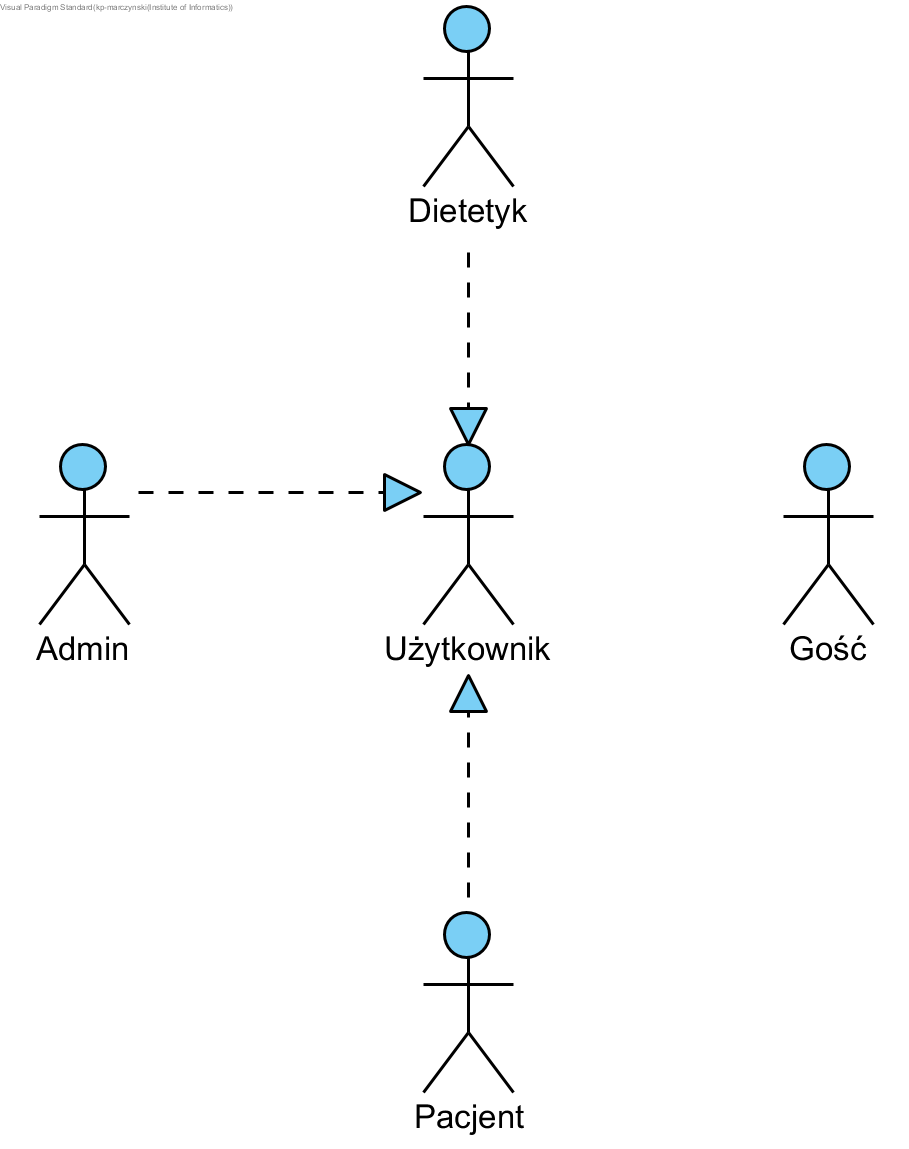
\includegraphics[scale=0.55]{../uml/use_case_diagrams/users.png}
        \caption{Użytkownicy - diagram przypadków użycia (opr.wł).}\label{rysunek:use-case-diagram-users}
    \end{figure}
\end{minipage}

\begin{minipage}{\textwidth}
    \begin{figure}[H]
        \centering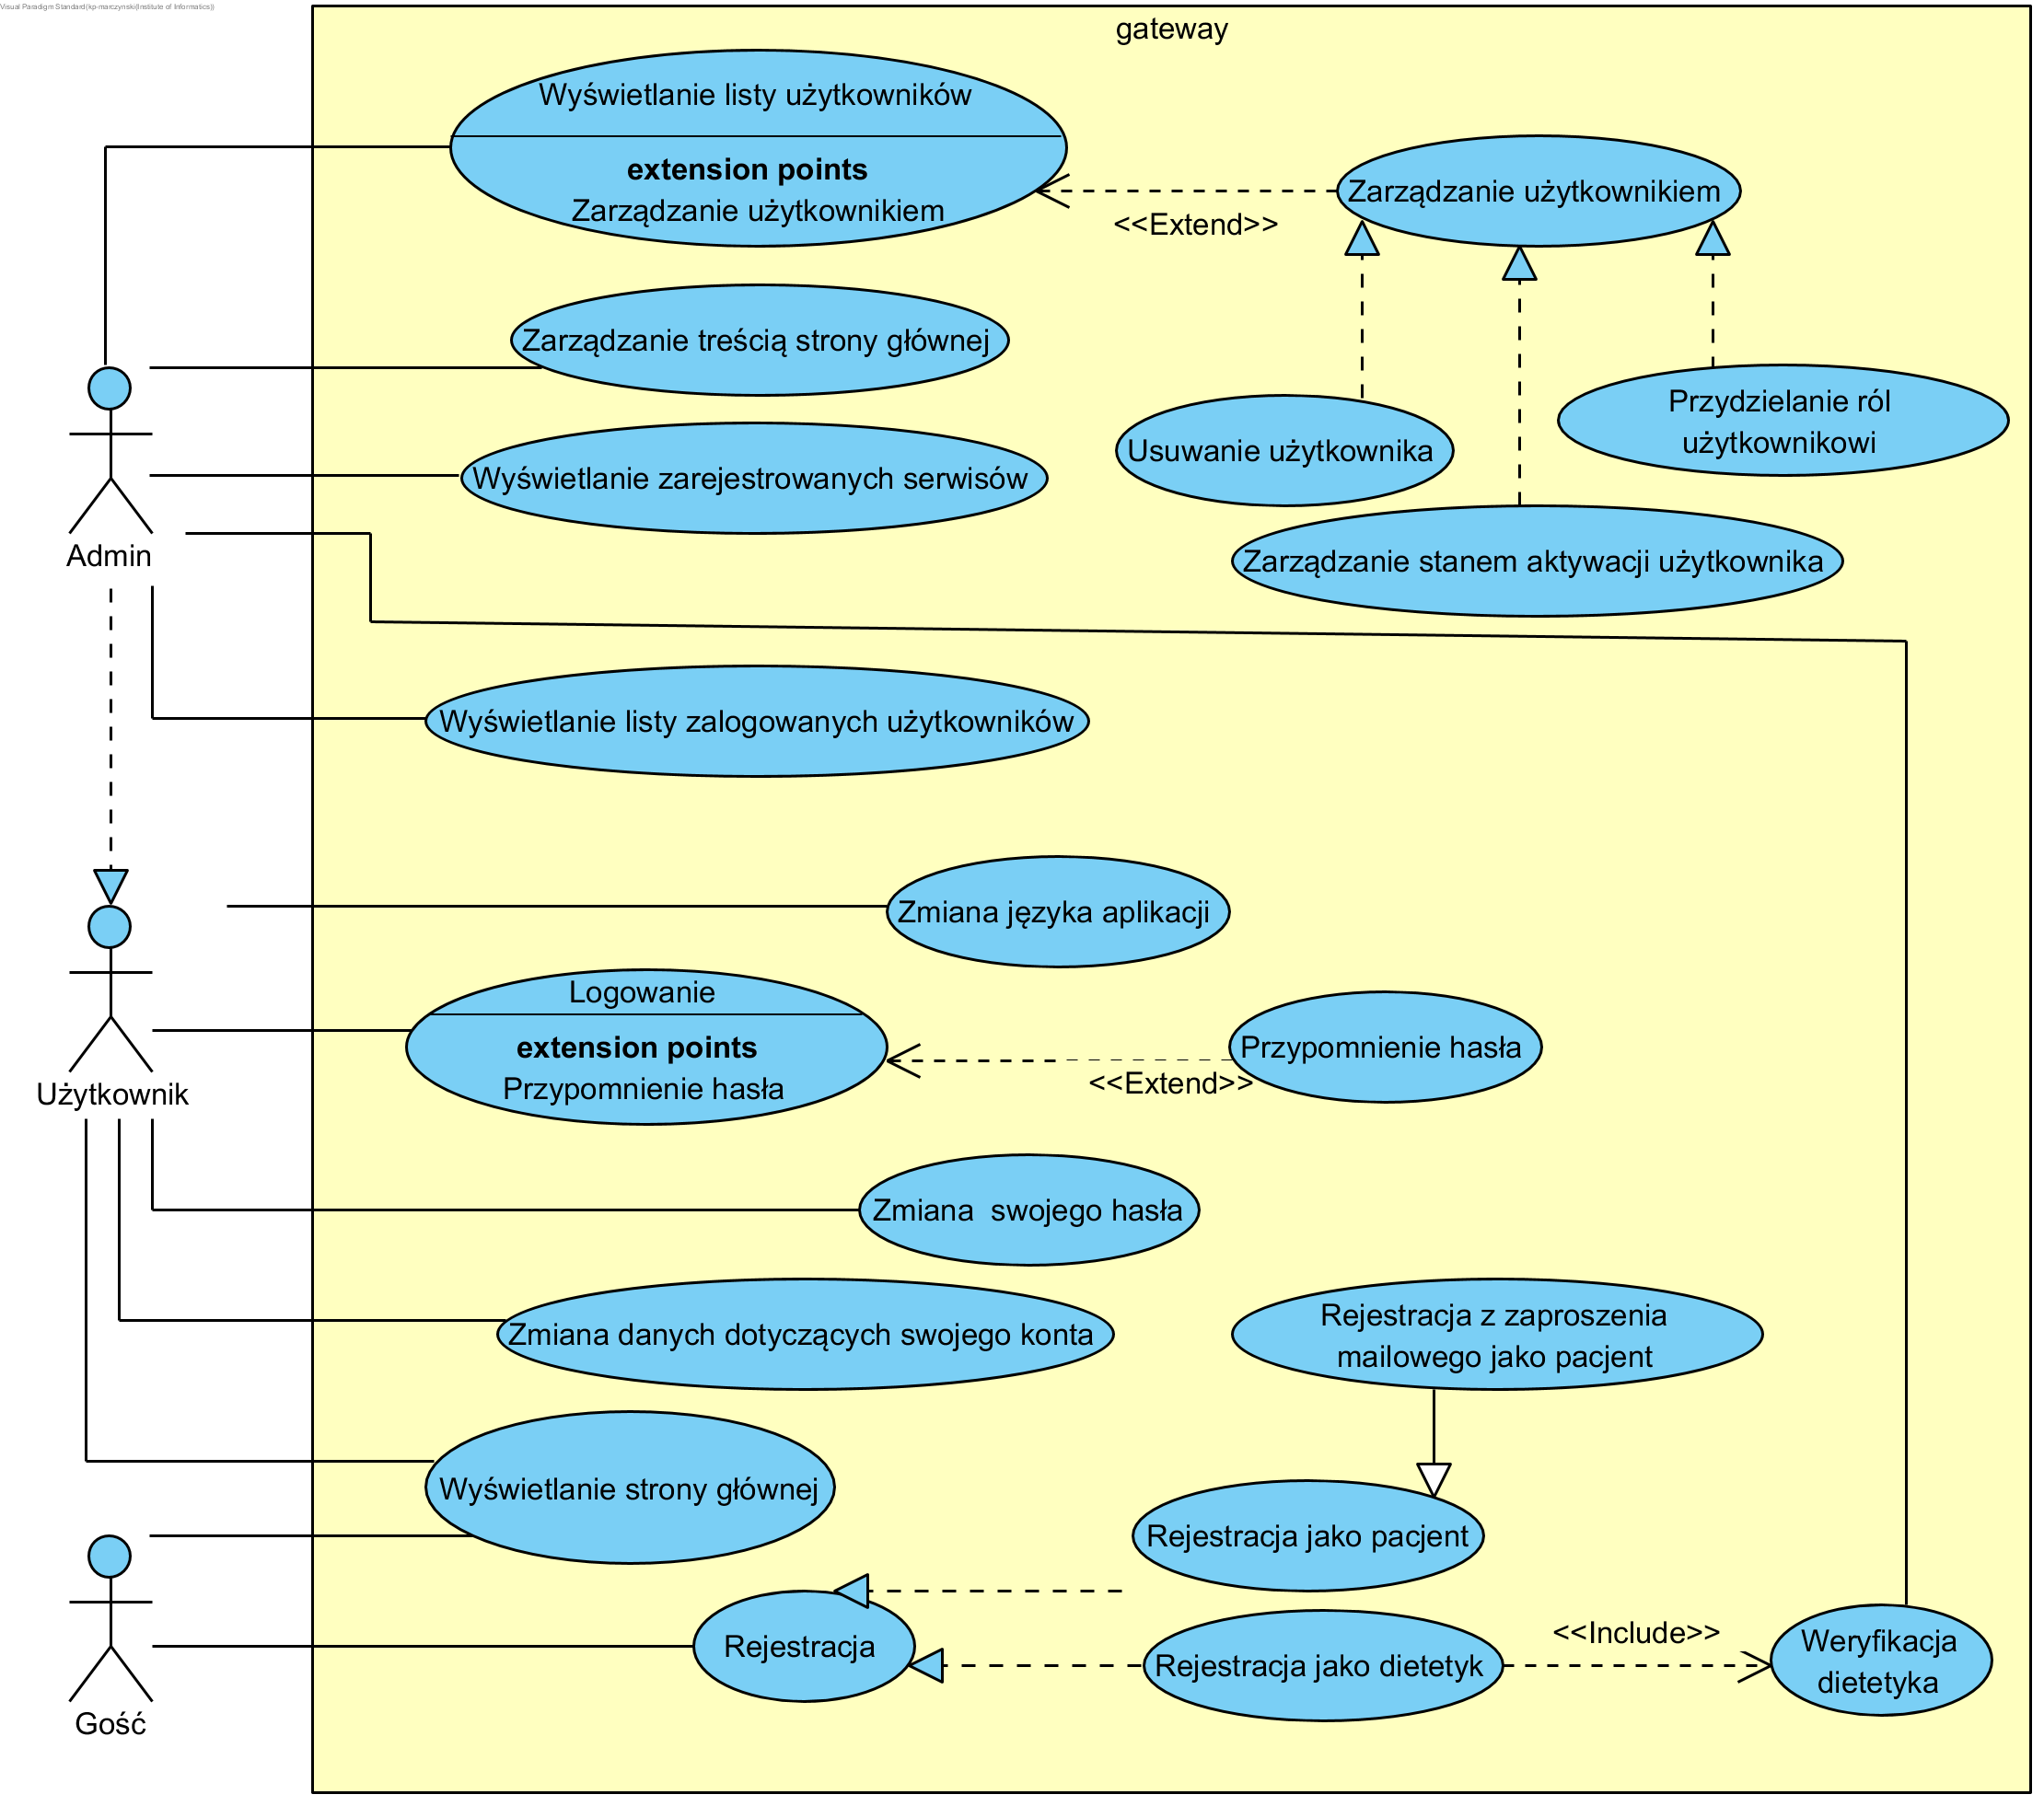
\includegraphics[scale=0.55]{../uml/use_case_diagrams/gateway.png}
        \caption{Gateway - diagram przypadków użycia (opr.wł).}\label{rysunek:use-case-diagram-gateway}
    \end{figure}
\end{minipage}

\begin{minipage}{\textwidth}
    \begin{figure}[H]
        \centering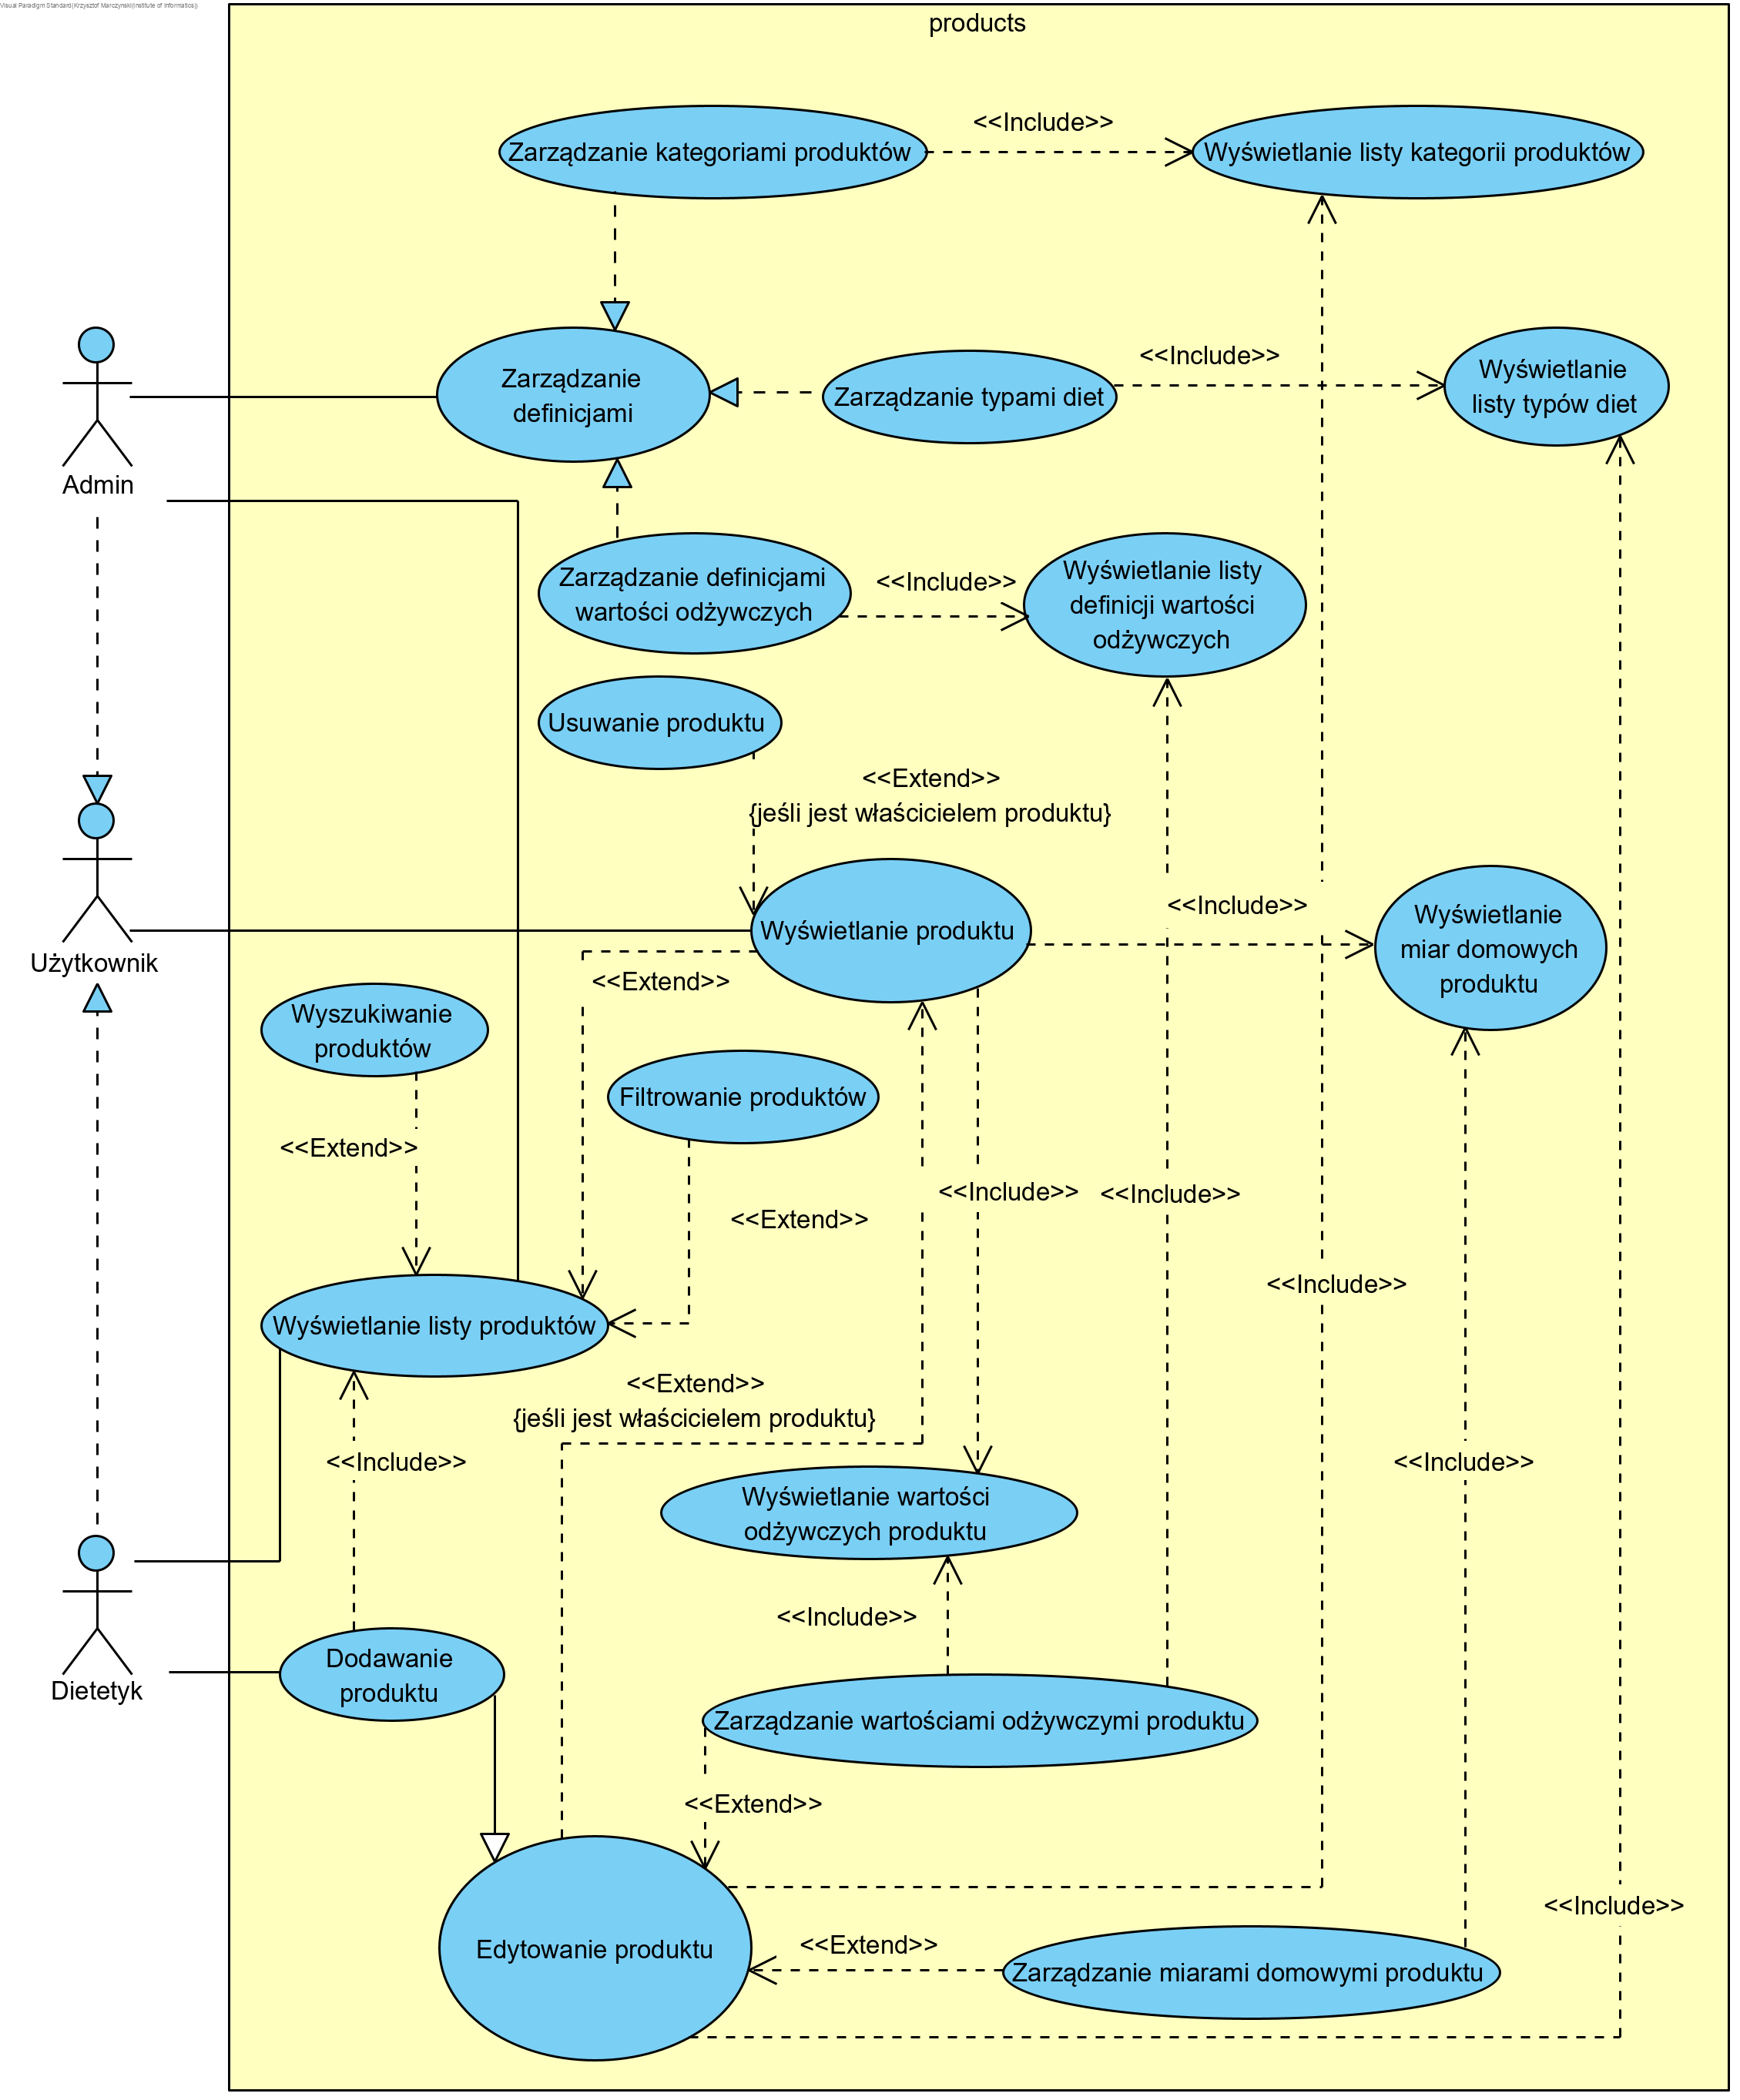
\includegraphics[scale=0.55]{../uml/use_case_diagrams/products.png}
        \caption{Produkty - diagram przypadków użycia (opr.wł).}\label{rysunek:use-case-diagram-products}
    \end{figure}
\end{minipage}

\begin{minipage}{\textwidth}
    \begin{figure}[H]
        \centering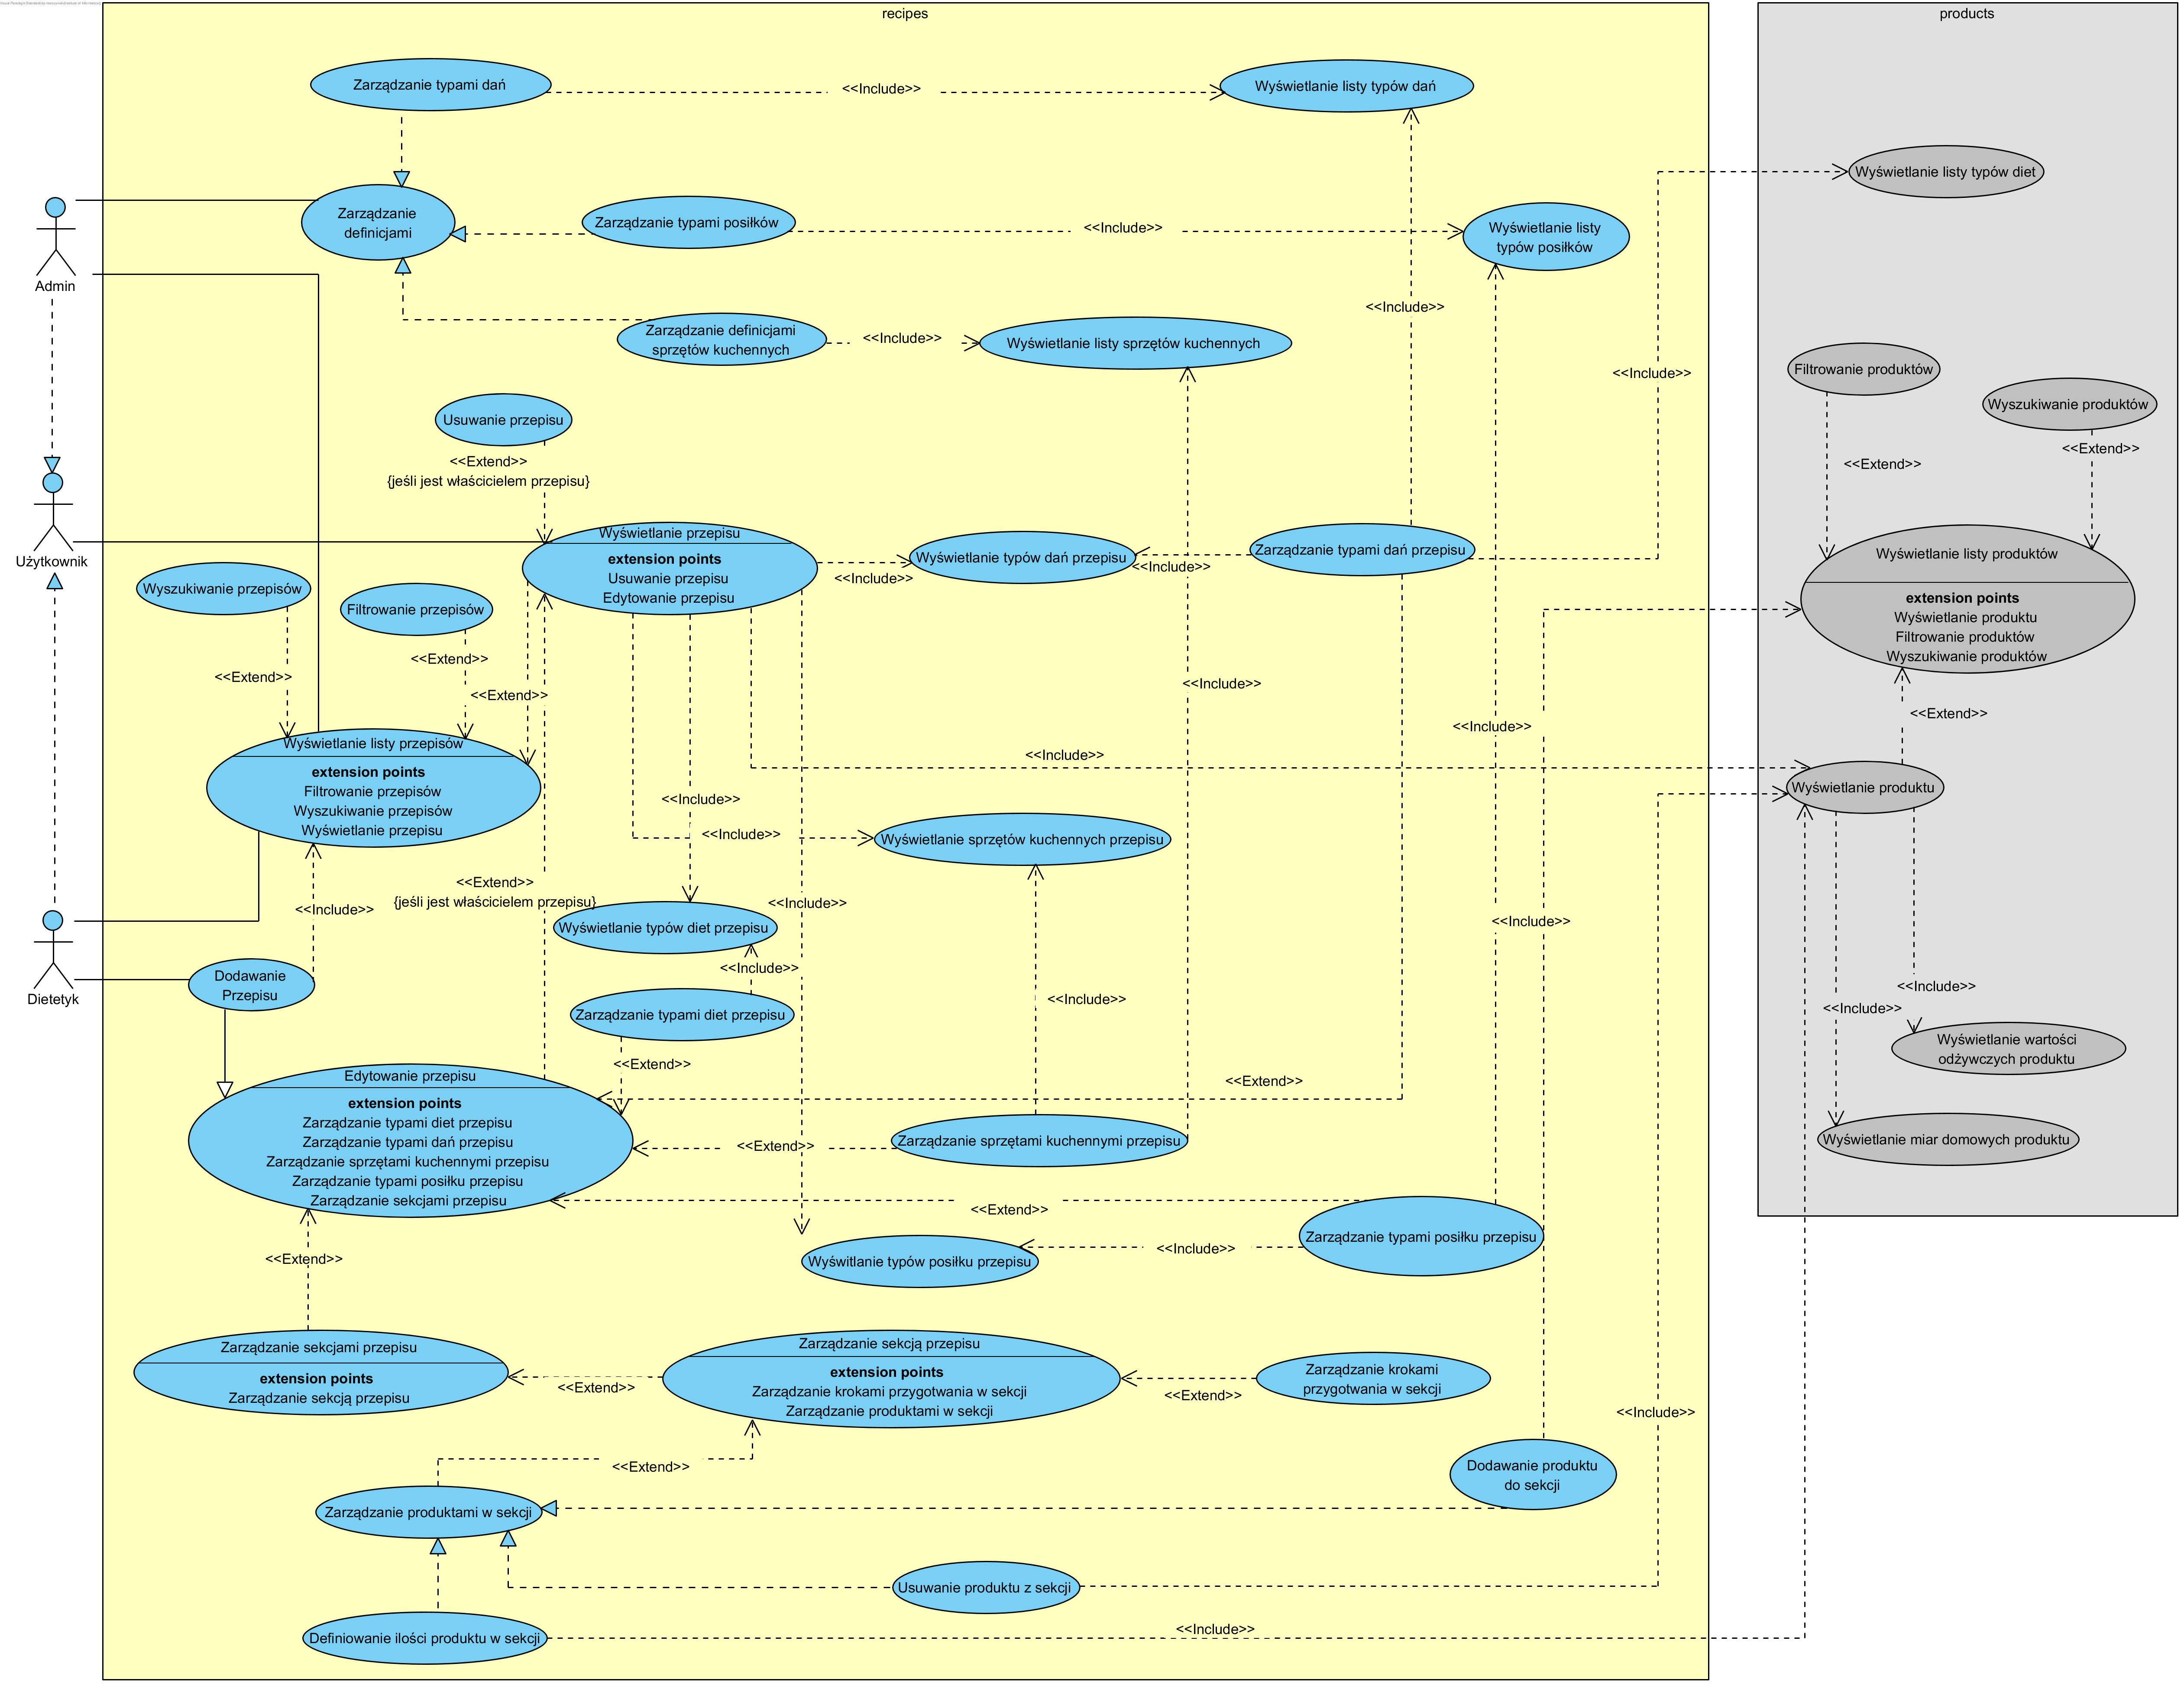
\includegraphics[scale=0.55]{../uml/use_case_diagrams/recipes.png}
        \caption{Przepisy - diagram przypadków użycia (opr.wł).}\label{rysunek:use-case-diagram-recipes}
    \end{figure}
\end{minipage}

\begin{minipage}{\textwidth}
    \begin{figure}[H]
        \centering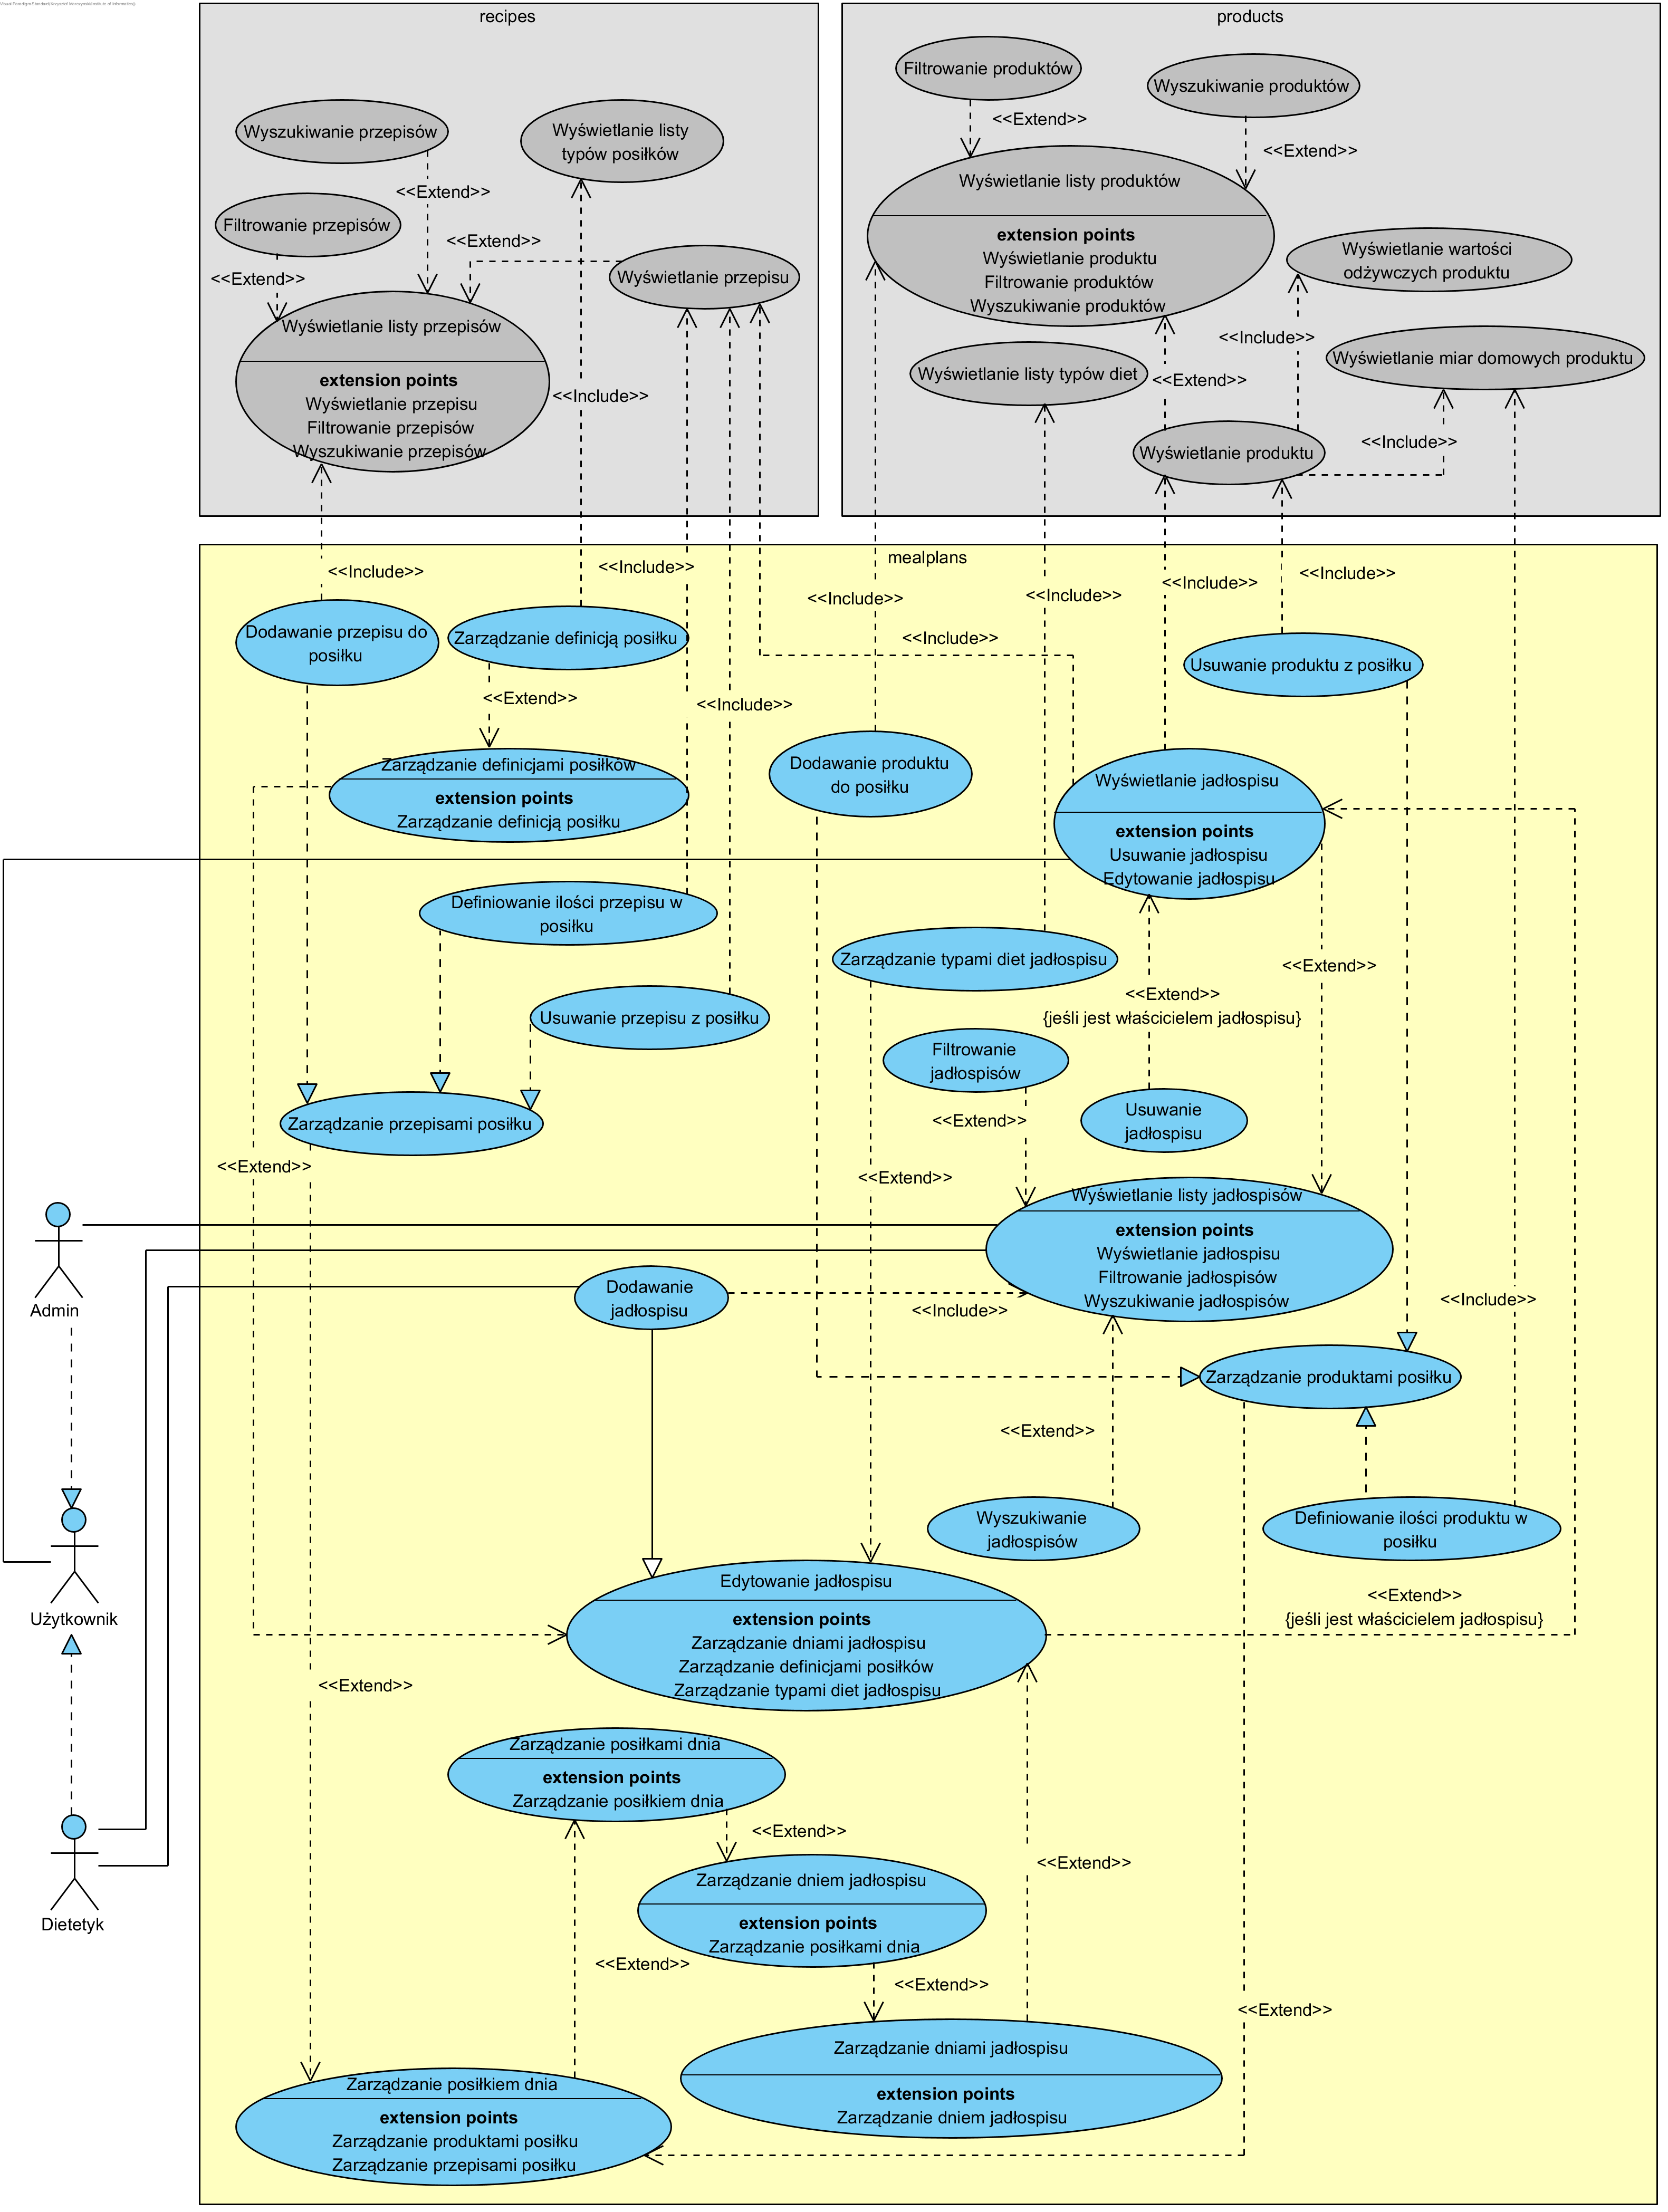
\includegraphics[scale=0.55]{../uml/use_case_diagrams/mealplans.png}
        \caption{Jadłospisy - diagram przypadków użycia (opr.wł).}\label{rysunek:use-case-diagram-mealplans}
    \end{figure}
\end{minipage}

\begin{minipage}{\textwidth}
    \begin{figure}[H]
        \centering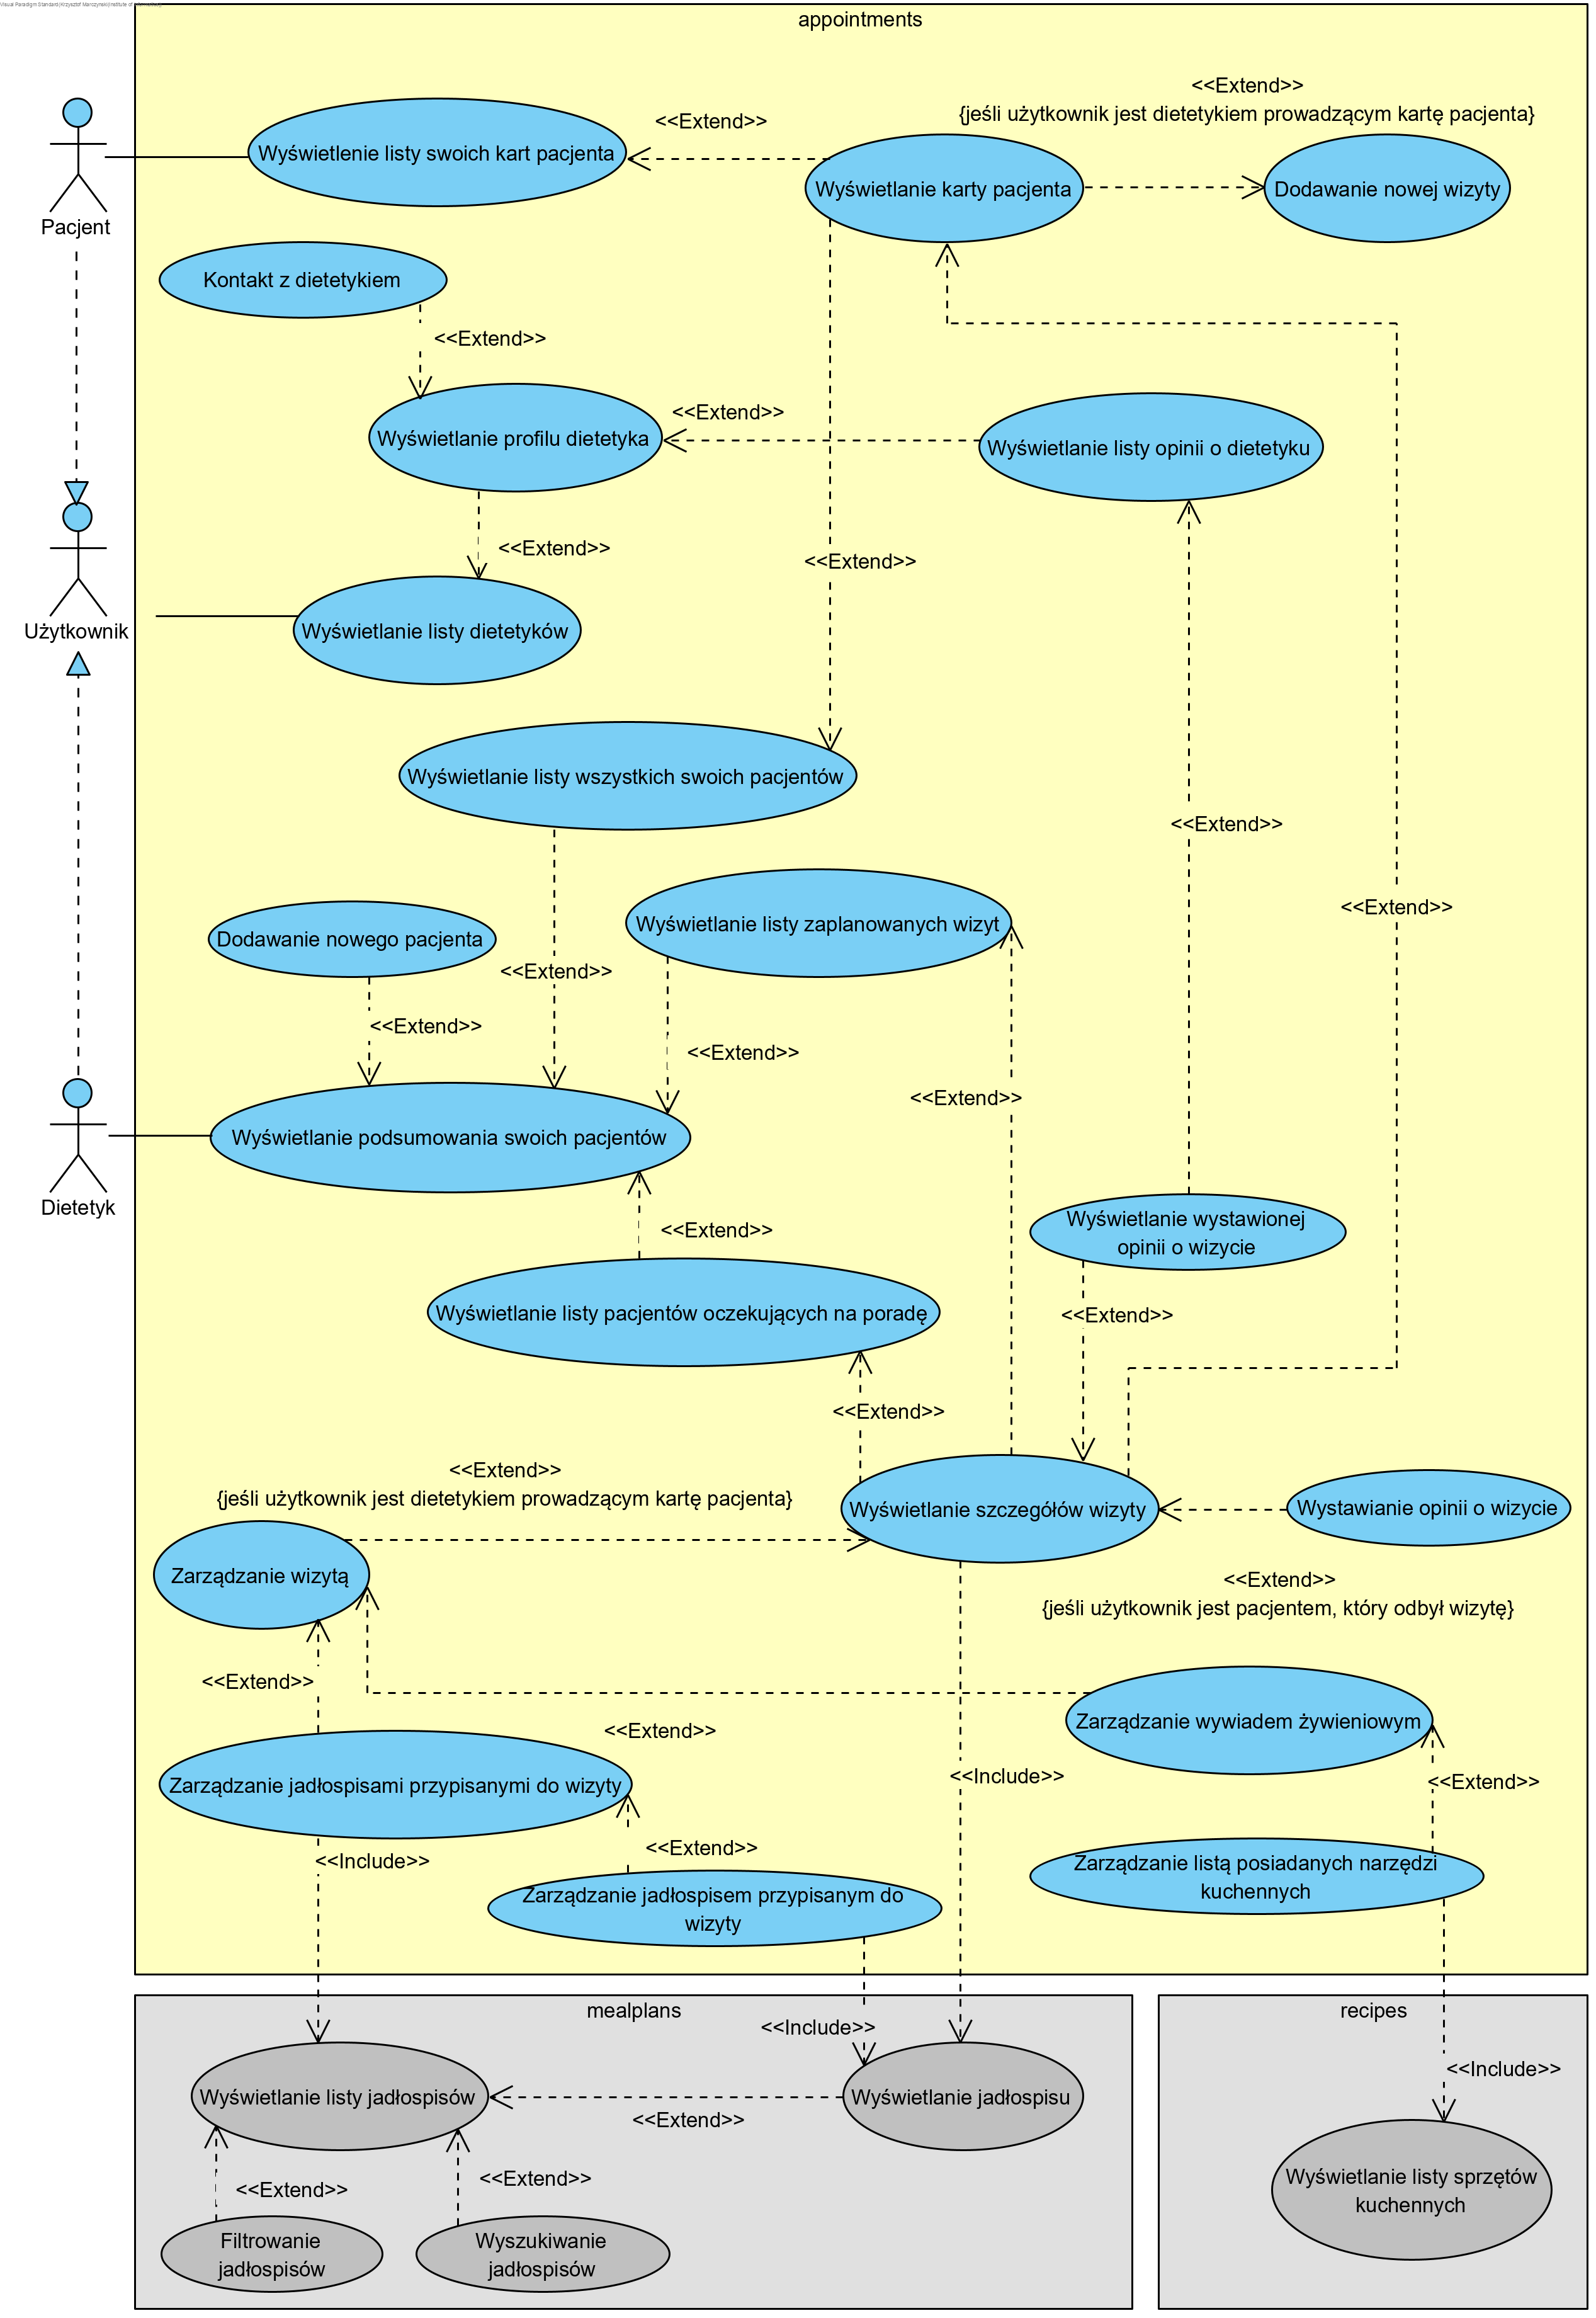
\includegraphics[scale=0.55]{../uml/use_case_diagrams/appointments.png}
        \caption{Wizyty - diagram przypadków użycia (opr.wł).}\label{rysunek:use-case-diagram-appointments}
    \end{figure}
\end{minipage}

\section{Prototyp interfejsu}
\todo{mockupy}
\begin{minipage}{\textwidth}
    \begin{figure}[H]
        \centering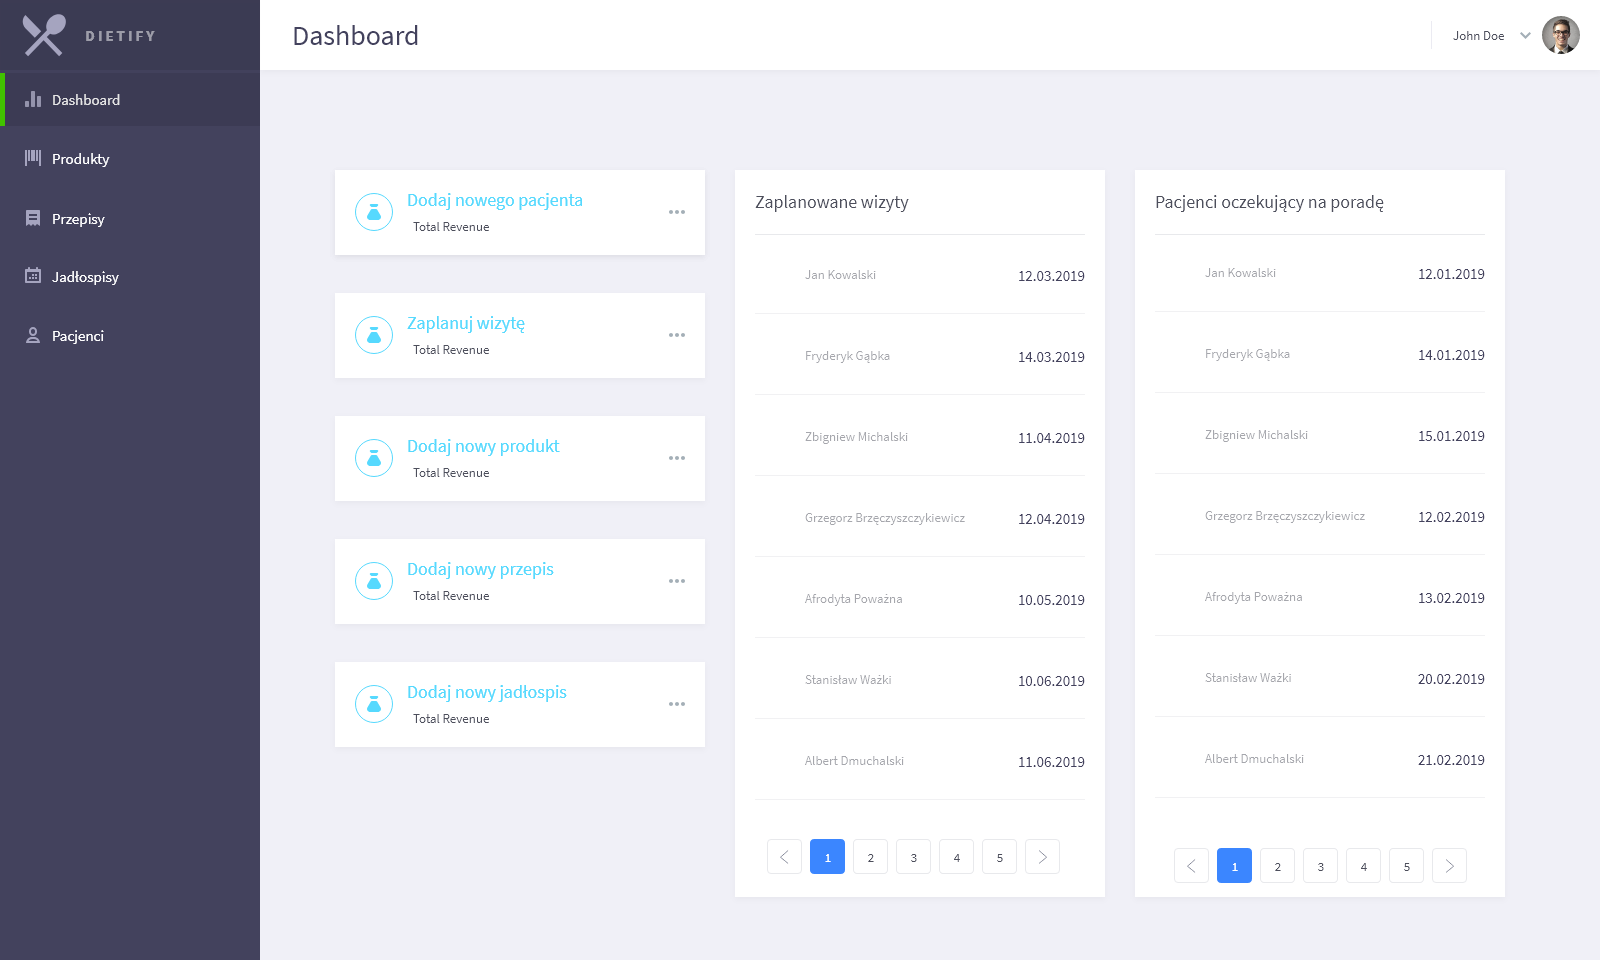
\includegraphics[width=0.9\textwidth]{img/mockups/mockup1.png}
        \caption{Mockup1 (opr.wł).}\label{rysunek:mockup1}
    \end{figure}
\end{minipage}

\begin{minipage}{\textwidth}
    \begin{figure}[H]
        \centering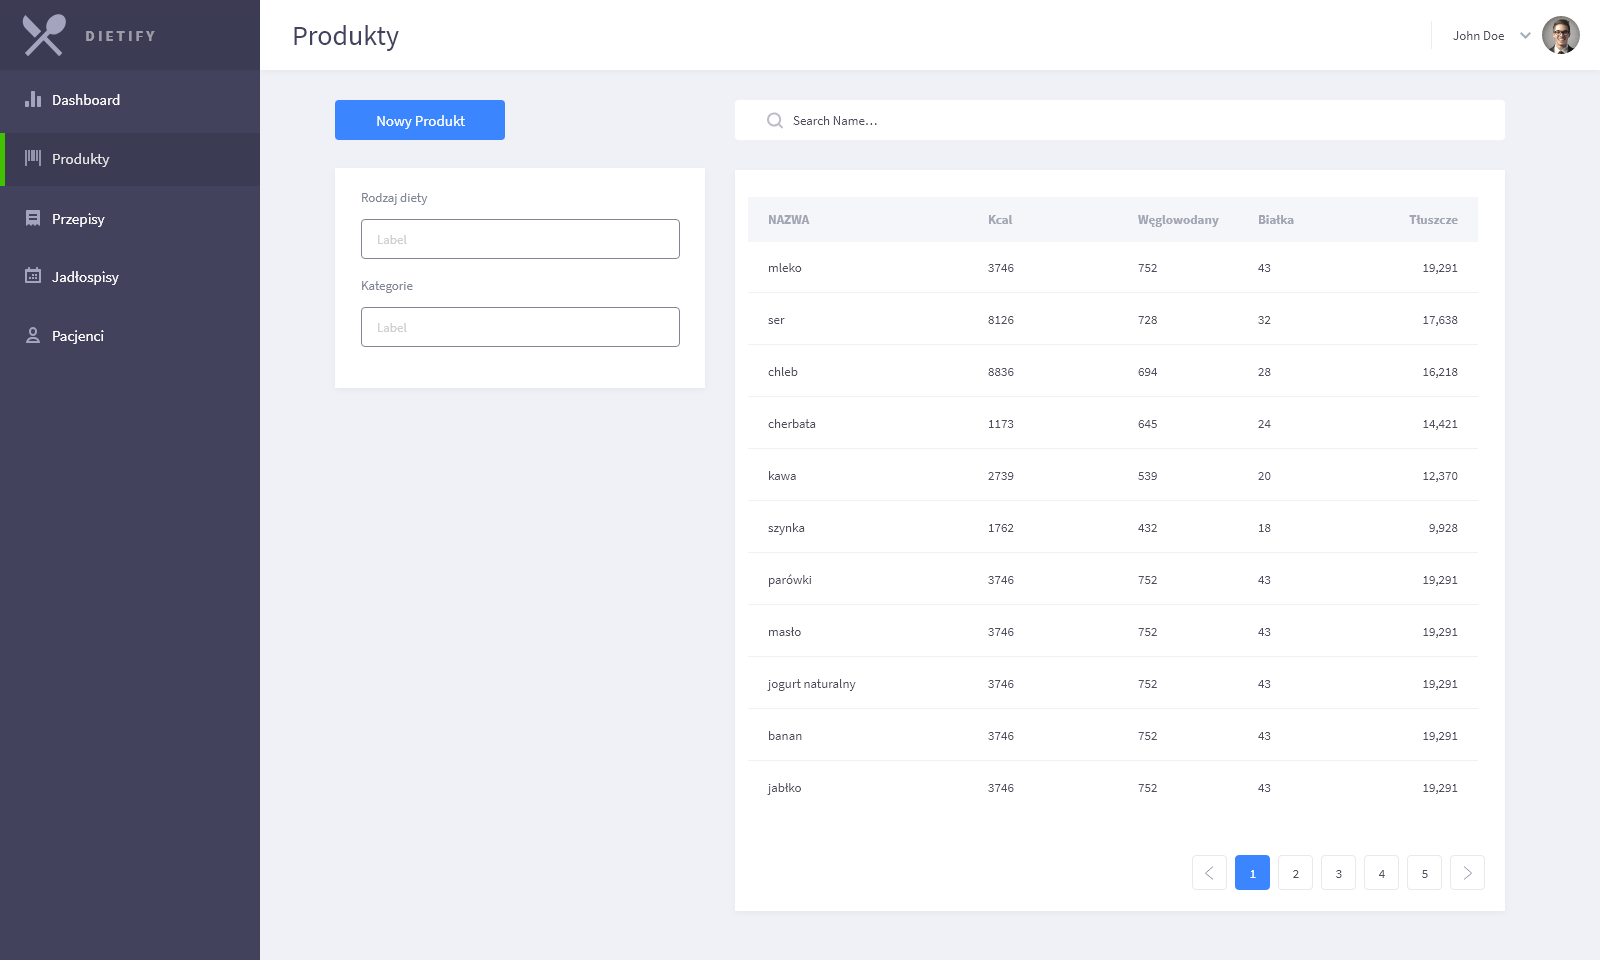
\includegraphics[width=0.9\textwidth]{img/mockups/mockup2.png}
        \caption{Mockup2 (opr.wł).}\label{rysunek:mockup2}
    \end{figure}
\end{minipage}

\begin{minipage}{\textwidth}
    \begin{figure}[H]
        \centering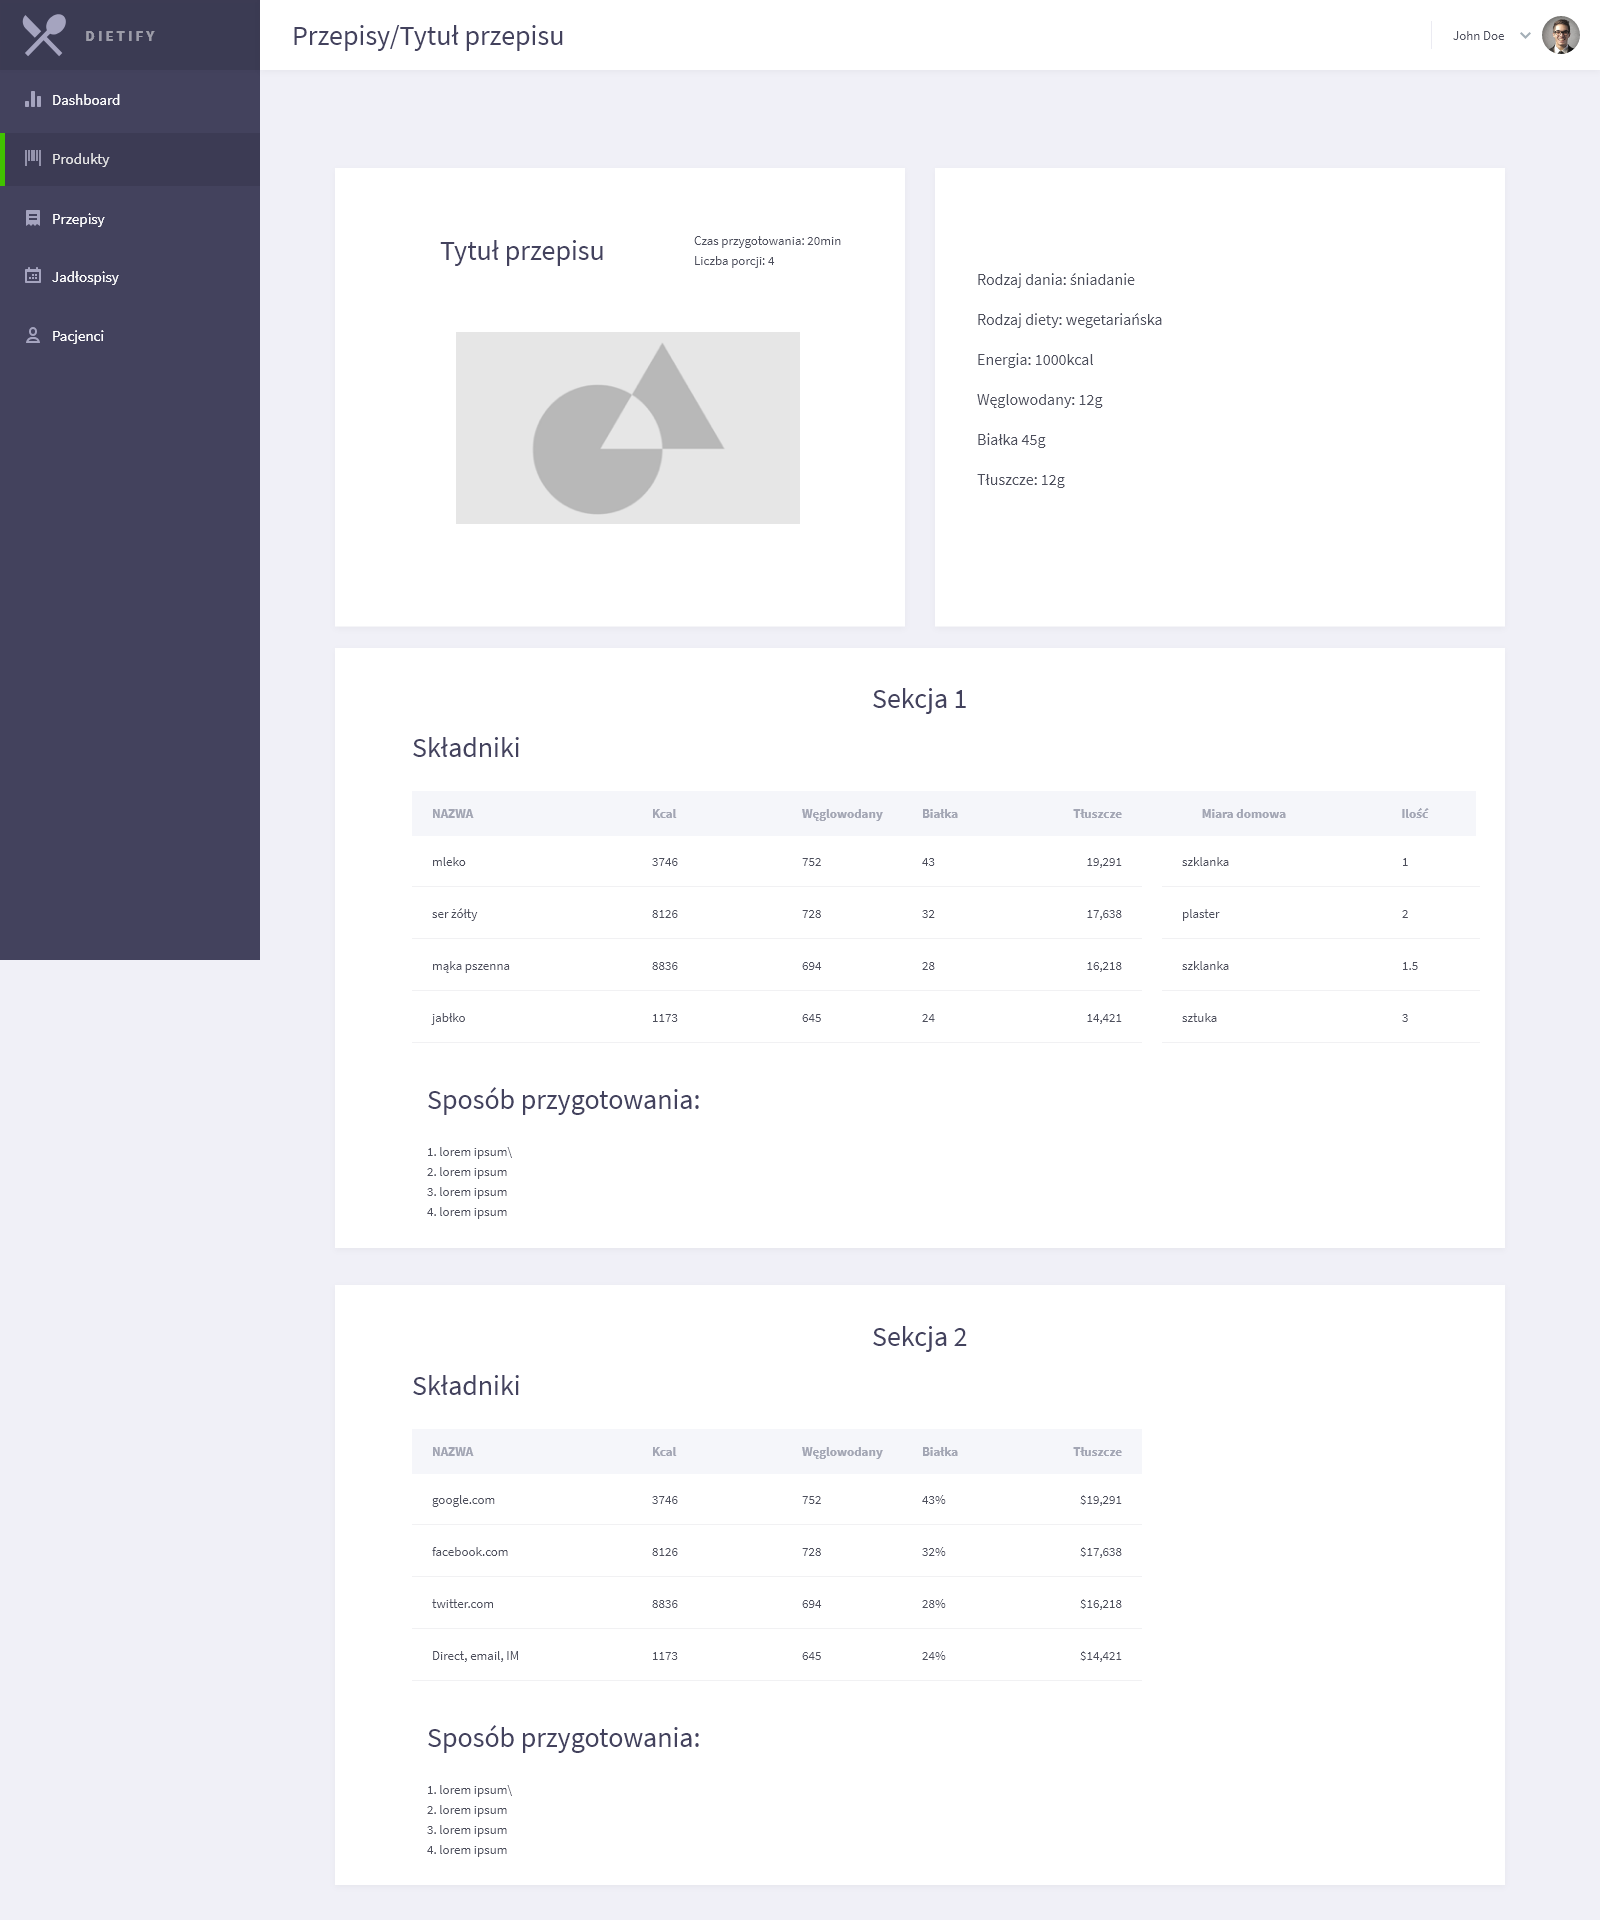
\includegraphics[width=0.9\textwidth]{img/mockups/mockup3.png}
        \caption{Mockup3 (opr.wł).}\label{rysunek:mockup3}
    \end{figure}
\end{minipage}

\begin{minipage}{\textwidth}
    \begin{figure}[H]
        \centering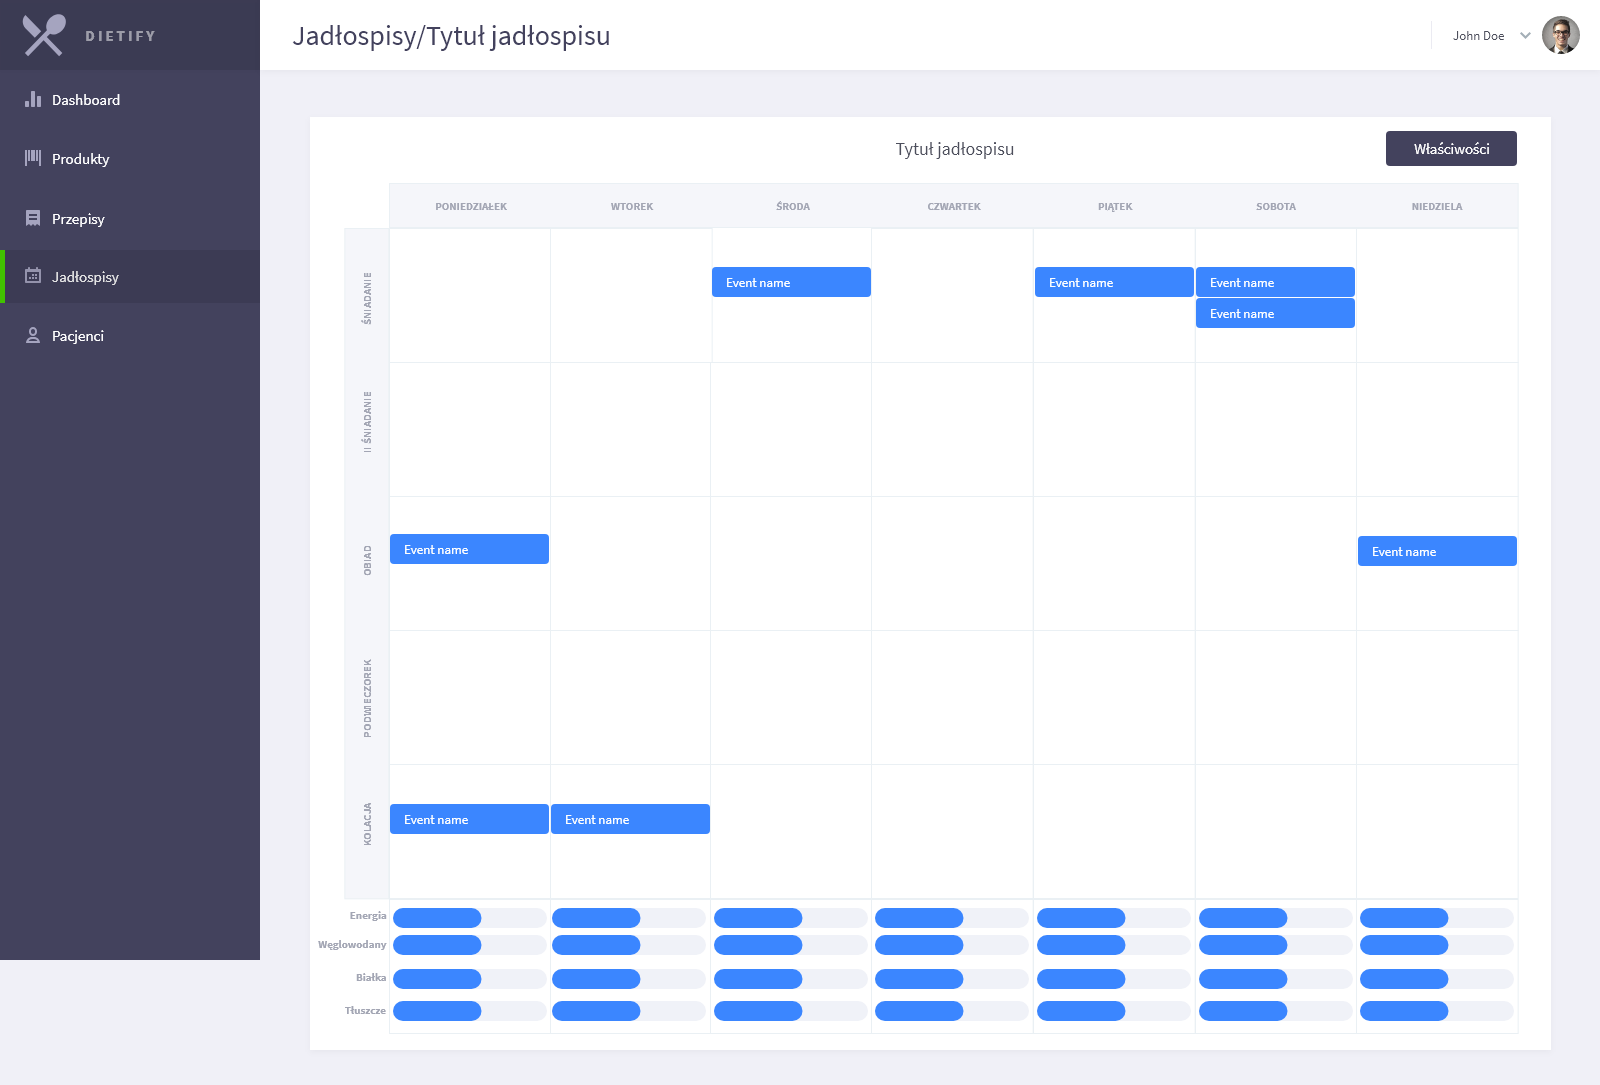
\includegraphics[width=0.9\textwidth]{img/mockups/mockup4.png}
        \caption{Mockup4 (opr.wł).}\label{rysunek:mockup4}
    \end{figure}
\end{minipage}

\begin{minipage}{\textwidth}
    \begin{figure}[H]
        \centering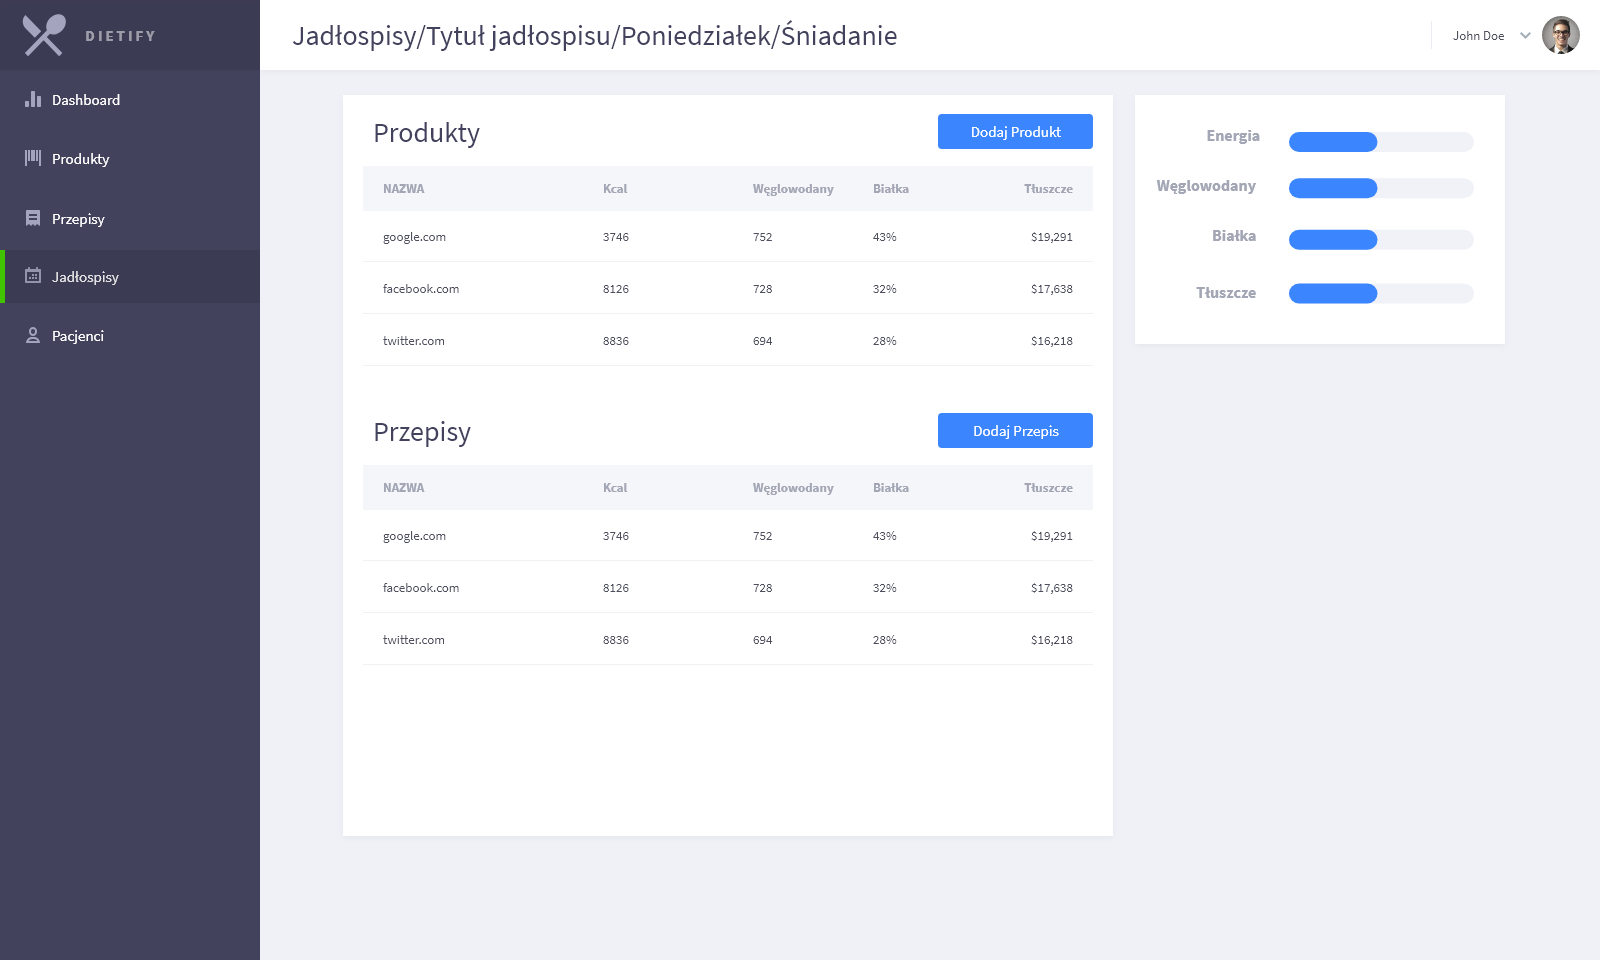
\includegraphics[width=0.9\textwidth]{img/mockups/mockup5.png}
        \caption{Mockup5 (opr.wł).}\label{rysunek:mockup5}
    \end{figure}
\end{minipage}

\begin{minipage}{\textwidth}
    \begin{figure}[H]
        \centering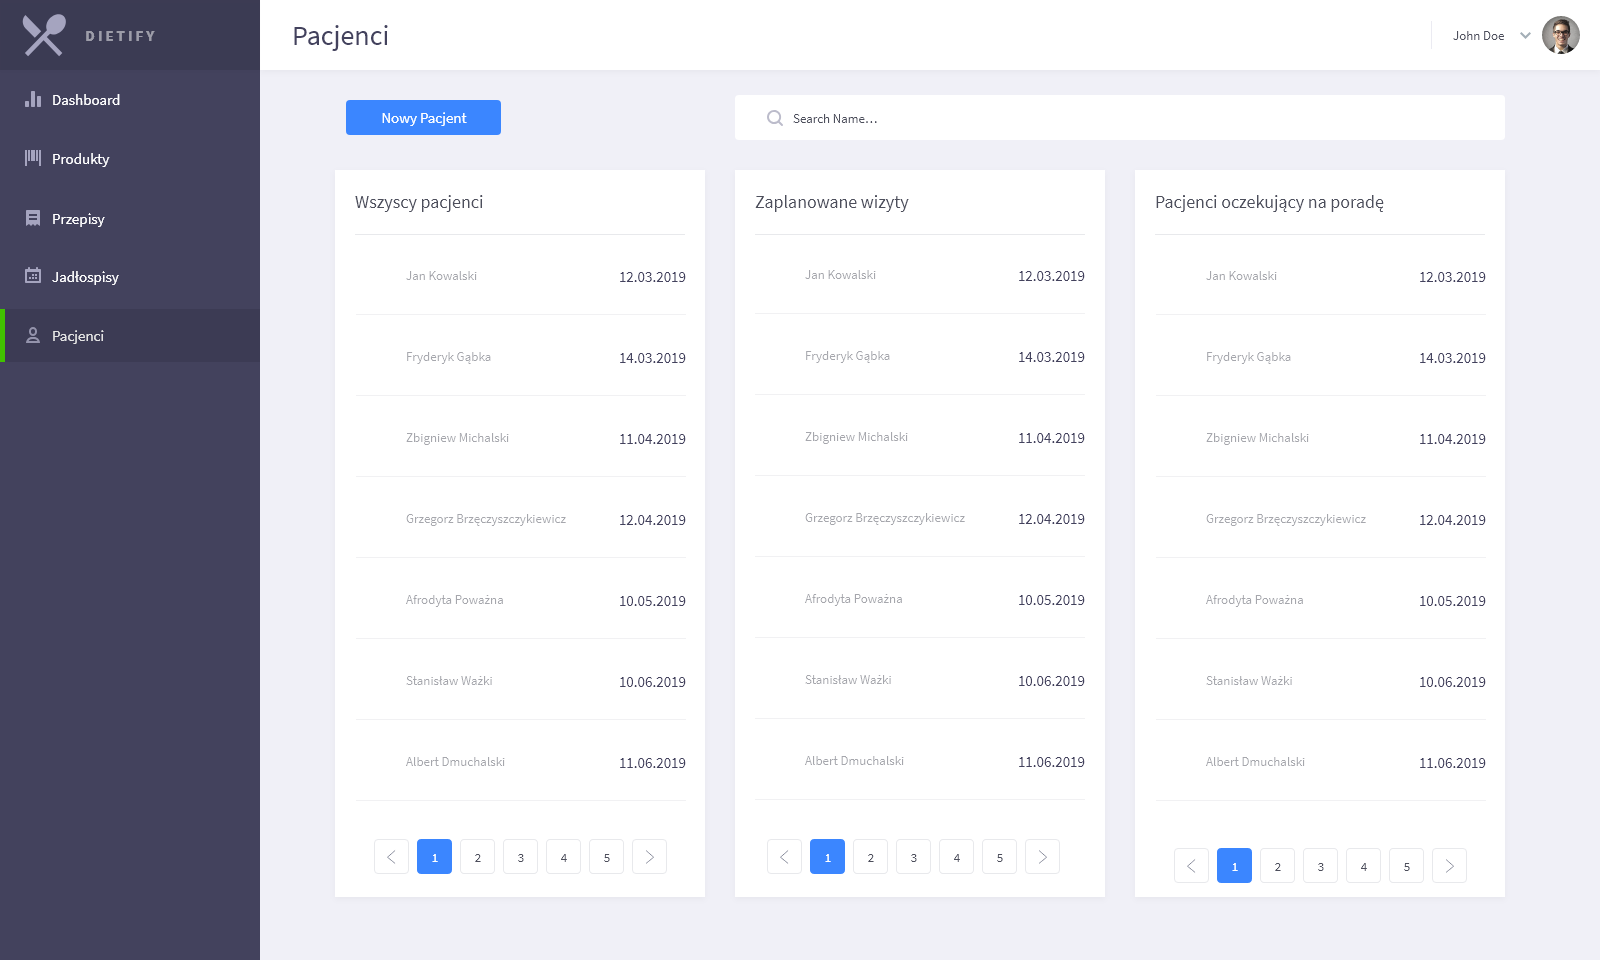
\includegraphics[width=0.9\textwidth]{img/mockups/mockup6.png}
        \caption{Mockup6 (opr.wł).}\label{rysunek:mockup6}
    \end{figure}
\end{minipage}

\begin{minipage}{\textwidth}
    \begin{figure}[H]
        \centering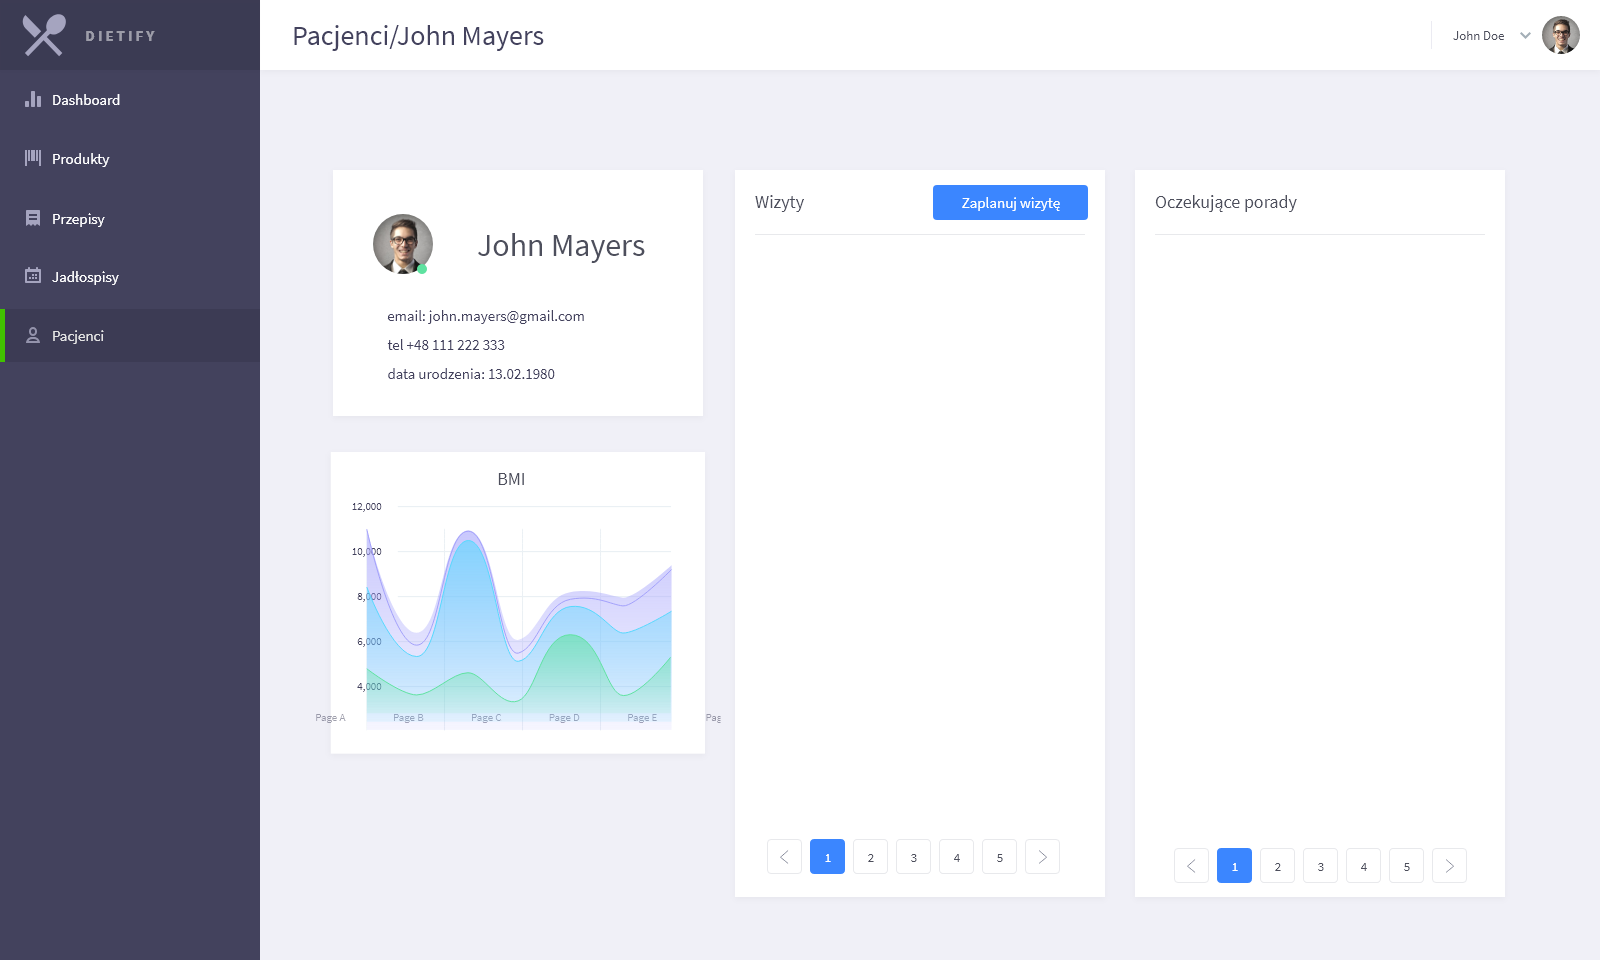
\includegraphics[width=0.9\textwidth]{img/mockups/mockup7.png}
        \caption{Mockup7 (opr.wł).}\label{rysunek:mockup7}
    \end{figure}
\end{minipage}

\begin{minipage}{\textwidth}
    \begin{figure}[H]
        \centering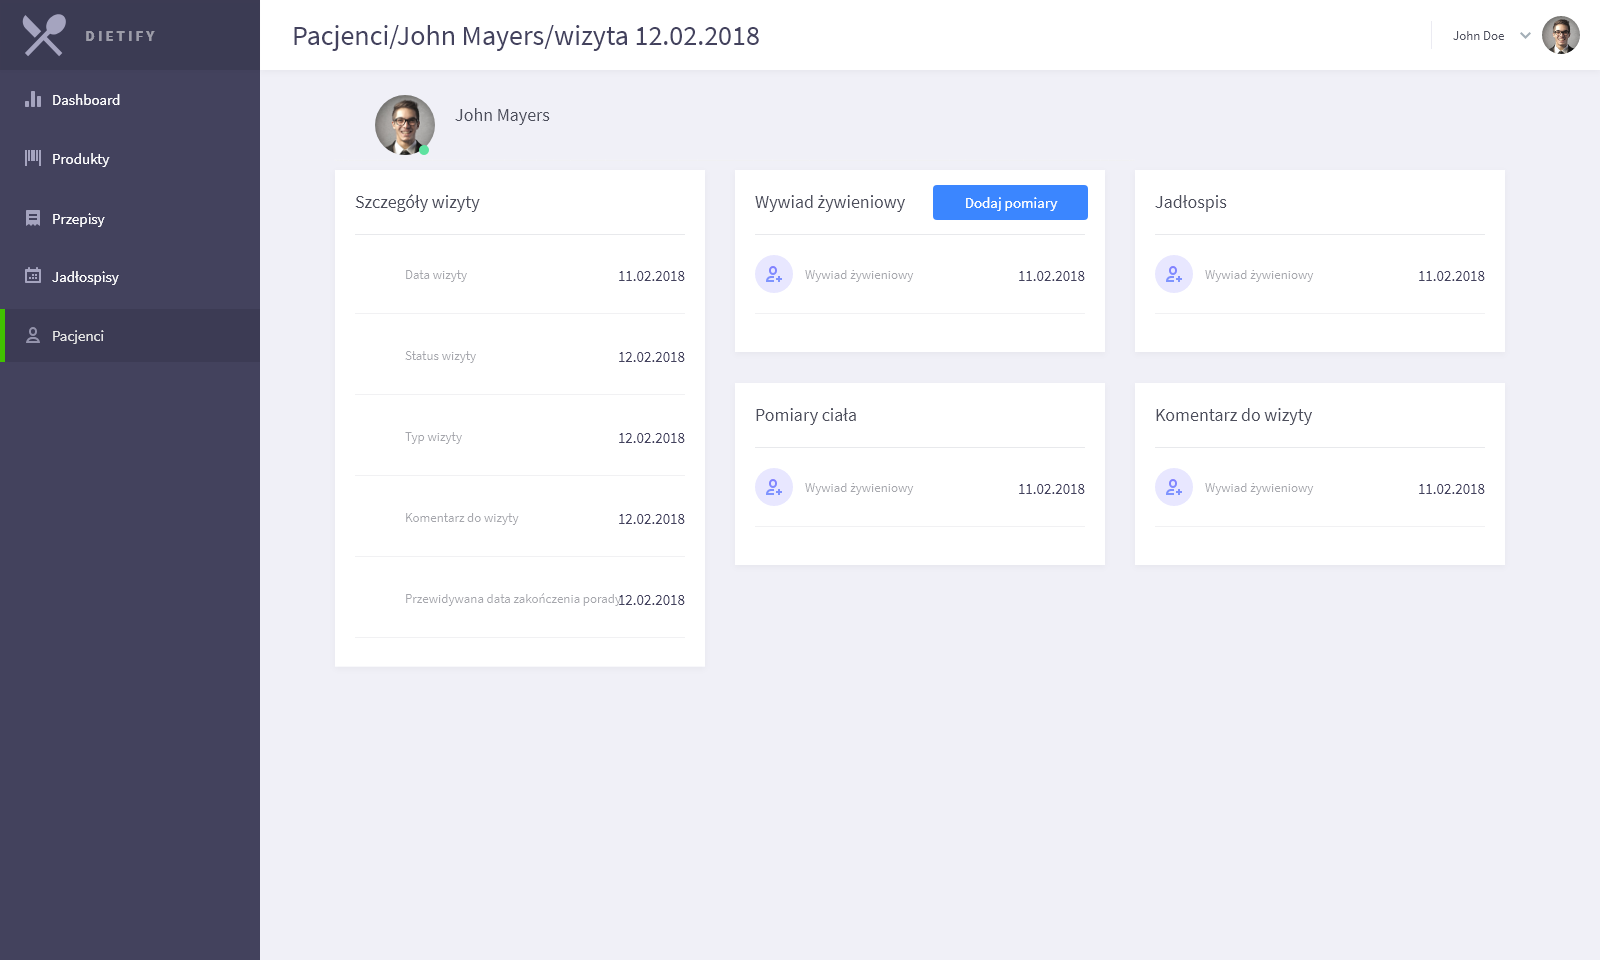
\includegraphics[width=0.9\textwidth]{img/mockups/mockup8.png}
        \caption{Mockup8 (opr.wł).}\label{rysunek:mockup8}
    \end{figure}
\end{minipage}

\begin{minipage}{\textwidth}
    \begin{figure}[H]
        \centering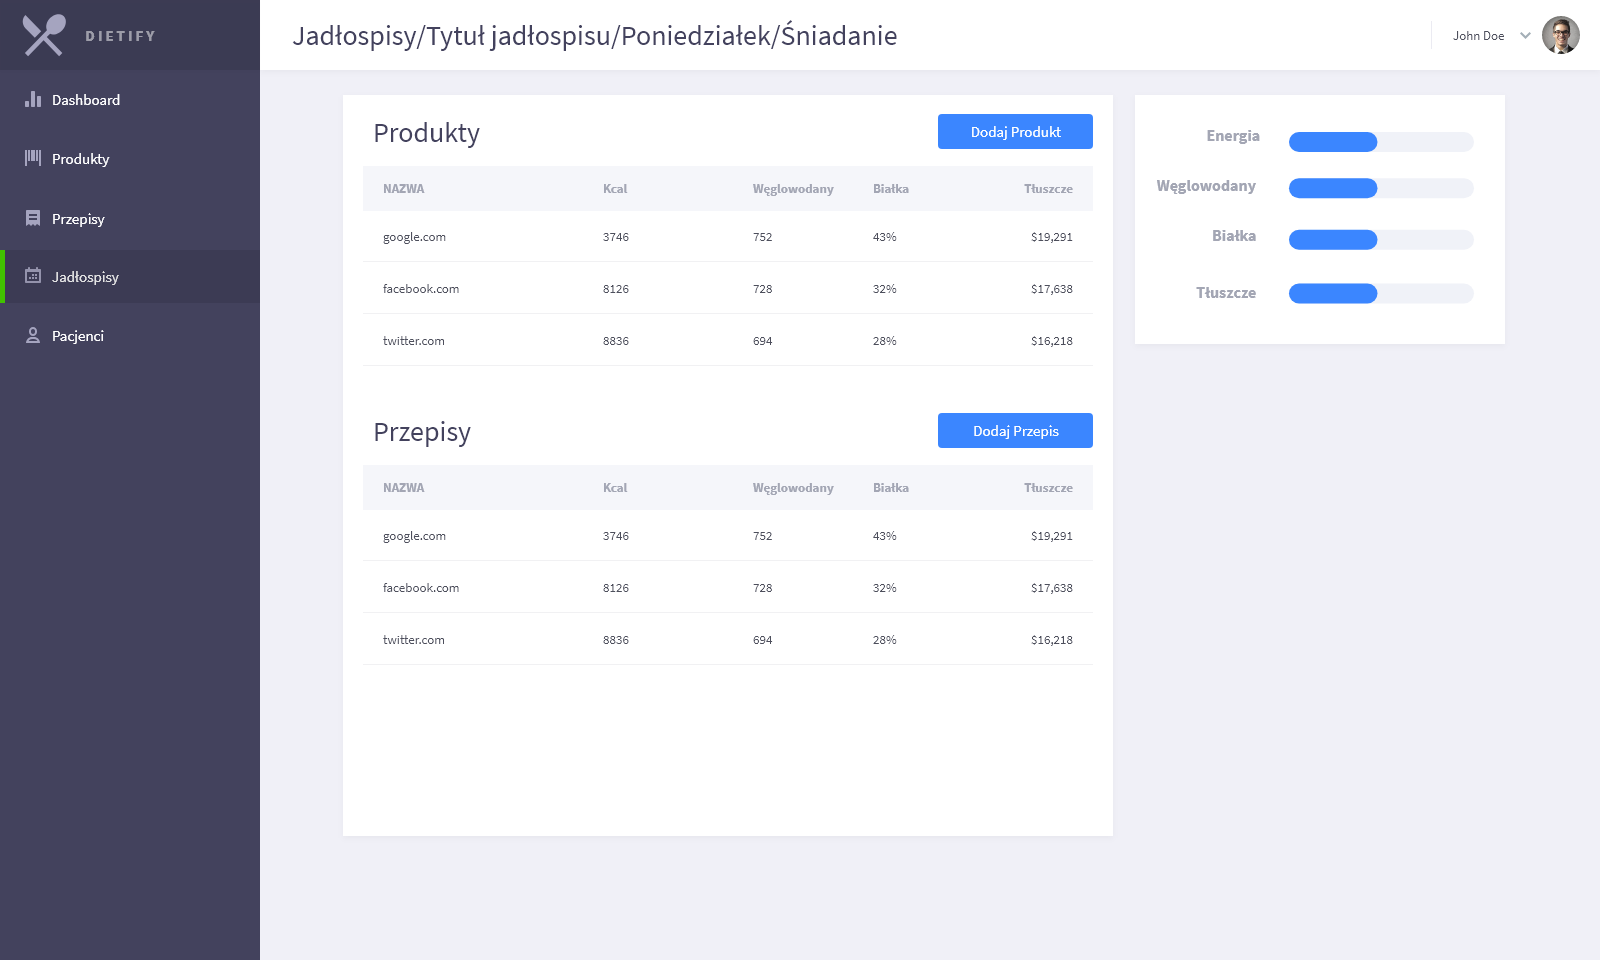
\includegraphics[width=0.9\textwidth]{img/mockups/mockup9.png}
        \caption{Mockup9 (opr.wł).}\label{rysunek:mockup9}
    \end{figure}
\end{minipage}

\begin{minipage}{\textwidth}
    \begin{figure}[H]
        \centering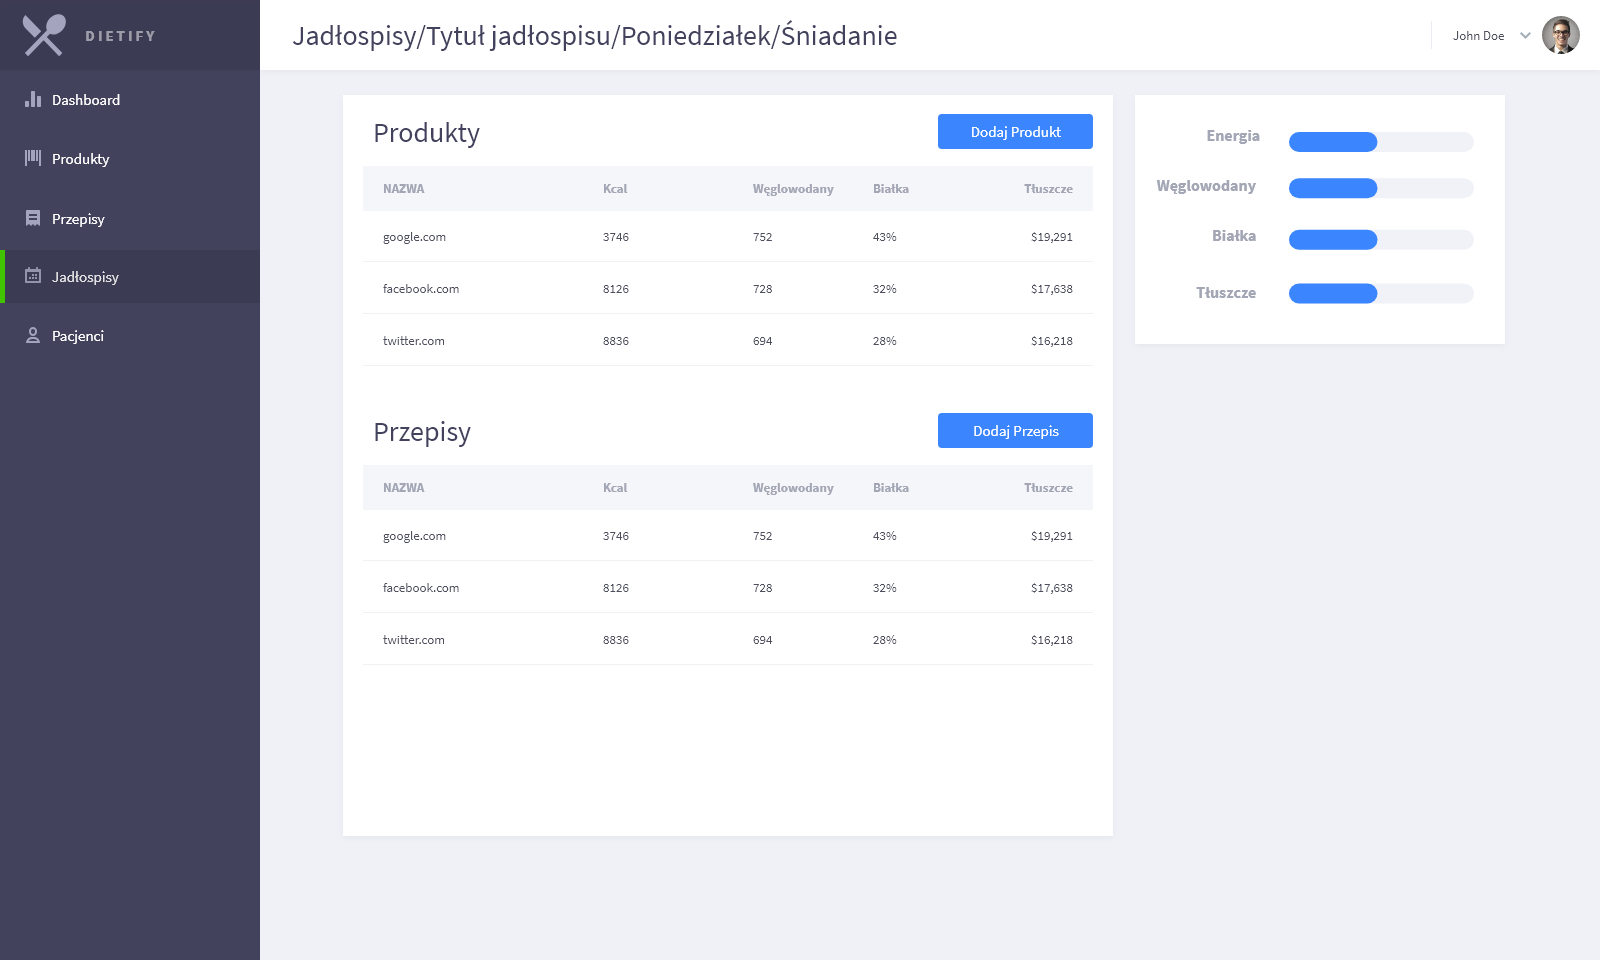
\includegraphics[width=0.9\textwidth]{img/mockups/mockup10.png}
        \caption{Mockup10 (opr.wł).}\label{rysunek:mockup10}
    \end{figure}
\end{minipage}

\begin{minipage}{\textwidth}
    \begin{figure}[H]
        \centering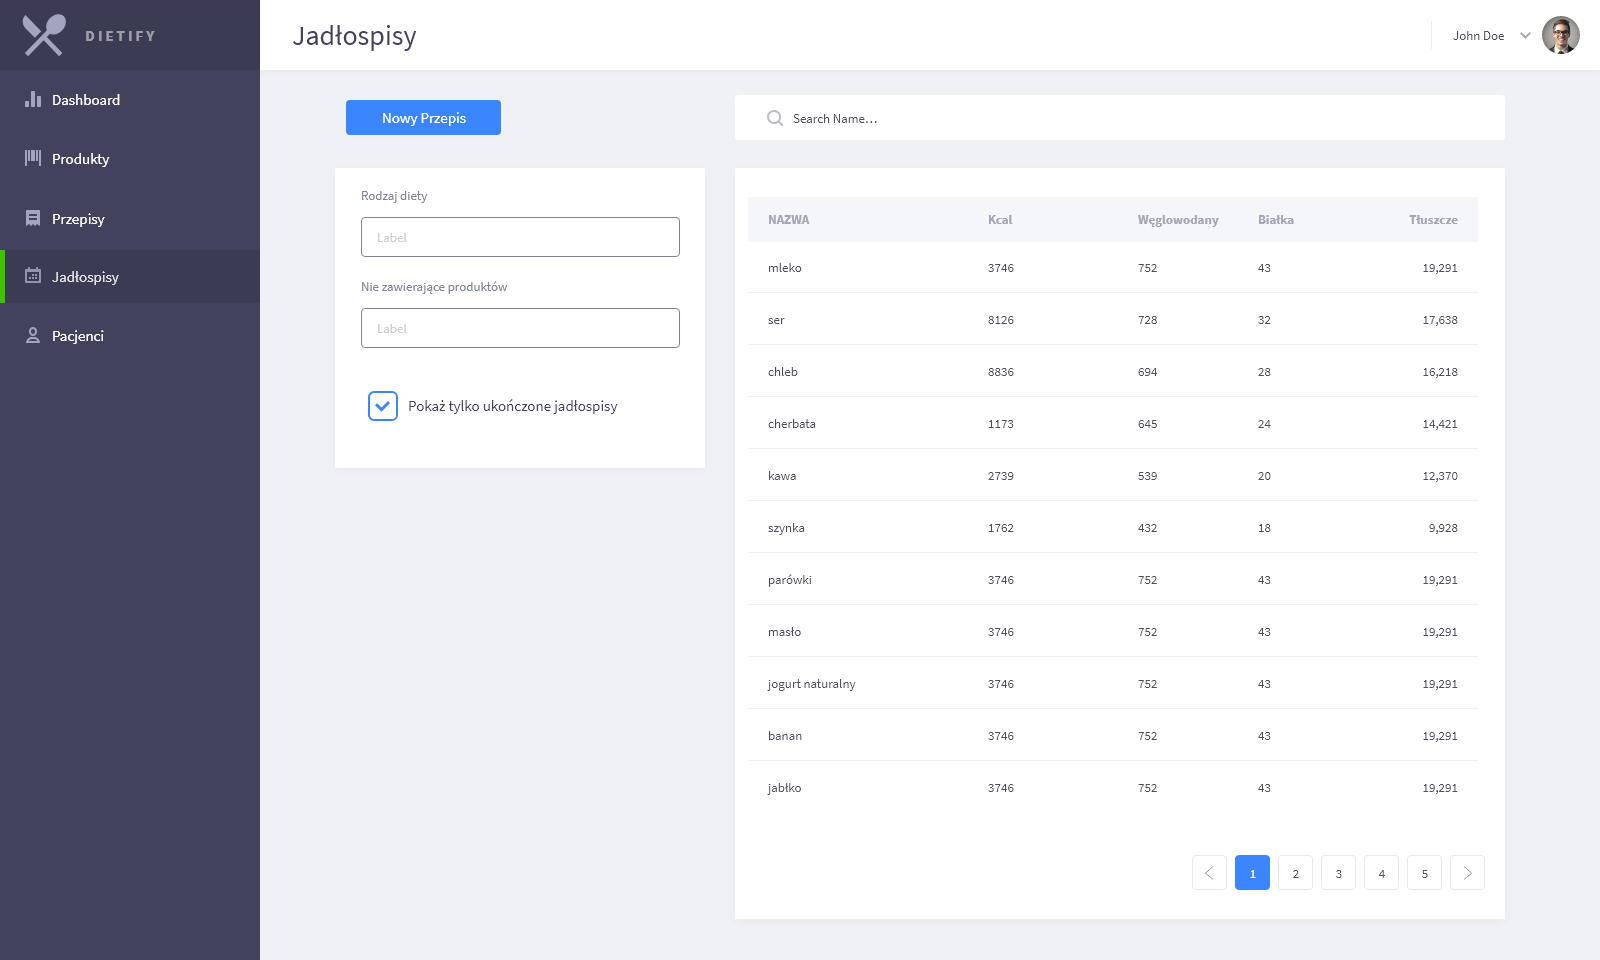
\includegraphics[width=0.9\textwidth]{img/mockups/mockup11.png}
        \caption{Mockup11 (opr.wł).}\label{rysunek:mockup11}
    \end{figure}
\end{minipage}

\begin{minipage}{\textwidth}
    \begin{figure}[H]
        \centering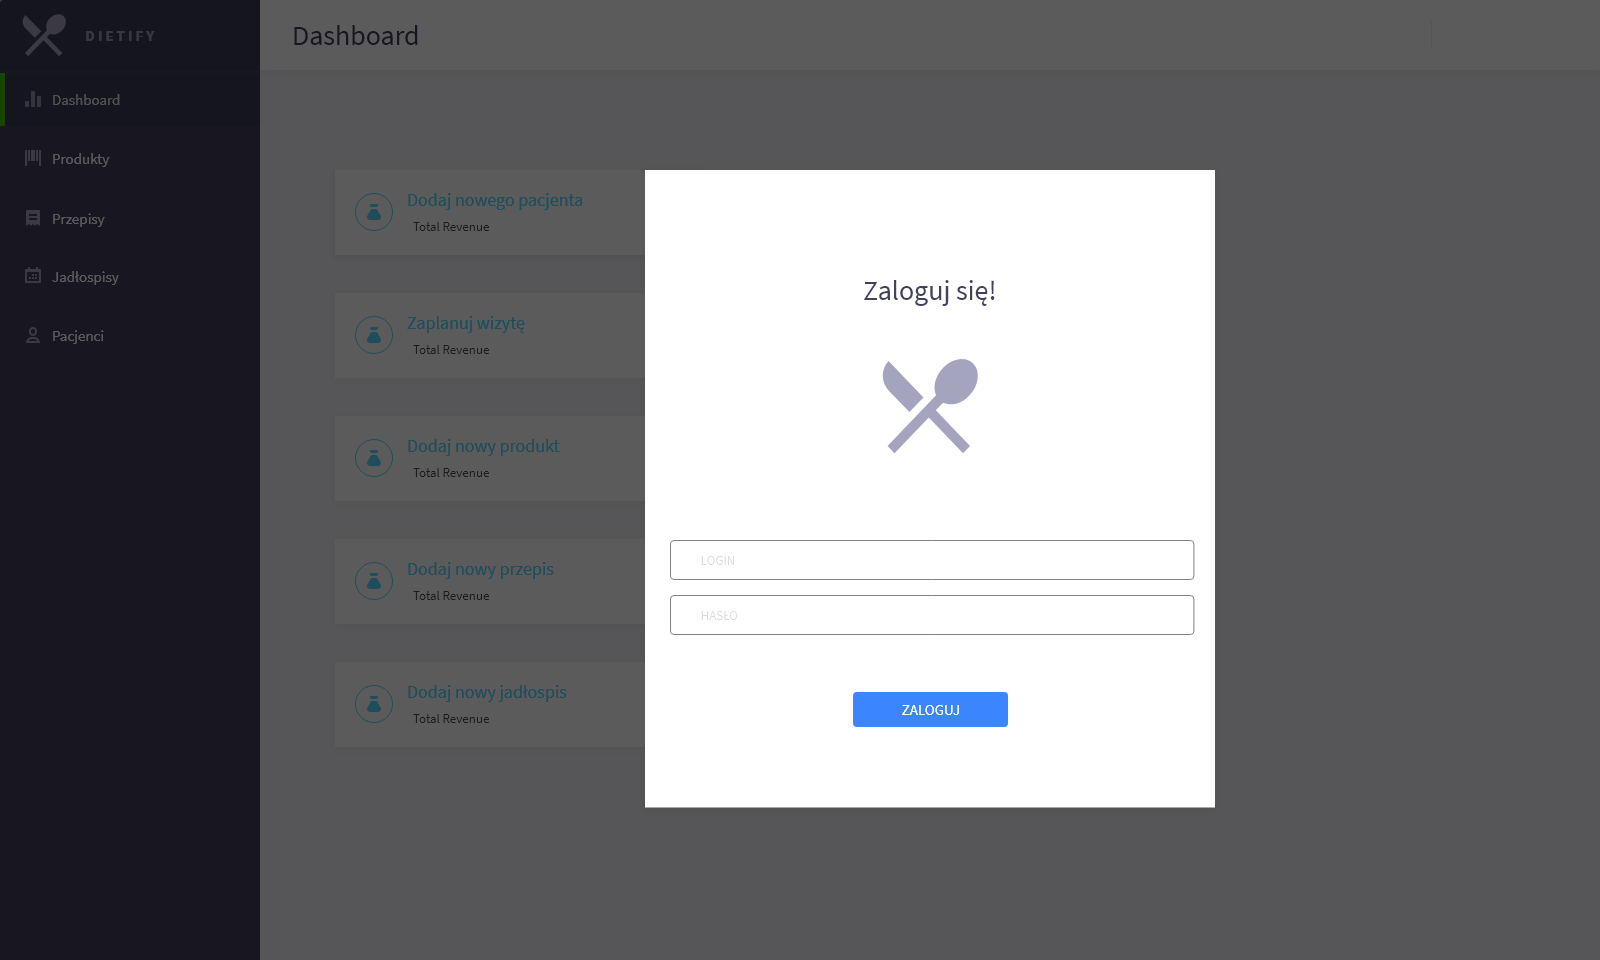
\includegraphics[width=0.9\textwidth]{img/mockups/mockup12.png}
        \caption{Mockup12 (opr.wł).}\label{rysunek:mockup12}
    \end{figure}
\end{minipage}

\begin{minipage}{\textwidth}
    \begin{figure}[H]
        \centering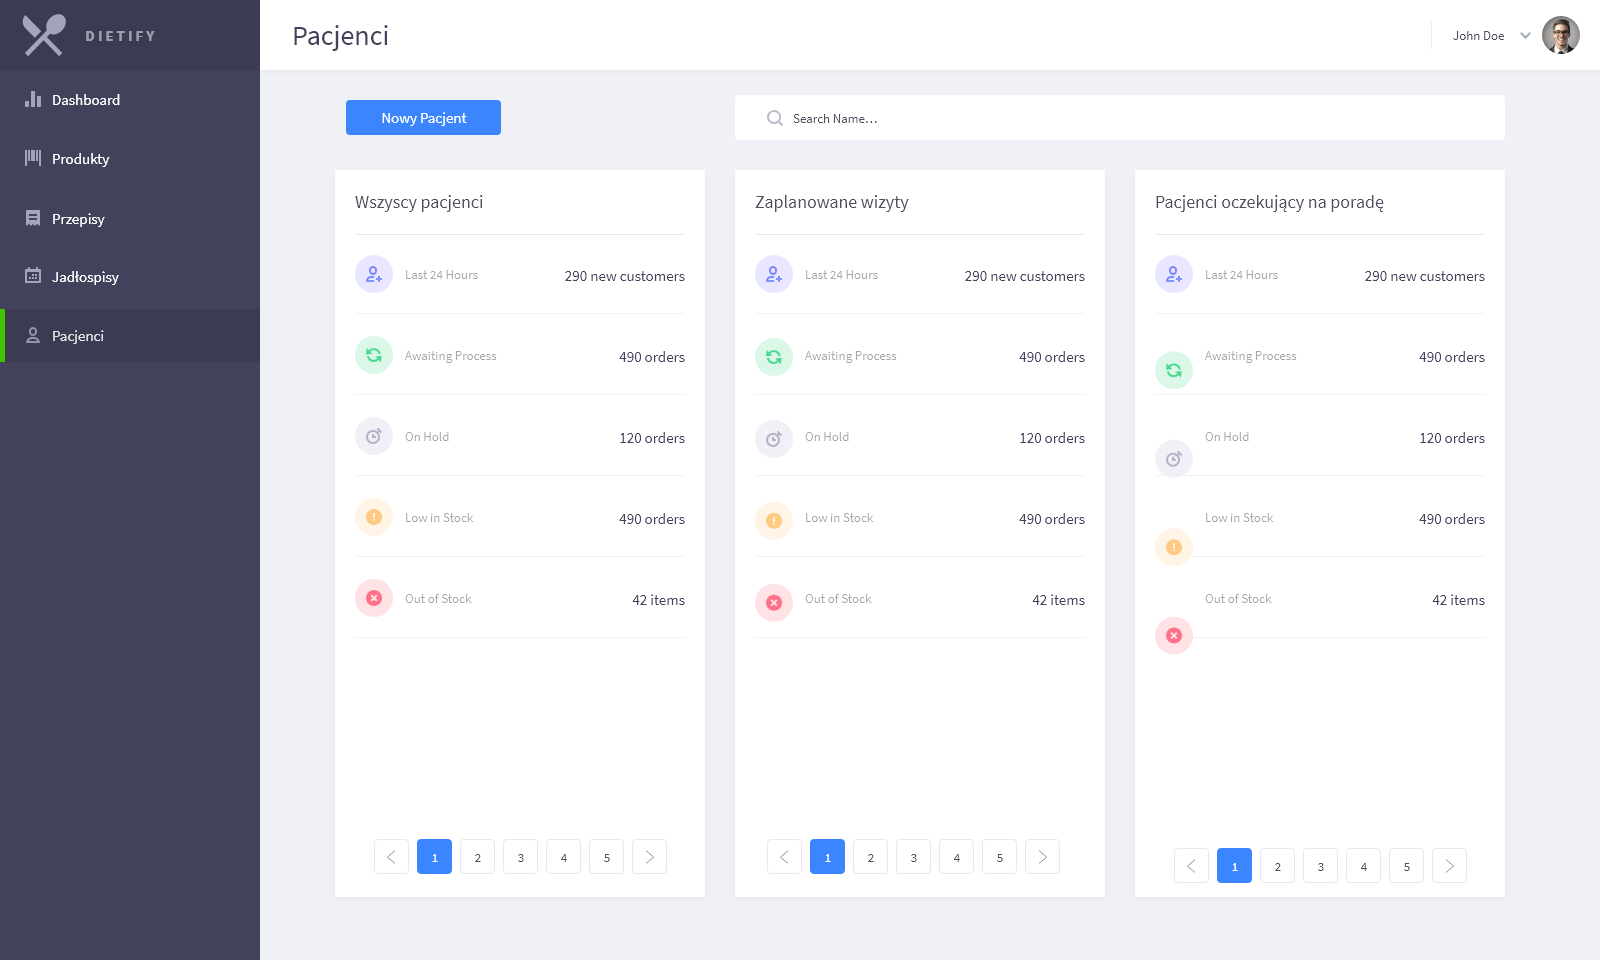
\includegraphics[width=0.9\textwidth]{img/mockups/mockup13.png}
        \caption{Mockup13 (opr.wł).}\label{rysunek:mockup13}
    \end{figure}
\end{minipage}

\begin{minipage}{\textwidth}
    \begin{figure}[H]
        \centering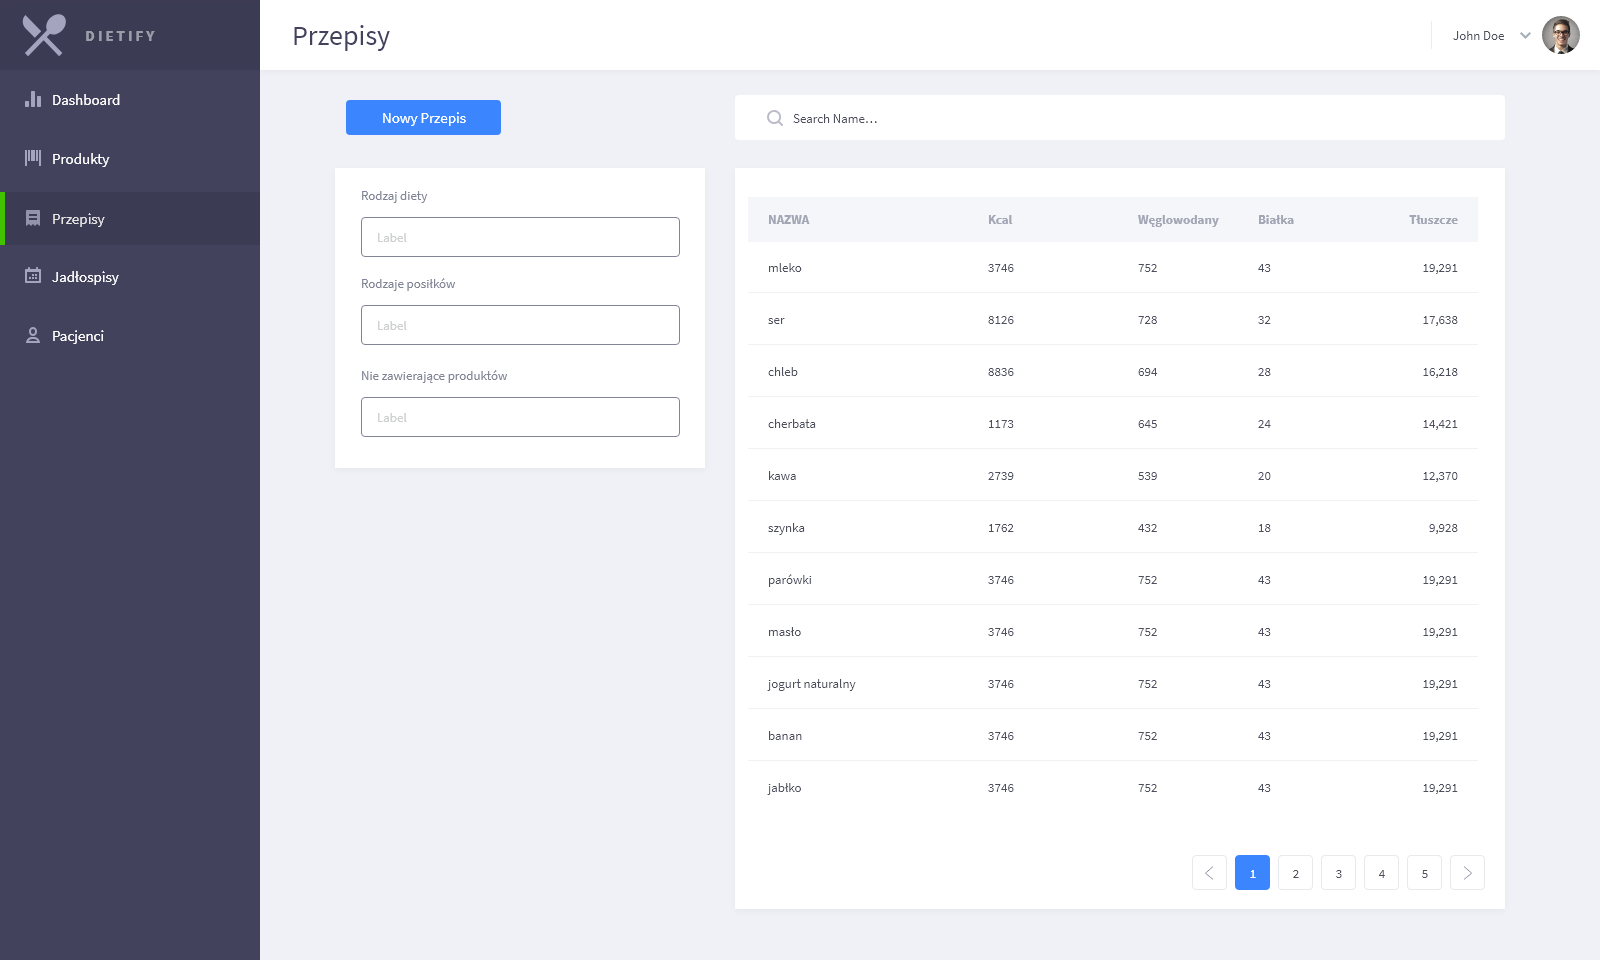
\includegraphics[width=0.9\textwidth]{img/mockups/mockup14.png}
        \caption{Mockup14 (opr.wł).}\label{rysunek:mockup14}
    \end{figure}
\end{minipage}

\begin{minipage}{\textwidth}
    \begin{figure}[H]
        \centering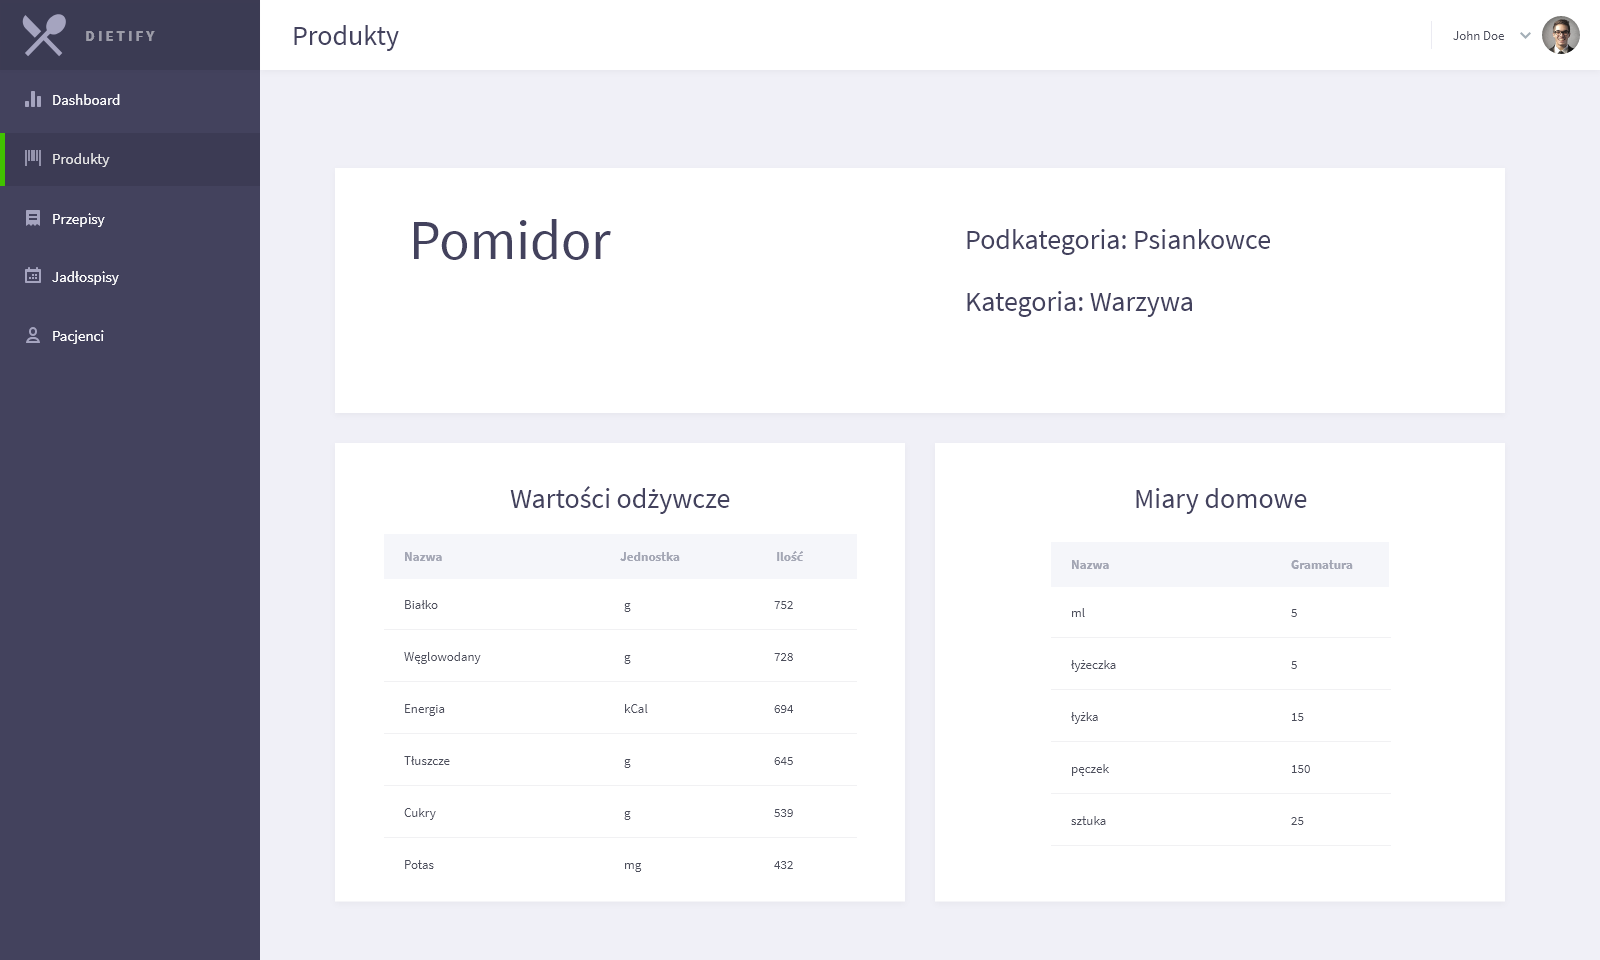
\includegraphics[width=0.9\textwidth]{img/mockups/mockup15.png}
        \caption{Mockup15 (opr.wł).}\label{rysunek:mockup15}
    \end{figure}
\end{minipage}

\begin{minipage}{\textwidth}
    \begin{figure}[H]
        \centering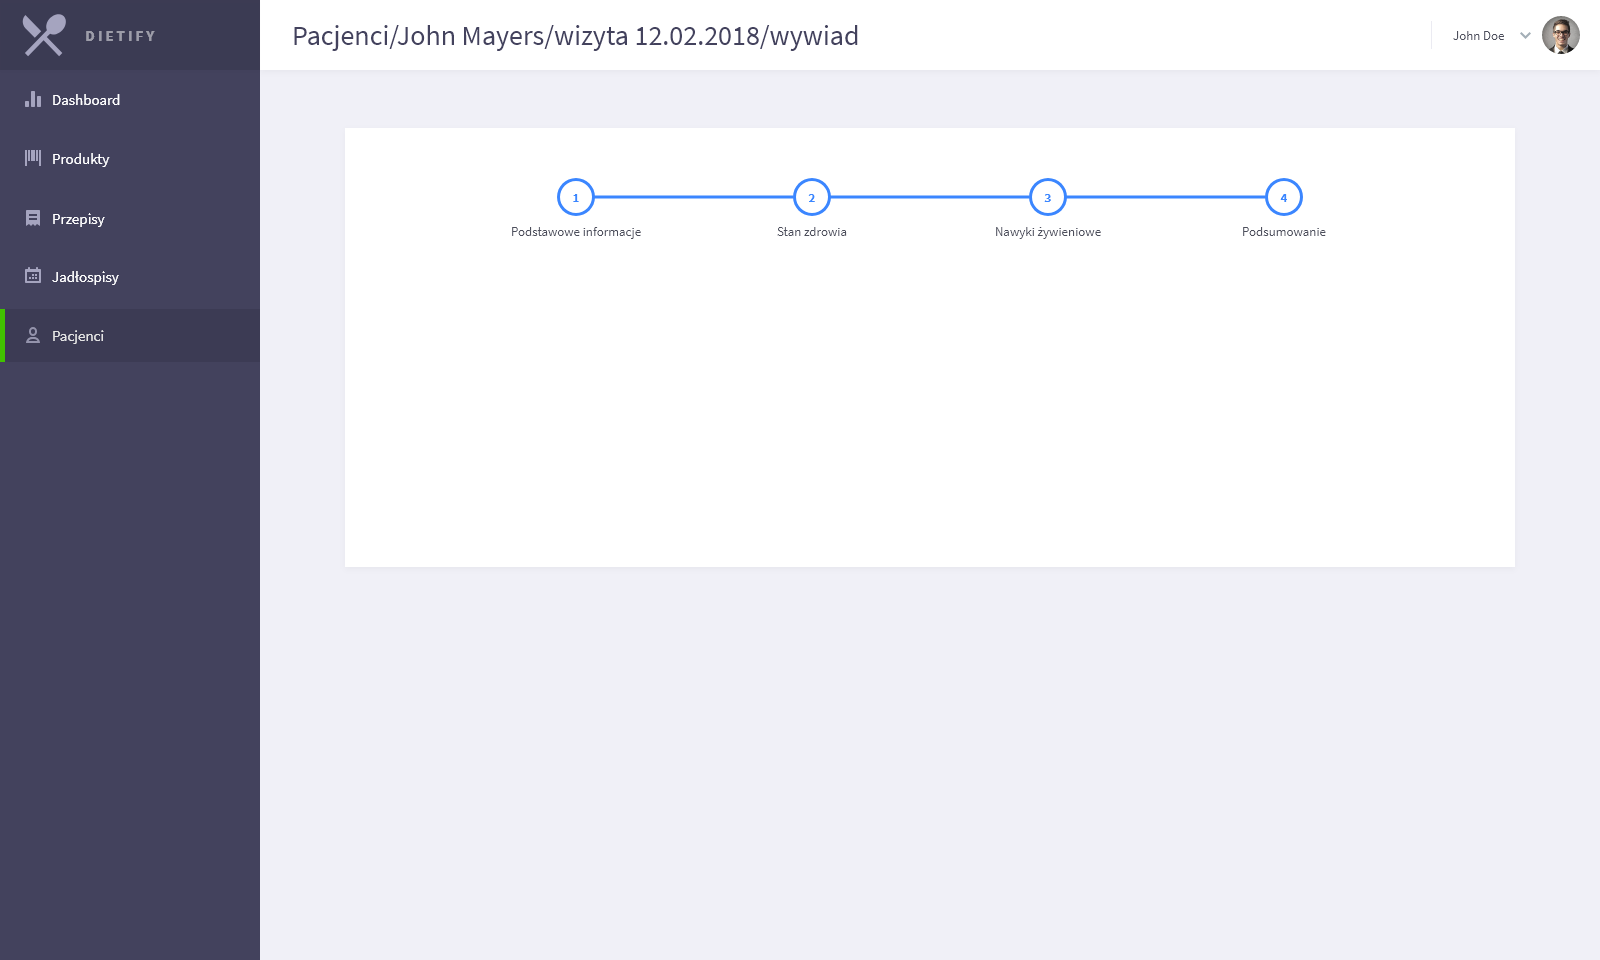
\includegraphics[width=0.9\textwidth]{img/mockups/mockup16.png}
        \caption{Mockup16 (opr.wł).}\label{rysunek:mockup16}
    \end{figure}
\end{minipage}

\section{Baza danych}

\subsection{Kategorie}
\todo{uzupełnić kategorie}

\begin{enumerate}[label={\textbf{KAT/\protect\threedigits{\theenumi}}}, wide, labelwidth=!, labelindent=0pt, series=reqs]
    \setlength\itemsep{1em}
    \req{User} \label{kat:user}

    Opis: \lipsum[1]
    \par
    Atrybuty:
    \begin{itemize}
        \item id
        \item login
        \item passwordHash
        \item firstName
        \item lastName
        \item email
        \item image
        \item activated
        \item langKey
        \item activationKey
        \item createdBy
        \item createdDate
        \item resetDate
        \item lastModifiedBy
        \item lastModifiedDate
    \end{itemize}

    \req{UserExtraInfo} \label{kat:UserExtraInfo}

    Opis: \lipsum[1]
    \par
    Atrybuty:
    \begin{itemize}
        \item id
        \item gender
        \item dateOfBirth
        \item phoneNumber
        \item streetAddress
        \item postalCode
        \item city
        \item country
        \item personalDescription
    \end{itemize}

    \req{SiteContent} \label{kat:SiteContent}

    Opis: \lipsum[1]
    \par
    Atrybuty:
    \begin{itemize}
        \item id
        \item ordinalNumber
        \item siteContentType
        \item title
        \item description
    \end{itemize}

    \req{SiteContentTranslation} \label{kat:SiteContentTranslation}

    Opis: \lipsum[1]
    \par
    Atrybuty:
    \begin{itemize}
        \item id
        \item title
        \item description
        \item language
    \end{itemize}

    \req{ContactInfo} \label{kat:ContactInfo}

    Opis: \lipsum[1]
    \par
    Atrybuty:
    \begin{itemize}
        \item id
        \item contactInfoType
        \item description
    \end{itemize}

    \req{Pricing} \label{kat:Pricing}

    Opis: \lipsum[1]
    \par
    Atrybuty:
    \begin{itemize}
        \item id
        \item ordinalNumber
        \item title
        \item description
        \item price
        \item currency
    \end{itemize}

    \req{PricingTranslation} \label{kat:PricingTranslation}

    Opis: \lipsum[1]
    \par
    Atrybuty:
    \begin{itemize}
        \item id
        \item title
        \item description
        \item language
    \end{itemize}

    \req{Product} \label{kat:Product}

    Opis: \lipsum[1]
    \par
    Atrybuty:
    \begin{itemize}
        \item id
        \item source
        \item isPublic
        \item language
    \end{itemize}

    \req{ProductVersion} \label{kat:ProductVersion}

    Opis: \lipsum[1]
    \par
    Atrybuty:
    \begin{itemize}
        \item id
        \item editTimestamp
        \item description
    \end{itemize}

    \req{ProductBasicNutritionData} \label{kat:ProductBasicNutritionData}

    Opis: \lipsum[1]
    \par
    Atrybuty:
    \begin{itemize}
        \item id
        \item energy
        \item protein
        \item fat
        \item carbohydrates
    \end{itemize}

    \req{NutritionData} \label{kat:NutritionData}

    Opis: \lipsum[1]
    \par
    Atrybuty:
    \begin{itemize}
        \item id
        \item nutritionValue
    \end{itemize}

    \req{NutritionDefinition} \label{kat:NutritionDefinition}

    Opis: \lipsum[1]
    \par
    Atrybuty:
    \begin{itemize}
        \item id
        \item tag
        \item description
        \item units
        \item decimalPlaces
    \end{itemize}

    \req{NutritionDefinitionTranslation} \label{kat:NutritionDefinitionTranslation}

    Opis: \lipsum[1]
    \par
    Atrybuty:
    \begin{itemize}
        \item id
        \item translation
        \item language
    \end{itemize}

    \req{HouseholdMeasure} \label{kat:HouseholdMeasure}

    Opis: \lipsum[1]
    \par
    Atrybuty:
    \begin{itemize}
        \item id
        \item description
        \item gramsWeight
        \item isVisible
    \end{itemize}

    \req{ProductSubcategory} \label{kat:ProductSubcategory}

    Opis: \lipsum[1]
    \par
    Atrybuty:
    \begin{itemize}
        \item id
        \item description
    \end{itemize}

    \req{ProductCategory} \label{kat:ProductCategory}

    Opis: \lipsum[1]
    \par
    Atrybuty:
    \begin{itemize}
        \item id
        \item description
    \end{itemize}

    \req{ProductCategoryTranslation} \label{kat:ProductCategoryTranslation}

    Opis: \lipsum[1]
    \par
    Atrybuty:
    \begin{itemize}
        \item id
        \item translation
        \item language
    \end{itemize}

    \req{DietType} \label{kat:DietType}

    Opis: \lipsum[1]
    \par
    Atrybuty:
    \begin{itemize}
        \item id
        \item name
    \end{itemize}

    \req{DietTypeTranslation} \label{kat:DietTypeTranslation}

    Opis: \lipsum[1]
    \par
    Atrybuty:
    \begin{itemize}
        \item id
        \item translation
        \item language
    \end{itemize}

    \req{Recipe} \label{kat:Recipe}

    Opis: \lipsum[1]
    \par
    Atrybuty:
    \begin{itemize}
        \item id
        \item isPublic
        \item language
    \end{itemize}

    \req{RecipeVersion} \label{kat:RecipeVersion}

    Opis: \lipsum[1]
    \par
    Atrybuty:
    \begin{itemize}
        \item id
        \item editTimestamp
        \item name
        \item preparationTimeMinutes
        \item numberOfPortions
        \item image
        \item totalGramsWeight
    \end{itemize}

    \req{RecipeBasicNutritionData} \label{kat:RecipeBasicNutritionData}

    Opis: \lipsum[1]
    \par
    Atrybuty:
    \begin{itemize}
        \item id
        \item energy
        \item protein
        \item fat
        \item carbohydrates
    \end{itemize}

    \req{RecipeSection} \label{kat:RecipeSection}

    Opis: \lipsum[1]
    \par
    Atrybuty:
    \begin{itemize}
        \item id
        \item sectionName
    \end{itemize}

    \req{ProductPortion} \label{kat:ProductPortion}

    Opis: \lipsum[1]
    \par
    Atrybuty:
    \begin{itemize}
        \item id
        \item amount
    \end{itemize}

    \req{PreparationStep} \label{kat:PreparationStep}

    Opis: \lipsum[1]
    \par
    Atrybuty:
    \begin{itemize}
        \item id
        \item ordinalNumber
        \item stepDescription
    \end{itemize}

    \req{KitchenAppliance} \label{kat:KitchenAppliance}

    Opis: \lipsum[1]
    \par
    Atrybuty:
    \begin{itemize}
        \item id
        \item name
    \end{itemize}

    \req{KitchenApplianceTranslation} \label{kat:KitchenApplianceTranslation}

    Opis: \lipsum[1]
    \par
    Atrybuty:
    \begin{itemize}
        \item id
        \item translation
        \item language
    \end{itemize}

    \req{DishType} \label{kat:DishType}

    Opis: \lipsum[1]
    \par
    Atrybuty:
    \begin{itemize}
        \item id
        \item description
    \end{itemize}

    \req{DishTypeTranslation} \label{kat:DishTypeTranslation}

    Opis: \lipsum[1]
    \par
    Atrybuty:
    \begin{itemize}
        \item id
        \item translation
        \item language
    \end{itemize}

    \req{MealType} \label{kat:MealType}

    Opis: \lipsum[1]
    \par
    Atrybuty:
    \begin{itemize}
        \item id
        \item name
    \end{itemize}

    \req{MealTypeTranslation} \label{kat:MealTypeTranslation}

    Opis: \lipsum[1]
    \par
    Atrybuty:
    \begin{itemize}
        \item id
        \item translation
        \item language
    \end{itemize}


    \req{MealPlan} \label{kat:MealPlan}

    Opis: \lipsum[1]
    \par
    Atrybuty:
    \begin{itemize}
        \item id
        \item creationTimestamp
        \item editTimestamp
        \item name
        \item isVisible
        \item language
        \item numberOfDays
        \item numberOfMealsPerDay
        \item totalDailyEnergy
        \item percentOfProtein
        \item percentOfFat
        \item percentOfCarbohydrates
    \end{itemize}

    \req{MealPlanDay} \label{kat:MealPlanDay}

    Opis: \lipsum[1]
    \par
    Atrybuty:
    \begin{itemize}
        \item id
        \item ordinalNumber
    \end{itemize}

    \req{Meal} \label{kat:Meal}

    Opis: \lipsum[1]
    \par
    Atrybuty:
    \begin{itemize}
        \item id
        \item ordinalNumber
    \end{itemize}

    \req{MealRecipe} \label{kat:MealRecipe}

    Opis: \lipsum[1]
    \par
    Atrybuty:
    \begin{itemize}
        \item id
        \item amount
    \end{itemize}

    \req{MealProduct} \label{kat:MealProduct}

    Opis: \lipsum[1]
    \par
    Atrybuty:
    \begin{itemize}
        \item id
        \item amount
    \end{itemize}

    \req{MealDefinition} \label{kat:MealDefinition}

    Opis: \lipsum[1]
    \par
    Atrybuty:
    \begin{itemize}
        \item id
        \item ordinalNumber
        \item timeOfMeal
        \item percentOfEnergy
    \end{itemize}

    \req{Appointment} \label{kat:Appointment}

    Opis: \lipsum[1]
    \par
    Atrybuty:
    \begin{itemize}
        \item id
        \item appointmentDate
        \item appointmentState
        \item generalAdvice
    \end{itemize}

    \req{PatientCard} \label{kat:PatientCard}

    Opis: \lipsum[1]
    \par
    Atrybuty:
    \begin{itemize}
        \item id
        \item creationDate
    \end{itemize}

    \req{AppointmentEvaluation} \label{kat:AppointmentEvaluation}

    Opis: \lipsum[1]
    \par
    Atrybuty:
    \begin{itemize}
        \item id
        \item overallSatisfaction
        \item dietitianServiceSatisfaction
        \item mealPlanOverallSatisfaction
        \item mealCostSatisfaction
        \item mealPreparationTimeSatisfaction
        \item mealComplexityLevelSatisfaction
        \item mealTastefulnessSatisfaction
        \item dietaryResultSatisfaction
        \item comment
    \end{itemize}

    \req{BodyMeasurement} \label{kat:BodyMeasurement}

    Opis: \lipsum[1]
    \par
    Atrybuty:
    \begin{itemize}
        \item id
        \item completionDate
        \item height
        \item weight
        \item waist
        \item percentOfFatTissue
        \item percentOfWater
        \item muscleMass
        \item physicalMark
        \item calciumInBones
        \item basicMetabolism
        \item metabolicAge
        \item visceralDatLevel
    \end{itemize}

    \req{NutritionalInterview} \label{kat:NutritionalInterview}

    Opis: \lipsum[1]
    \par
    Atrybuty:
    \begin{itemize}
        \item id
        \item completionDate
        \item targetWeight
        \item advicePurpose
        \item physicalActivity
        \item diseases
        \item medicines
        \item jobType
        \item likedProducts
        \item dislikedProducts
        \item foodAllergies
        \item foodIntolerances
    \end{itemize}

    \req{OwnedKitchenAppliance} \label{kat:OwnedKitchenAppliance}

    Opis: \lipsum[1]
    \par
    Atrybuty:
    \begin{itemize}
        \item id
    \end{itemize}

    \req{CustomNutritionalInterviewQuestion} \label{kat:CustomNutritionalInterviewQuestion}

    Opis: \lipsum[1]
    \par
    Atrybuty:
    \begin{itemize}
        \item id
        \item ordinalNumber
        \item question
        \item answer
    \end{itemize}

    \req{CustomNutritionalInterviewQuestionTemplate} \label{kat:CustomNutritionalInterviewQuestionTemplate}

    Opis: \lipsum[1]
    \par
    Atrybuty:
    \begin{itemize}
        \item id
        \item question
        \item language
    \end{itemize}

    \req{AssignedMealPlan} \label{kat:AssignedMealPlan}

    Opis: \lipsum[1]
    \par
    Atrybuty:
    \begin{itemize}
        \item id
        \item assigmentTime
    \end{itemize}


\end{enumerate}

\subsection {Reguły funkcjonowania}
\todo{uzupełnić reguły funkcjonowania, i.e. związki pomiędzy encjami}

\begin{itemize}[label={\textbf{Reguły dla}}, wide, labelwidth=!, labelindent=0pt]
    \setlength\itemsep{1em}
    \item\ref{kat:user}
    \begin{enumerate}[label={\textbf{REG/\protect\threedigits{\arabic{enumi}}}}, wide, labelwidth=!]
        \item test1
        \item test2
    \end{enumerate}
    \item\ref{kat:UserExtraInfo}
    \begin{enumerate}[label={\textbf{REG/\protect\threedigits{\arabic{enumi}}}}, wide, labelwidth=!, resume]
        \item test1
        \item test2
    \end{enumerate}
    \item\ref{kat:SiteContent}
    \begin{enumerate}[label={\textbf{REG/\protect\threedigits{\arabic{enumi}}}}, wide, labelwidth=!, resume]
        \item test1
        \item test2
    \end{enumerate}
    \item\ref{kat:SiteContentTranslation}
    \begin{enumerate}[label={\textbf{REG/\protect\threedigits{\arabic{enumi}}}}, wide, labelwidth=!, resume]
        \item test1
        \item test2
    \end{enumerate}
    \item\ref{kat:ContactInfo}
    \begin{enumerate}[label={\textbf{REG/\protect\threedigits{\arabic{enumi}}}}, wide, labelwidth=!, resume]
        \item test1
        \item test2
    \end{enumerate}
    \item\ref{kat:Pricing}
    \begin{enumerate}[label={\textbf{REG/\protect\threedigits{\arabic{enumi}}}}, wide, labelwidth=!, resume]
        \item test1
        \item test2
    \end{enumerate}
    \item\ref{kat:PricingTranslation}
    \begin{enumerate}[label={\textbf{REG/\protect\threedigits{\arabic{enumi}}}}, wide, labelwidth=!, resume]
        \item test1
        \item test2
    \end{enumerate}
    \item\ref{kat:Product}
    \begin{enumerate}[label={\textbf{REG/\protect\threedigits{\arabic{enumi}}}}, wide, labelwidth=!, resume]
        \item test1
        \item test2
    \end{enumerate}
    \item\ref{kat:ProductVersion}
    \begin{enumerate}[label={\textbf{REG/\protect\threedigits{\arabic{enumi}}}}, wide, labelwidth=!, resume]
        \item test1
        \item test2
    \end{enumerate}
    \item\ref{kat:ProductBasicNutritionData}
    \begin{enumerate}[label={\textbf{REG/\protect\threedigits{\arabic{enumi}}}}, wide, labelwidth=!, resume]
        \item test1
        \item test2
    \end{enumerate}
    \item\ref{kat:NutritionData}
    \begin{enumerate}[label={\textbf{REG/\protect\threedigits{\arabic{enumi}}}}, wide, labelwidth=!, resume]
        \item test1
        \item test2
    \end{enumerate}
    \item\ref{kat:NutritionDefinition}
    \begin{enumerate}[label={\textbf{REG/\protect\threedigits{\arabic{enumi}}}}, wide, labelwidth=!, resume]
        \item test1
        \item test2
    \end{enumerate}
    \item\ref{kat:NutritionDefinitionTranslation}
    \begin{enumerate}[label={\textbf{REG/\protect\threedigits{\arabic{enumi}}}}, wide, labelwidth=!, resume]
        \item test1
        \item test2
    \end{enumerate}
    \item\ref{kat:HouseholdMeasure}
    \begin{enumerate}[label={\textbf{REG/\protect\threedigits{\arabic{enumi}}}}, wide, labelwidth=!, resume]
        \item test1
        \item test2
    \end{enumerate}
    \item\ref{kat:ProductSubcategory}
    \begin{enumerate}[label={\textbf{REG/\protect\threedigits{\arabic{enumi}}}}, wide, labelwidth=!, resume]
        \item test1
        \item test2
    \end{enumerate}
    \item\ref{kat:ProductCategory}
    \begin{enumerate}[label={\textbf{REG/\protect\threedigits{\arabic{enumi}}}}, wide, labelwidth=!, resume]
        \item test1
        \item test2
    \end{enumerate}
    \item\ref{kat:ProductCategoryTranslation}
    \begin{enumerate}[label={\textbf{REG/\protect\threedigits{\arabic{enumi}}}}, wide, labelwidth=!, resume]
        \item test1
        \item test2
    \end{enumerate}
    \item\ref{kat:DietType}
    \begin{enumerate}[label={\textbf{REG/\protect\threedigits{\arabic{enumi}}}}, wide, labelwidth=!, resume]
        \item test1
        \item test2
    \end{enumerate}
    \item\ref{kat:DietTypeTranslation}
    \begin{enumerate}[label={\textbf{REG/\protect\threedigits{\arabic{enumi}}}}, wide, labelwidth=!, resume]
        \item test1
        \item test2
    \end{enumerate}
    \item\ref{kat:Recipe}
    \begin{enumerate}[label={\textbf{REG/\protect\threedigits{\arabic{enumi}}}}, wide, labelwidth=!, resume]
        \item test1
        \item test2
    \end{enumerate}
    \item\ref{kat:RecipeVersion}
    \begin{enumerate}[label={\textbf{REG/\protect\threedigits{\arabic{enumi}}}}, wide, labelwidth=!, resume]
        \item test1
        \item test2
    \end{enumerate}
    \item\ref{kat:RecipeBasicNutritionData}
    \begin{enumerate}[label={\textbf{REG/\protect\threedigits{\arabic{enumi}}}}, wide, labelwidth=!, resume]
        \item test1
        \item test2
    \end{enumerate}
    \item\ref{kat:RecipeSection}
    \begin{enumerate}[label={\textbf{REG/\protect\threedigits{\arabic{enumi}}}}, wide, labelwidth=!, resume]
        \item test1
        \item test2
    \end{enumerate}
    \item\ref{kat:ProductPortion}
    \begin{enumerate}[label={\textbf{REG/\protect\threedigits{\arabic{enumi}}}}, wide, labelwidth=!, resume]
        \item test1
        \item test2
    \end{enumerate}
    \item\ref{kat:PreparationStep}
    \begin{enumerate}[label={\textbf{REG/\protect\threedigits{\arabic{enumi}}}}, wide, labelwidth=!, resume]
        \item test1
        \item test2
    \end{enumerate}
    \item\ref{kat:KitchenAppliance}
    \begin{enumerate}[label={\textbf{REG/\protect\threedigits{\arabic{enumi}}}}, wide, labelwidth=!, resume]
        \item test1
        \item test2
    \end{enumerate}
    \item\ref{kat:KitchenApplianceTranslation}
    \begin{enumerate}[label={\textbf{REG/\protect\threedigits{\arabic{enumi}}}}, wide, labelwidth=!, resume]
        \item test1
        \item test2
    \end{enumerate}
    \item\ref{kat:DishType}
    \begin{enumerate}[label={\textbf{REG/\protect\threedigits{\arabic{enumi}}}}, wide, labelwidth=!, resume]
        \item test1
        \item test2
    \end{enumerate}
    \item\ref{kat:DishTypeTranslation}
    \begin{enumerate}[label={\textbf{REG/\protect\threedigits{\arabic{enumi}}}}, wide, labelwidth=!, resume]
        \item test1
        \item test2
    \end{enumerate}
    \item\ref{kat:MealType}
    \begin{enumerate}[label={\textbf{REG/\protect\threedigits{\arabic{enumi}}}}, wide, labelwidth=!, resume]
        \item test1
        \item test2
    \end{enumerate}
    \item\ref{kat:MealTypeTranslation}
    \begin{enumerate}[label={\textbf{REG/\protect\threedigits{\arabic{enumi}}}}, wide, labelwidth=!, resume]
        \item test1
        \item test2
    \end{enumerate}
    \item\ref{kat:MealPlan}
    \begin{enumerate}[label={\textbf{REG/\protect\threedigits{\arabic{enumi}}}}, wide, labelwidth=!, resume]
        \item test1
        \item test2
    \end{enumerate}
    \item\ref{kat:MealPlanDay}
    \begin{enumerate}[label={\textbf{REG/\protect\threedigits{\arabic{enumi}}}}, wide, labelwidth=!, resume]
        \item test1
        \item test2
    \end{enumerate}
    \item\ref{kat:Meal}
    \begin{enumerate}[label={\textbf{REG/\protect\threedigits{\arabic{enumi}}}}, wide, labelwidth=!, resume]
        \item test1
        \item test2
    \end{enumerate}
    \item\ref{kat:MealRecipe}
    \begin{enumerate}[label={\textbf{REG/\protect\threedigits{\arabic{enumi}}}}, wide, labelwidth=!, resume]
        \item test1
        \item test2
    \end{enumerate}
    \item\ref{kat:MealProduct}
    \begin{enumerate}[label={\textbf{REG/\protect\threedigits{\arabic{enumi}}}}, wide, labelwidth=!, resume]
        \item test1
        \item test2
    \end{enumerate}
    \item\ref{kat:MealDefinition}
    \begin{enumerate}[label={\textbf{REG/\protect\threedigits{\arabic{enumi}}}}, wide, labelwidth=!, resume]
        \item test1
        \item test2
    \end{enumerate}
    \item\ref{kat:Appointment}
    \begin{enumerate}[label={\textbf{REG/\protect\threedigits{\arabic{enumi}}}}, wide, labelwidth=!, resume]
        \item test1
        \item test2
    \end{enumerate}
    \item\ref{kat:PatientCard}
    \begin{enumerate}[label={\textbf{REG/\protect\threedigits{\arabic{enumi}}}}, wide, labelwidth=!, resume]
        \item test1
        \item test2
    \end{enumerate}
    \item\ref{kat:AppointmentEvaluation}
    \begin{enumerate}[label={\textbf{REG/\protect\threedigits{\arabic{enumi}}}}, wide, labelwidth=!, resume]
        \item test1
        \item test2
    \end{enumerate}
    \item\ref{kat:BodyMeasurement}
    \begin{enumerate}[label={\textbf{REG/\protect\threedigits{\arabic{enumi}}}}, wide, labelwidth=!, resume]
        \item test1
        \item test2
    \end{enumerate}
    \item\ref{kat:NutritionalInterview}
    \begin{enumerate}[label={\textbf{REG/\protect\threedigits{\arabic{enumi}}}}, wide, labelwidth=!, resume]
        \item test1
        \item test2
    \end{enumerate}
    \item\ref{kat:OwnedKitchenAppliance}
    \begin{enumerate}[label={\textbf{REG/\protect\threedigits{\arabic{enumi}}}}, wide, labelwidth=!, resume]
        \item test1
        \item test2
    \end{enumerate}
    \item\ref{kat:CustomNutritionalInterviewQuestion}
    \begin{enumerate}[label={\textbf{REG/\protect\threedigits{\arabic{enumi}}}}, wide, labelwidth=!, resume]
        \item test1
        \item test2
    \end{enumerate}
    \item\ref{kat:CustomNutritionalInterviewQuestionTemplate}
    \begin{enumerate}[label={\textbf{REG/\protect\threedigits{\arabic{enumi}}}}, wide, labelwidth=!, resume]
        \item test1
        \item test2
    \end{enumerate}
    \item\ref{kat:AssignedMealPlan}
    \begin{enumerate}[label={\textbf{REG/\protect\threedigits{\arabic{enumi}}}}, wide, labelwidth=!, resume]
        \item test1
        \item test2
    \end{enumerate}
\end{itemize}

\subsection{Ograniczenia dziedzinowe}
\todo{uzupełnić ograniczenia dziedzionowe}

\begin{itemize}[label={\textbf{Ograniczenia dla}}, wide, labelwidth=!, labelindent=0pt]
    \setlength\itemsep{1em}
    \item\ref{kat:user}
    \begin{enumerate}[label={\textbf{OGR/\protect\threedigits{\arabic{enumi}}}}, wide, labelwidth=!]
        \item test1
        \item test2
    \end{enumerate}
    \item\ref{kat:UserExtraInfo}
    \begin{enumerate}[label={\textbf{OGR/\protect\threedigits{\arabic{enumi}}}}, wide, labelwidth=!, resume]
        \item test1
        \item test2
    \end{enumerate}
    \item\ref{kat:SiteContent}
    \begin{enumerate}[label={\textbf{OGR/\protect\threedigits{\arabic{enumi}}}}, wide, labelwidth=!, resume]
        \item test1
        \item test2
    \end{enumerate}
    \item\ref{kat:SiteContentTranslation}
    \begin{enumerate}[label={\textbf{OGR/\protect\threedigits{\arabic{enumi}}}}, wide, labelwidth=!, resume]
        \item test1
        \item test2
    \end{enumerate}
    \item\ref{kat:ContactInfo}
    \begin{enumerate}[label={\textbf{OGR/\protect\threedigits{\arabic{enumi}}}}, wide, labelwidth=!, resume]
        \item test1
        \item test2
    \end{enumerate}
    \item\ref{kat:Pricing}
    \begin{enumerate}[label={\textbf{OGR/\protect\threedigits{\arabic{enumi}}}}, wide, labelwidth=!, resume]
        \item test1
        \item test2
    \end{enumerate}
    \item\ref{kat:PricingTranslation}
    \begin{enumerate}[label={\textbf{OGR/\protect\threedigits{\arabic{enumi}}}}, wide, labelwidth=!, resume]
        \item test1
        \item test2
    \end{enumerate}
    \item\ref{kat:Product}
    \begin{enumerate}[label={\textbf{OGR/\protect\threedigits{\arabic{enumi}}}}, wide, labelwidth=!, resume]
        \item test1
        \item test2
    \end{enumerate}
    \item\ref{kat:ProductVersion}
    \begin{enumerate}[label={\textbf{OGR/\protect\threedigits{\arabic{enumi}}}}, wide, labelwidth=!, resume]
        \item test1
        \item test2
    \end{enumerate}
    \item\ref{kat:ProductBasicNutritionData}
    \begin{enumerate}[label={\textbf{OGR/\protect\threedigits{\arabic{enumi}}}}, wide, labelwidth=!, resume]
        \item test1
        \item test2
    \end{enumerate}
    \item\ref{kat:NutritionData}
    \begin{enumerate}[label={\textbf{OGR/\protect\threedigits{\arabic{enumi}}}}, wide, labelwidth=!, resume]
        \item test1
        \item test2
    \end{enumerate}
    \item\ref{kat:NutritionDefinition}
    \begin{enumerate}[label={\textbf{OGR/\protect\threedigits{\arabic{enumi}}}}, wide, labelwidth=!, resume]
        \item test1
        \item test2
    \end{enumerate}
    \item\ref{kat:NutritionDefinitionTranslation}
    \begin{enumerate}[label={\textbf{OGR/\protect\threedigits{\arabic{enumi}}}}, wide, labelwidth=!, resume]
        \item test1
        \item test2
    \end{enumerate}
    \item\ref{kat:HouseholdMeasure}
    \begin{enumerate}[label={\textbf{OGR/\protect\threedigits{\arabic{enumi}}}}, wide, labelwidth=!, resume]
        \item test1
        \item test2
    \end{enumerate}
    \item\ref{kat:ProductSubcategory}
    \begin{enumerate}[label={\textbf{OGR/\protect\threedigits{\arabic{enumi}}}}, wide, labelwidth=!, resume]
        \item test1
        \item test2
    \end{enumerate}
    \item\ref{kat:ProductCategory}
    \begin{enumerate}[label={\textbf{OGR/\protect\threedigits{\arabic{enumi}}}}, wide, labelwidth=!, resume]
        \item test1
        \item test2
    \end{enumerate}
    \item\ref{kat:ProductCategoryTranslation}
    \begin{enumerate}[label={\textbf{OGR/\protect\threedigits{\arabic{enumi}}}}, wide, labelwidth=!, resume]
        \item test1
        \item test2
    \end{enumerate}
    \item\ref{kat:DietType}
    \begin{enumerate}[label={\textbf{OGR/\protect\threedigits{\arabic{enumi}}}}, wide, labelwidth=!, resume]
        \item test1
        \item test2
    \end{enumerate}
    \item\ref{kat:DietTypeTranslation}
    \begin{enumerate}[label={\textbf{OGR/\protect\threedigits{\arabic{enumi}}}}, wide, labelwidth=!, resume]
        \item test1
        \item test2
    \end{enumerate}
    \item\ref{kat:Recipe}
    \begin{enumerate}[label={\textbf{OGR/\protect\threedigits{\arabic{enumi}}}}, wide, labelwidth=!, resume]
        \item test1
        \item test2
    \end{enumerate}
    \item\ref{kat:RecipeVersion}
    \begin{enumerate}[label={\textbf{OGR/\protect\threedigits{\arabic{enumi}}}}, wide, labelwidth=!, resume]
        \item test1
        \item test2
    \end{enumerate}
    \item\ref{kat:RecipeBasicNutritionData}
    \begin{enumerate}[label={\textbf{OGR/\protect\threedigits{\arabic{enumi}}}}, wide, labelwidth=!, resume]
        \item test1
        \item test2
    \end{enumerate}
    \item\ref{kat:RecipeSection}
    \begin{enumerate}[label={\textbf{OGR/\protect\threedigits{\arabic{enumi}}}}, wide, labelwidth=!, resume]
        \item test1
        \item test2
    \end{enumerate}
    \item\ref{kat:ProductPortion}
    \begin{enumerate}[label={\textbf{OGR/\protect\threedigits{\arabic{enumi}}}}, wide, labelwidth=!, resume]
        \item test1
        \item test2
    \end{enumerate}
    \item\ref{kat:PreparationStep}
    \begin{enumerate}[label={\textbf{OGR/\protect\threedigits{\arabic{enumi}}}}, wide, labelwidth=!, resume]
        \item test1
        \item test2
    \end{enumerate}
    \item\ref{kat:KitchenAppliance}
    \begin{enumerate}[label={\textbf{OGR/\protect\threedigits{\arabic{enumi}}}}, wide, labelwidth=!, resume]
        \item test1
        \item test2
    \end{enumerate}
    \item\ref{kat:KitchenApplianceTranslation}
    \begin{enumerate}[label={\textbf{OGR/\protect\threedigits{\arabic{enumi}}}}, wide, labelwidth=!, resume]
        \item test1
        \item test2
    \end{enumerate}
    \item\ref{kat:DishType}
    \begin{enumerate}[label={\textbf{OGR/\protect\threedigits{\arabic{enumi}}}}, wide, labelwidth=!, resume]
        \item test1
        \item test2
    \end{enumerate}
    \item\ref{kat:DishTypeTranslation}
    \begin{enumerate}[label={\textbf{OGR/\protect\threedigits{\arabic{enumi}}}}, wide, labelwidth=!, resume]
        \item test1
        \item test2
    \end{enumerate}
    \item\ref{kat:MealType}
    \begin{enumerate}[label={\textbf{OGR/\protect\threedigits{\arabic{enumi}}}}, wide, labelwidth=!, resume]
        \item test1
        \item test2
    \end{enumerate}
    \item\ref{kat:MealTypeTranslation}
    \begin{enumerate}[label={\textbf{OGR/\protect\threedigits{\arabic{enumi}}}}, wide, labelwidth=!, resume]
        \item test1
        \item test2
    \end{enumerate}
    \item\ref{kat:MealPlan}
    \begin{enumerate}[label={\textbf{OGR/\protect\threedigits{\arabic{enumi}}}}, wide, labelwidth=!, resume]
        \item test1
        \item test2
    \end{enumerate}
    \item\ref{kat:MealPlanDay}
    \begin{enumerate}[label={\textbf{OGR/\protect\threedigits{\arabic{enumi}}}}, wide, labelwidth=!, resume]
        \item test1
        \item test2
    \end{enumerate}
    \item\ref{kat:Meal}
    \begin{enumerate}[label={\textbf{OGR/\protect\threedigits{\arabic{enumi}}}}, wide, labelwidth=!, resume]
        \item test1
        \item test2
    \end{enumerate}
    \item\ref{kat:MealRecipe}
    \begin{enumerate}[label={\textbf{OGR/\protect\threedigits{\arabic{enumi}}}}, wide, labelwidth=!, resume]
        \item test1
        \item test2
    \end{enumerate}
    \item\ref{kat:MealProduct}
    \begin{enumerate}[label={\textbf{OGR/\protect\threedigits{\arabic{enumi}}}}, wide, labelwidth=!, resume]
        \item test1
        \item test2
    \end{enumerate}
    \item\ref{kat:MealDefinition}
    \begin{enumerate}[label={\textbf{OGR/\protect\threedigits{\arabic{enumi}}}}, wide, labelwidth=!, resume]
        \item test1
        \item test2
    \end{enumerate}
    \item\ref{kat:Appointment}
    \begin{enumerate}[label={\textbf{OGR/\protect\threedigits{\arabic{enumi}}}}, wide, labelwidth=!, resume]
        \item test1
        \item test2
    \end{enumerate}
    \item\ref{kat:PatientCard}
    \begin{enumerate}[label={\textbf{OGR/\protect\threedigits{\arabic{enumi}}}}, wide, labelwidth=!, resume]
        \item test1
        \item test2
    \end{enumerate}
    \item\ref{kat:AppointmentEvaluation}
    \begin{enumerate}[label={\textbf{OGR/\protect\threedigits{\arabic{enumi}}}}, wide, labelwidth=!, resume]
        \item test1
        \item test2
    \end{enumerate}
    \item\ref{kat:BodyMeasurement}
    \begin{enumerate}[label={\textbf{OGR/\protect\threedigits{\arabic{enumi}}}}, wide, labelwidth=!, resume]
        \item test1
        \item test2
    \end{enumerate}
    \item\ref{kat:NutritionalInterview}
    \begin{enumerate}[label={\textbf{OGR/\protect\threedigits{\arabic{enumi}}}}, wide, labelwidth=!, resume]
        \item test1
        \item test2
    \end{enumerate}
    \item\ref{kat:OwnedKitchenAppliance}
    \begin{enumerate}[label={\textbf{OGR/\protect\threedigits{\arabic{enumi}}}}, wide, labelwidth=!, resume]
        \item test1
        \item test2
    \end{enumerate}
    \item\ref{kat:CustomNutritionalInterviewQuestion}
    \begin{enumerate}[label={\textbf{OGR/\protect\threedigits{\arabic{enumi}}}}, wide, labelwidth=!, resume]
        \item test1
        \item test2
    \end{enumerate}
    \item\ref{kat:CustomNutritionalInterviewQuestionTemplate}
    \begin{enumerate}[label={\textbf{OGR/\protect\threedigits{\arabic{enumi}}}}, wide, labelwidth=!, resume]
        \item test1
        \item test2
    \end{enumerate}
    \item\ref{kat:AssignedMealPlan}
    \begin{enumerate}[label={\textbf{OGR/\protect\threedigits{\arabic{enumi}}}}, wide, labelwidth=!, resume]
        \item test1
        \item test2
    \end{enumerate}
\end{itemize}

\section{Model domenowy}
\todo{diagram klas}

\begin{minipage}{\textwidth}
    \begin{figure}[H]
        \centering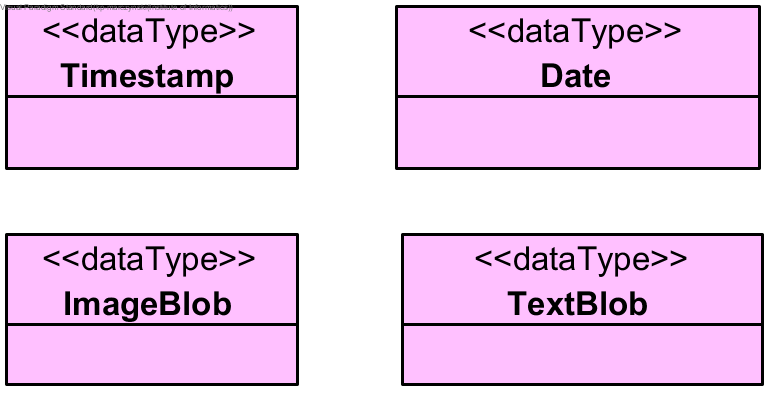
\includegraphics[scale=0.7]{../uml/class_diagrams/dataTypes.png}
        \caption{Typy danych - diagram klas (opr.wł).}\label{rysunek:class-diagram-data-types}
    \end{figure}
\end{minipage}

\begin{minipage}{\textwidth}
    \begin{figure}[H]
        \centering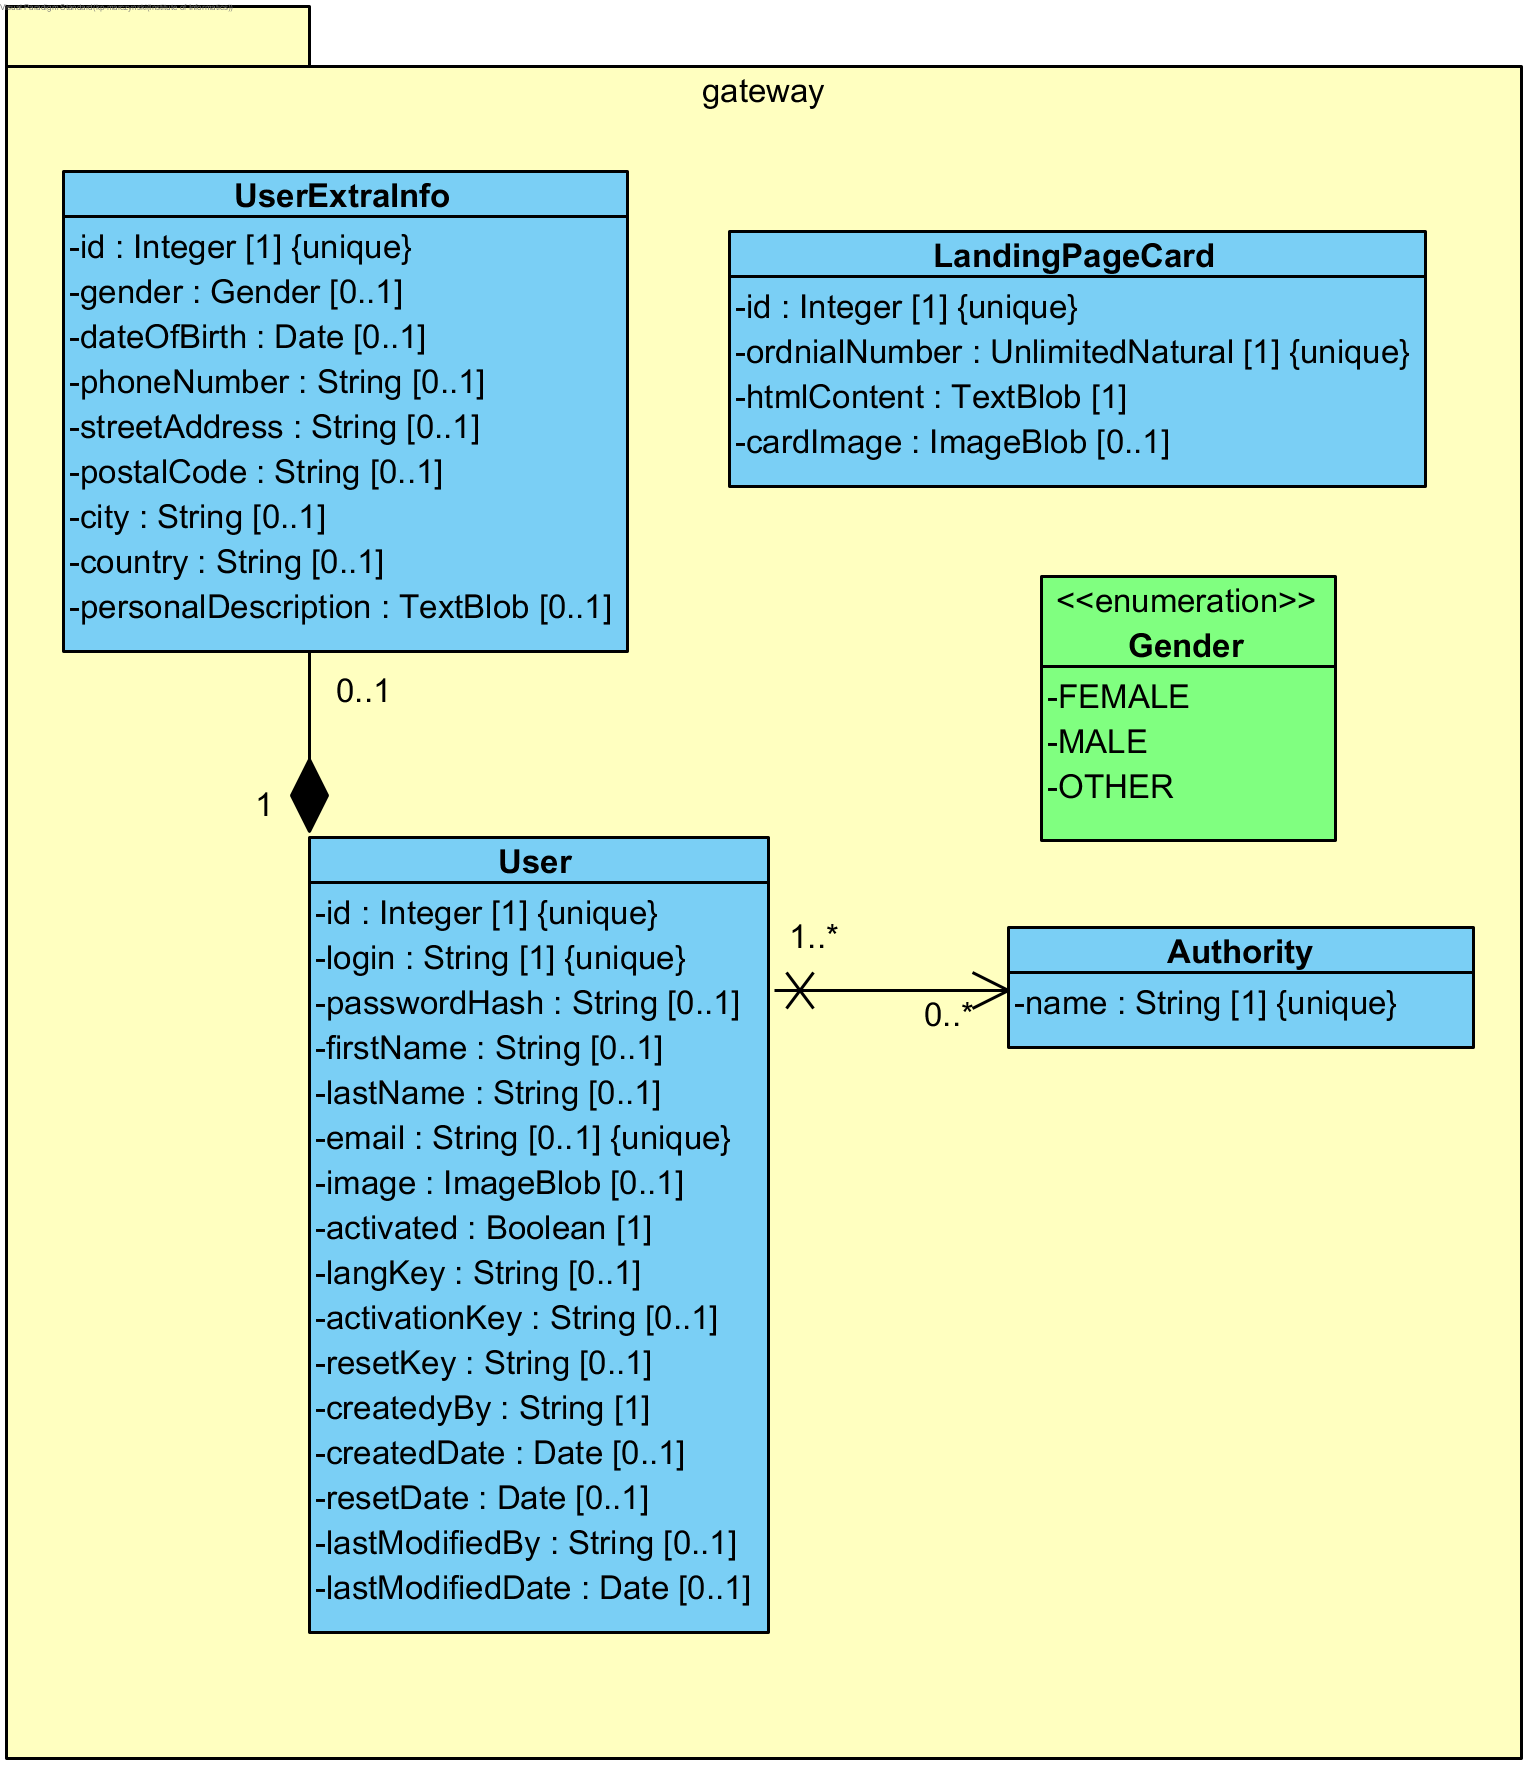
\includegraphics[scale=0.7]{../uml/class_diagrams/gateway.png}
        \caption{Gateway - diagram klas (opr.wł).}\label{rysunek:class-diagram-gateway}
    \end{figure}
\end{minipage}

\begin{minipage}{\textwidth}
    \begin{figure}[H]
        \centering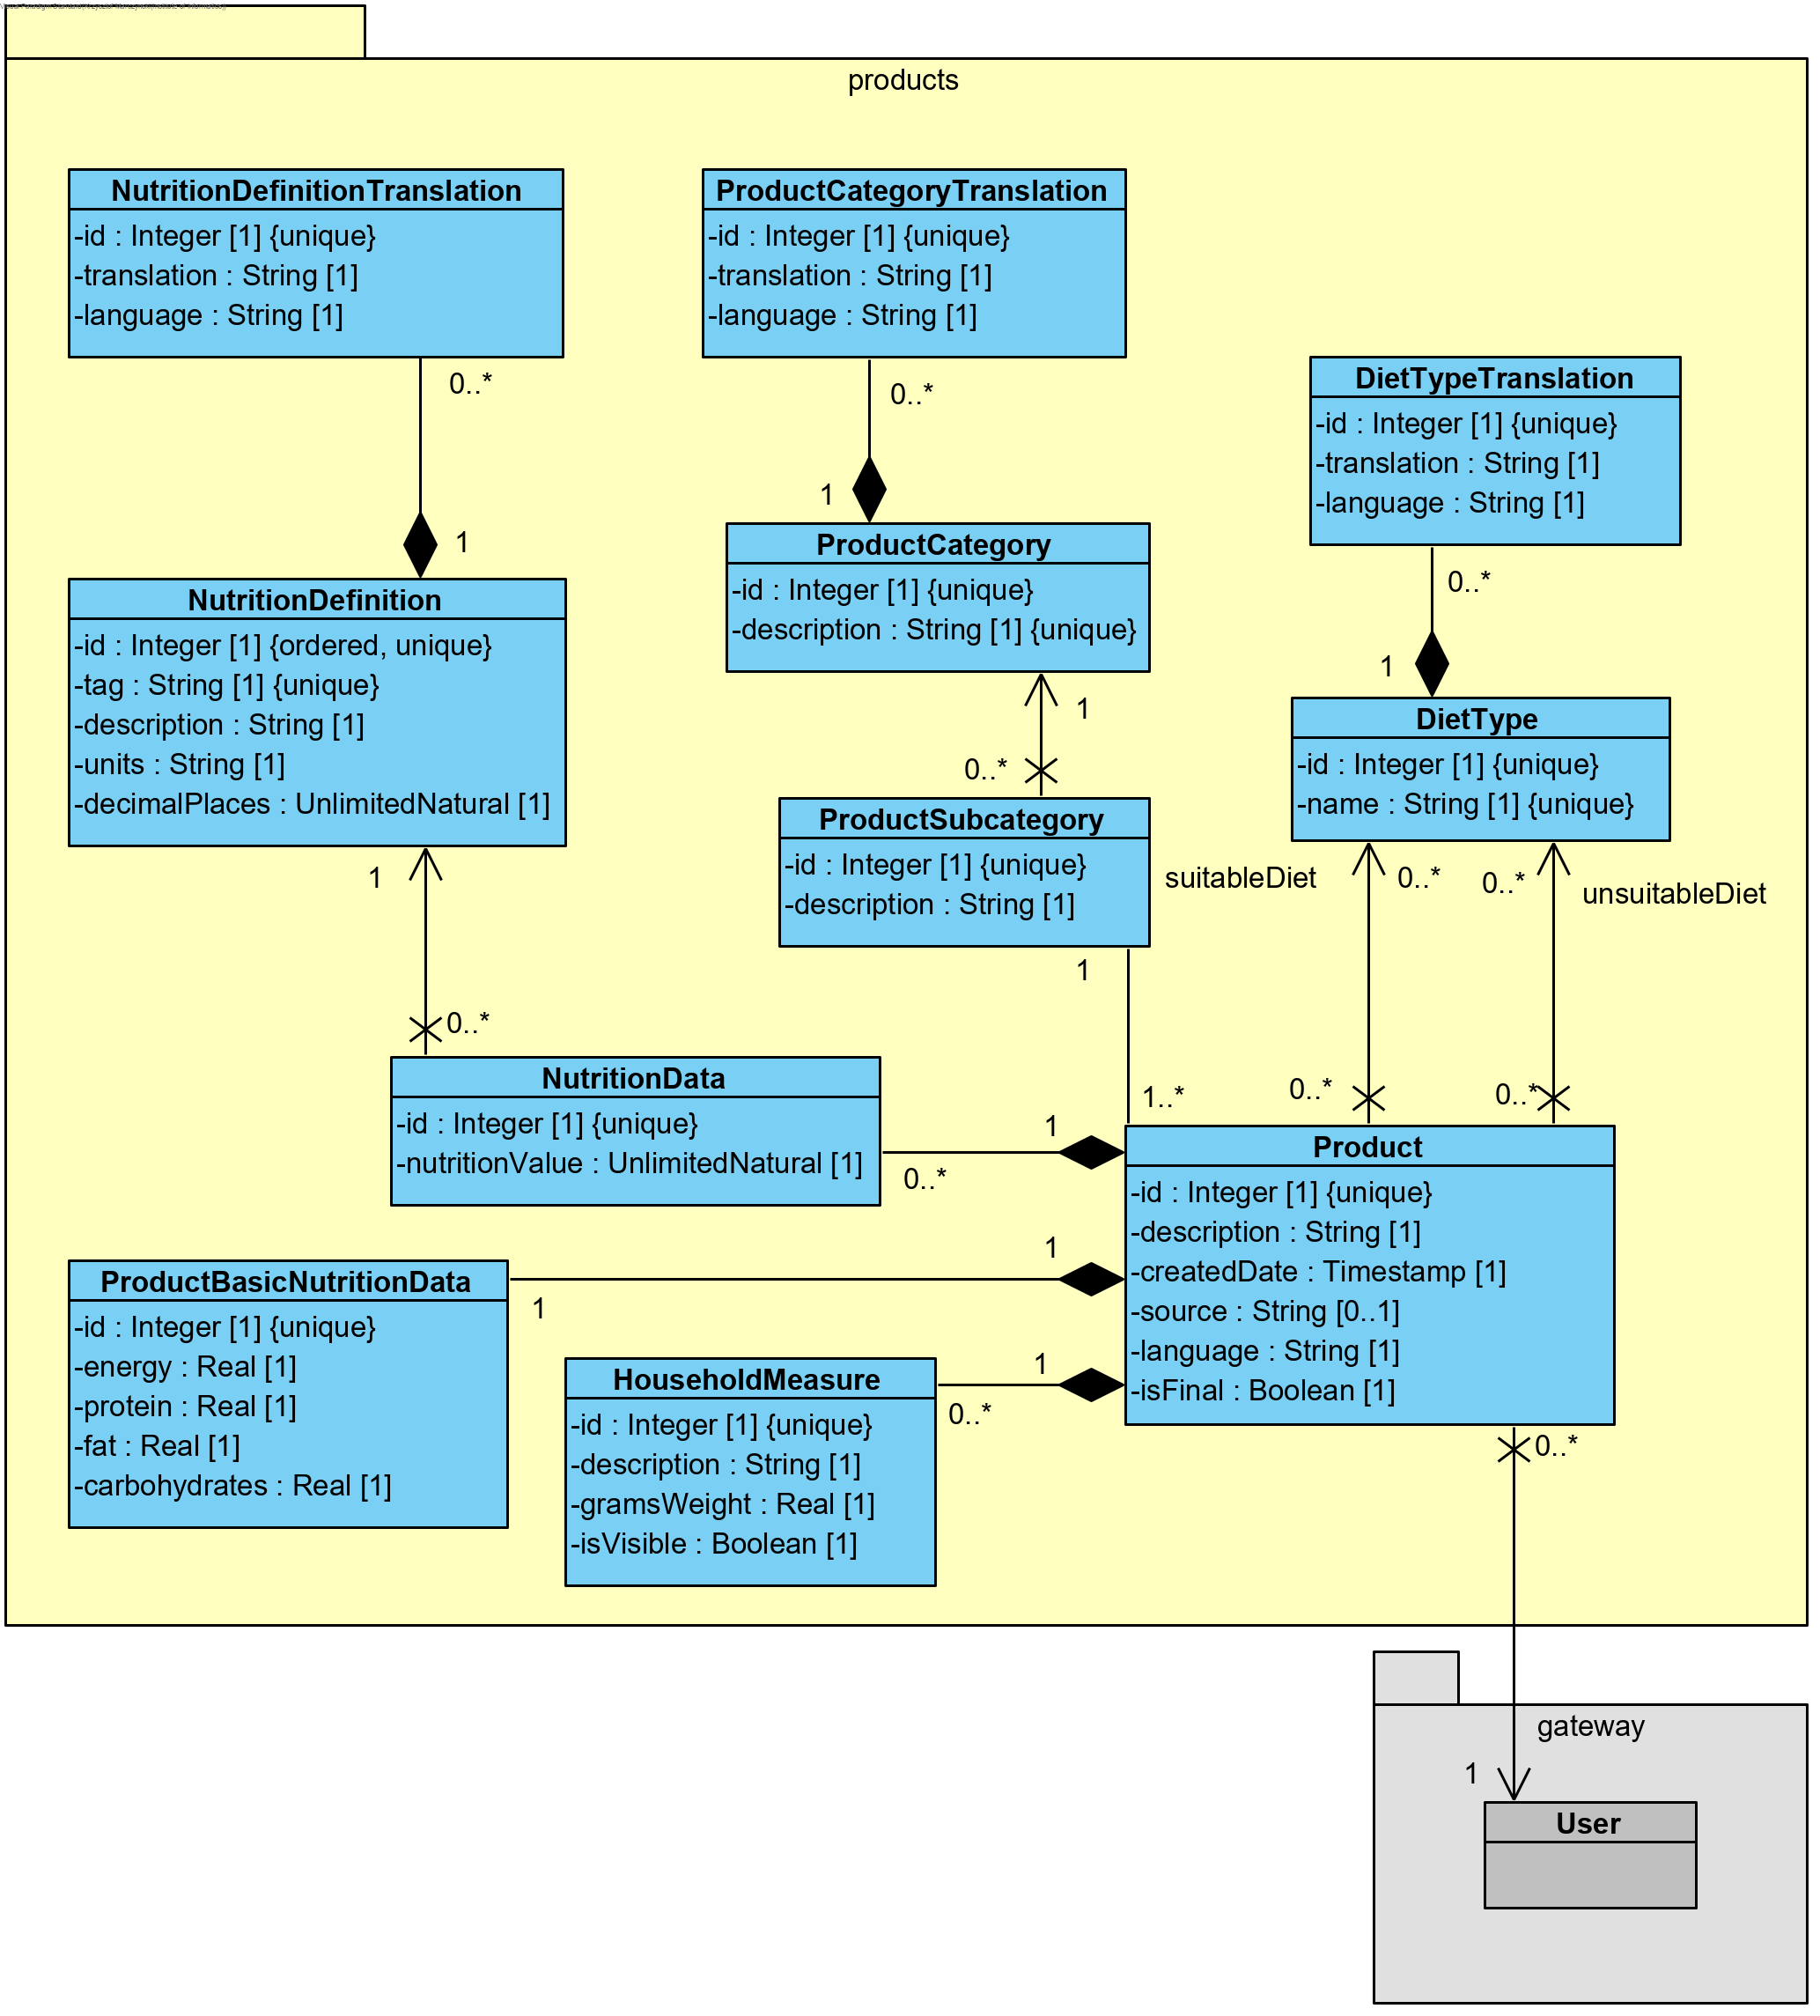
\includegraphics[scale=0.7]{../uml/class_diagrams/products.png}
        \caption{Produkty - diagram klas (opr.wł).}\label{rysunek:class-diagram-products}
    \end{figure}
\end{minipage}

\begin{minipage}{\textwidth}
    \begin{figure}[H]
        \centering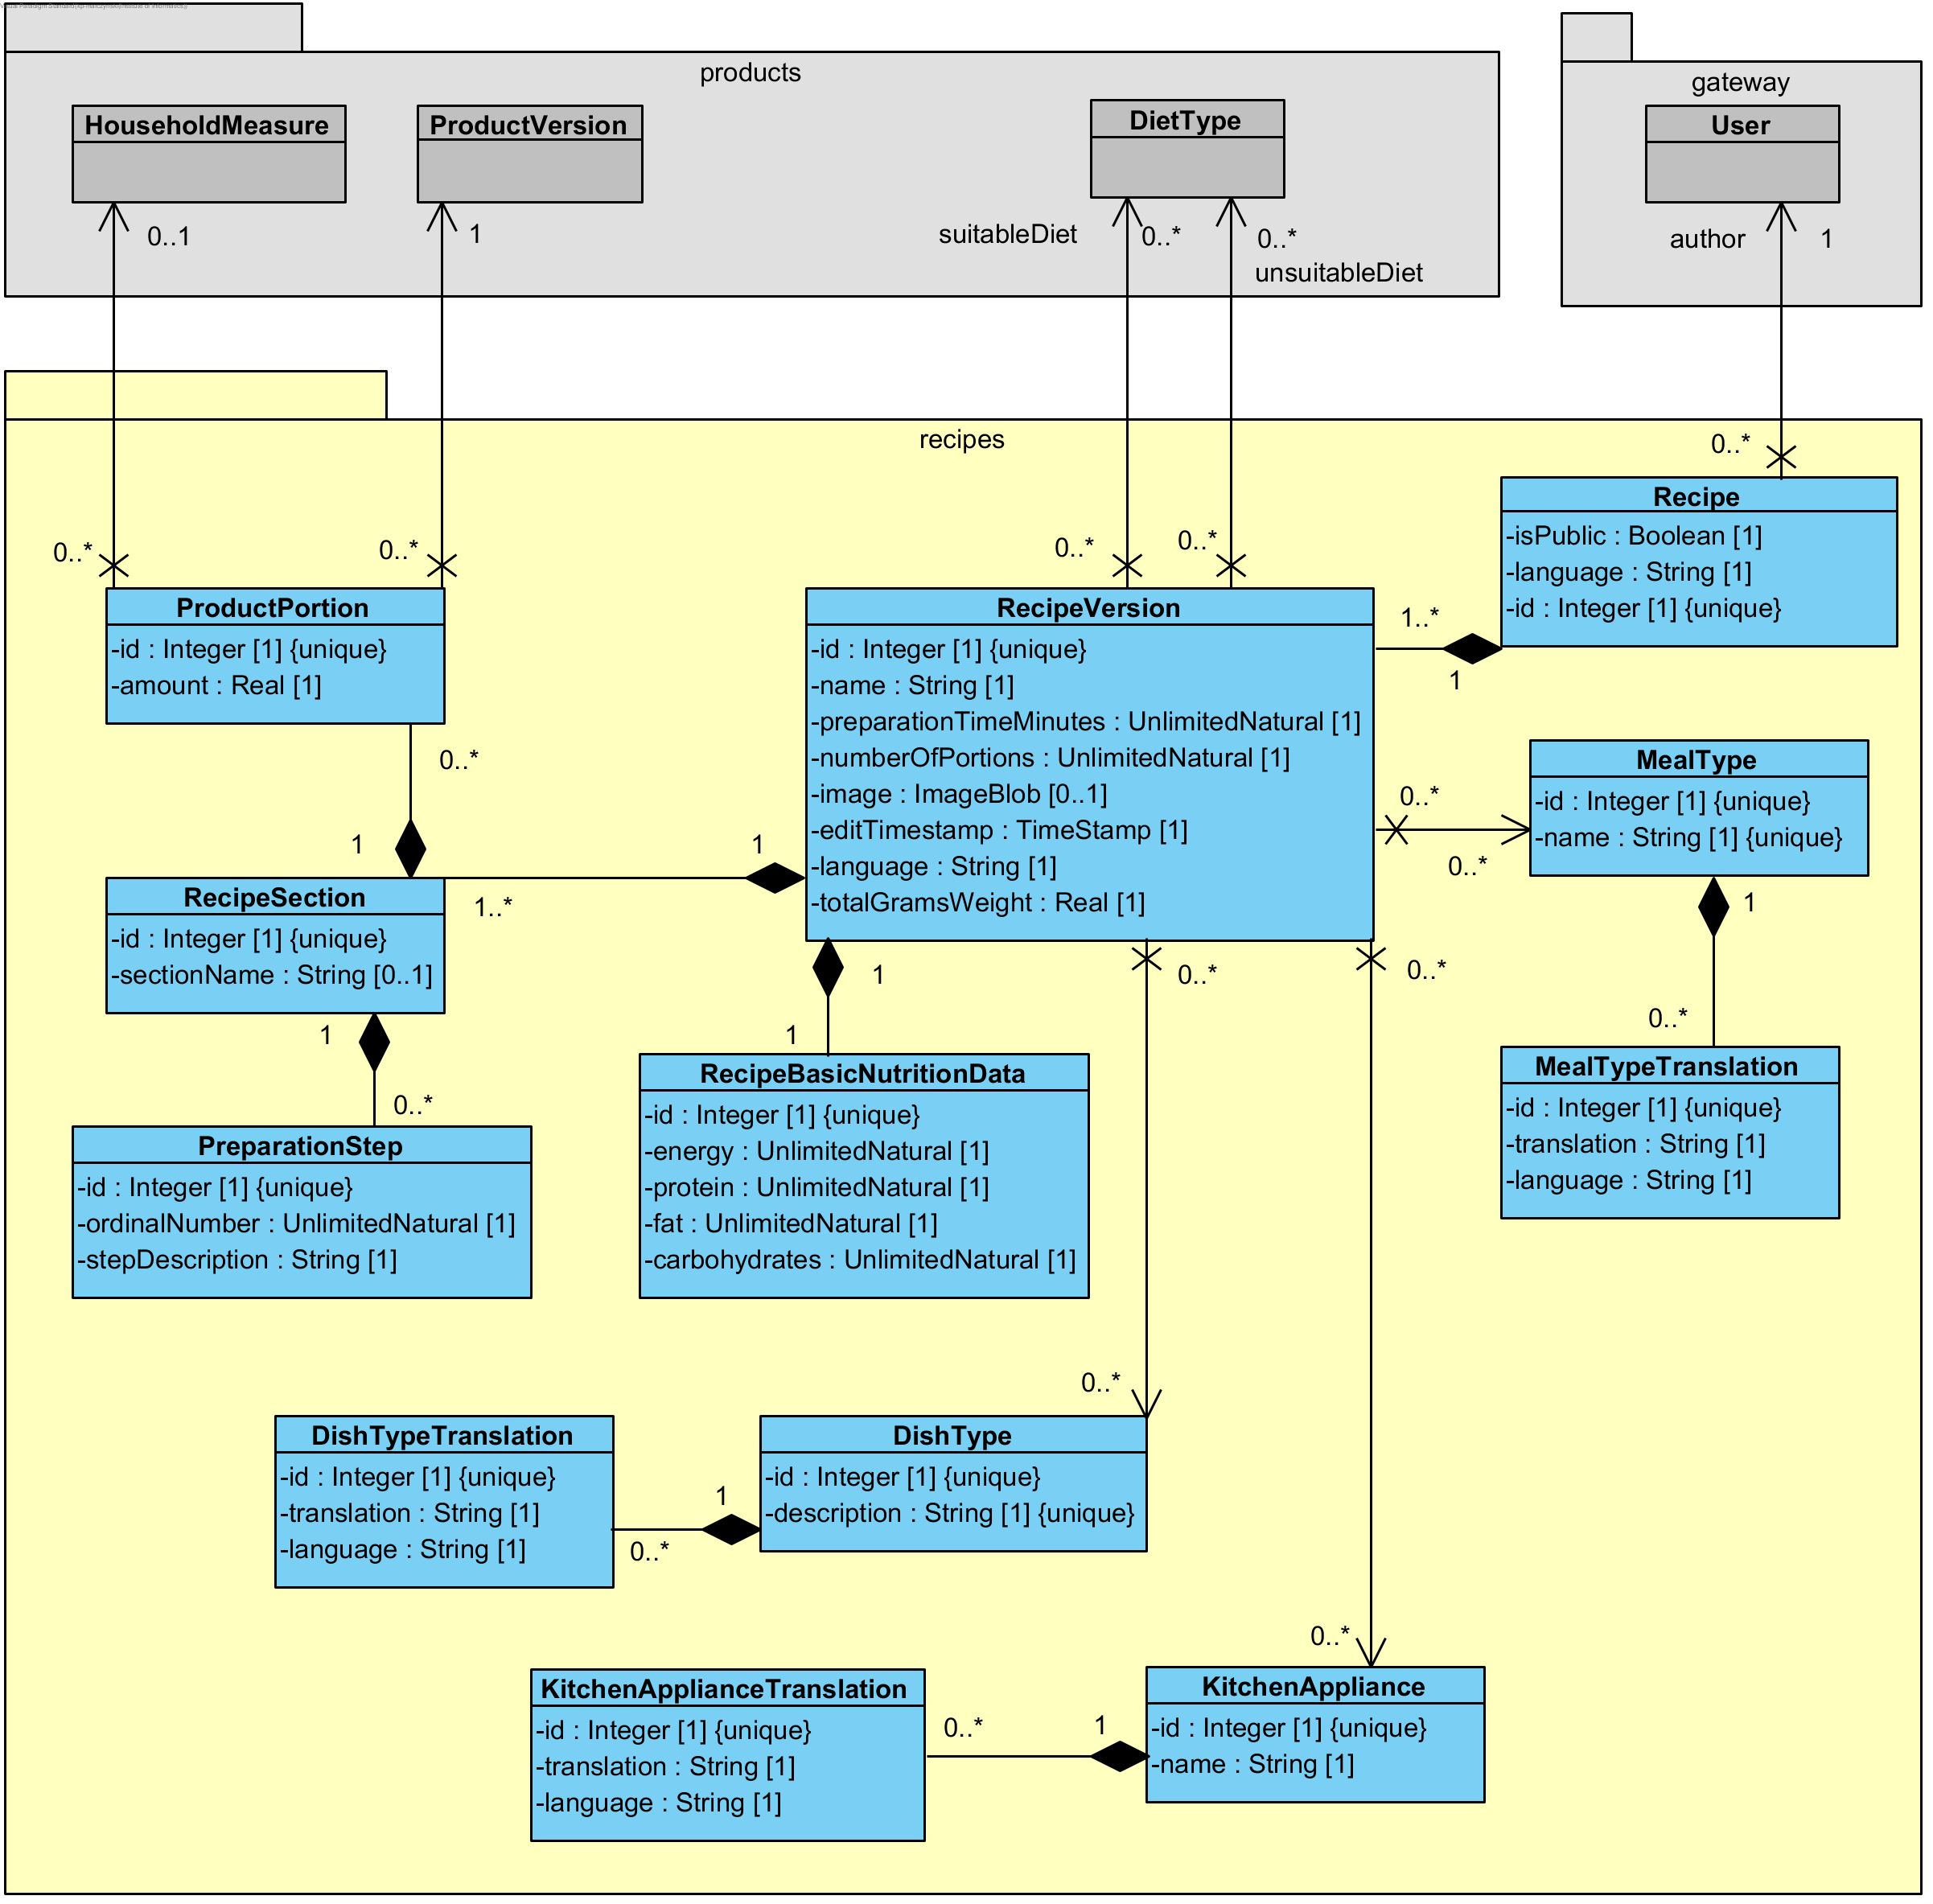
\includegraphics[scale=0.7]{../uml/class_diagrams/recipes.png}
        \caption{Przepisy - diagram klas (opr.wł).}\label{rysunek:class-diagram-recipes}
    \end{figure}
\end{minipage}

\begin{minipage}{\textwidth}
    \begin{figure}[H]
        \centering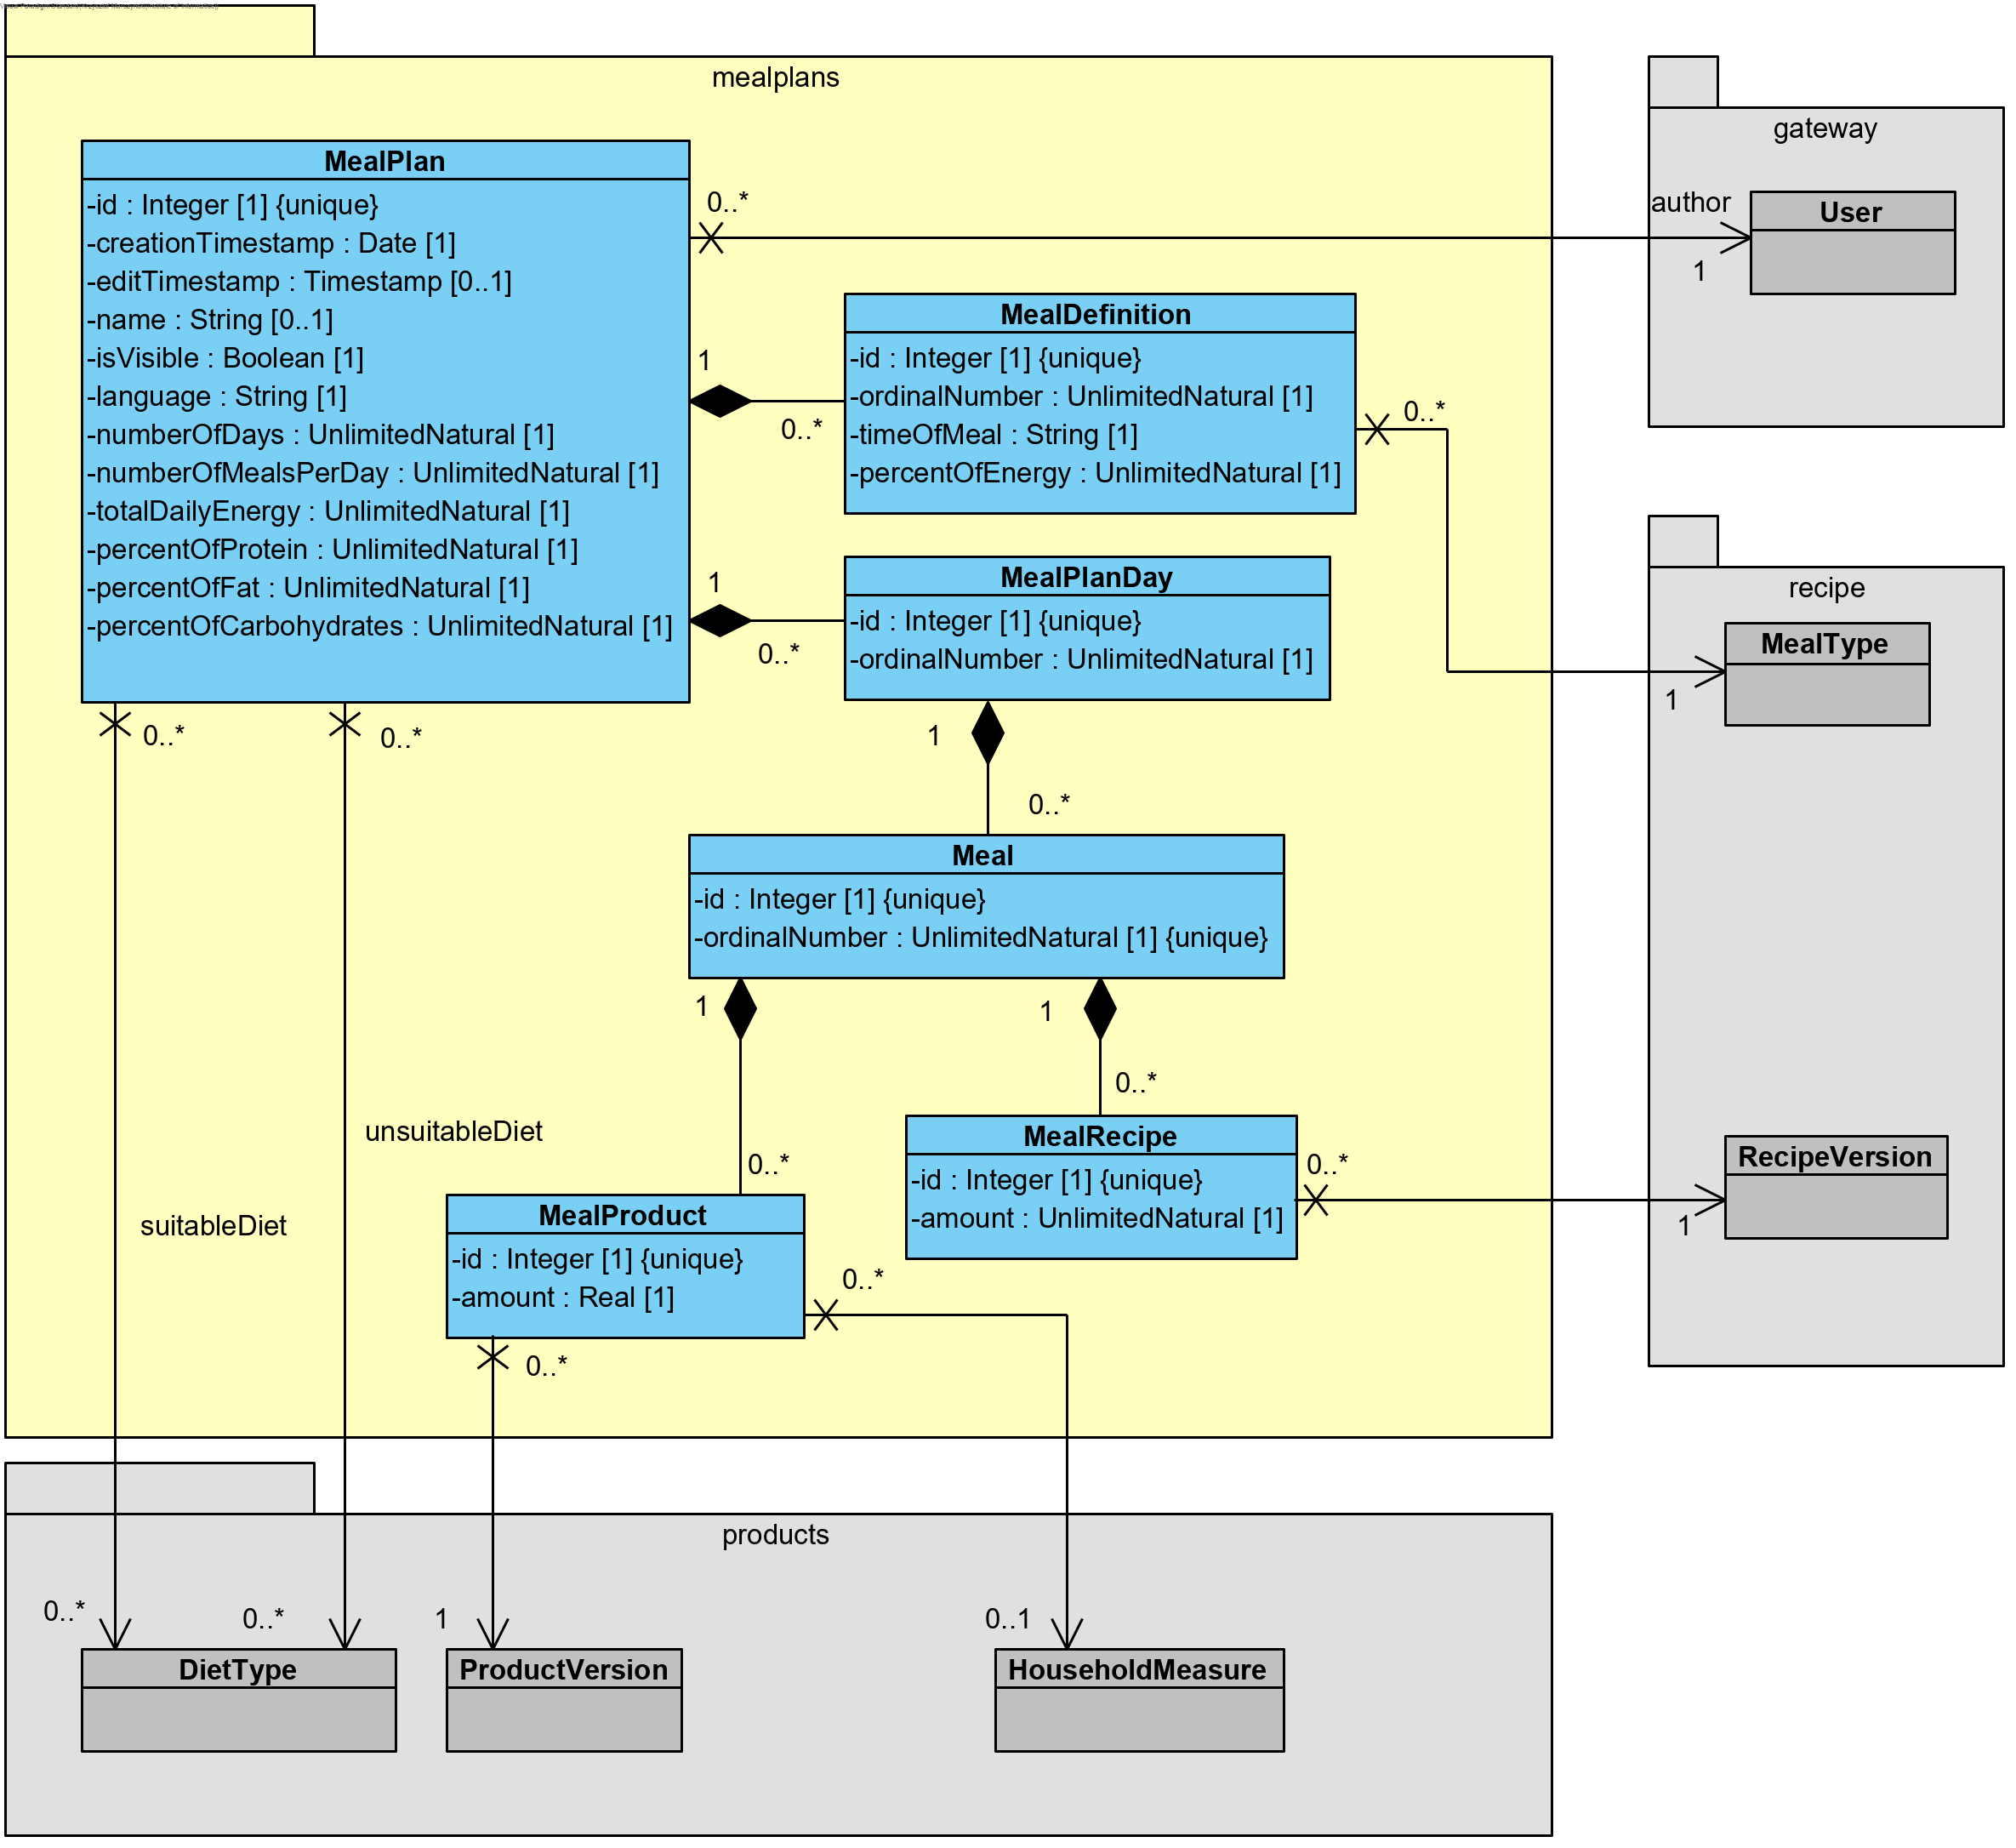
\includegraphics[scale=0.7]{../uml/class_diagrams/mealplans.png}
        \caption{Jadłospisy - diagram klas (opr.wł).}\label{rysunek:class-diagram-mealplans}
    \end{figure}
\end{minipage}

\begin{minipage}{\textwidth}
    \begin{figure}[H]
        \centering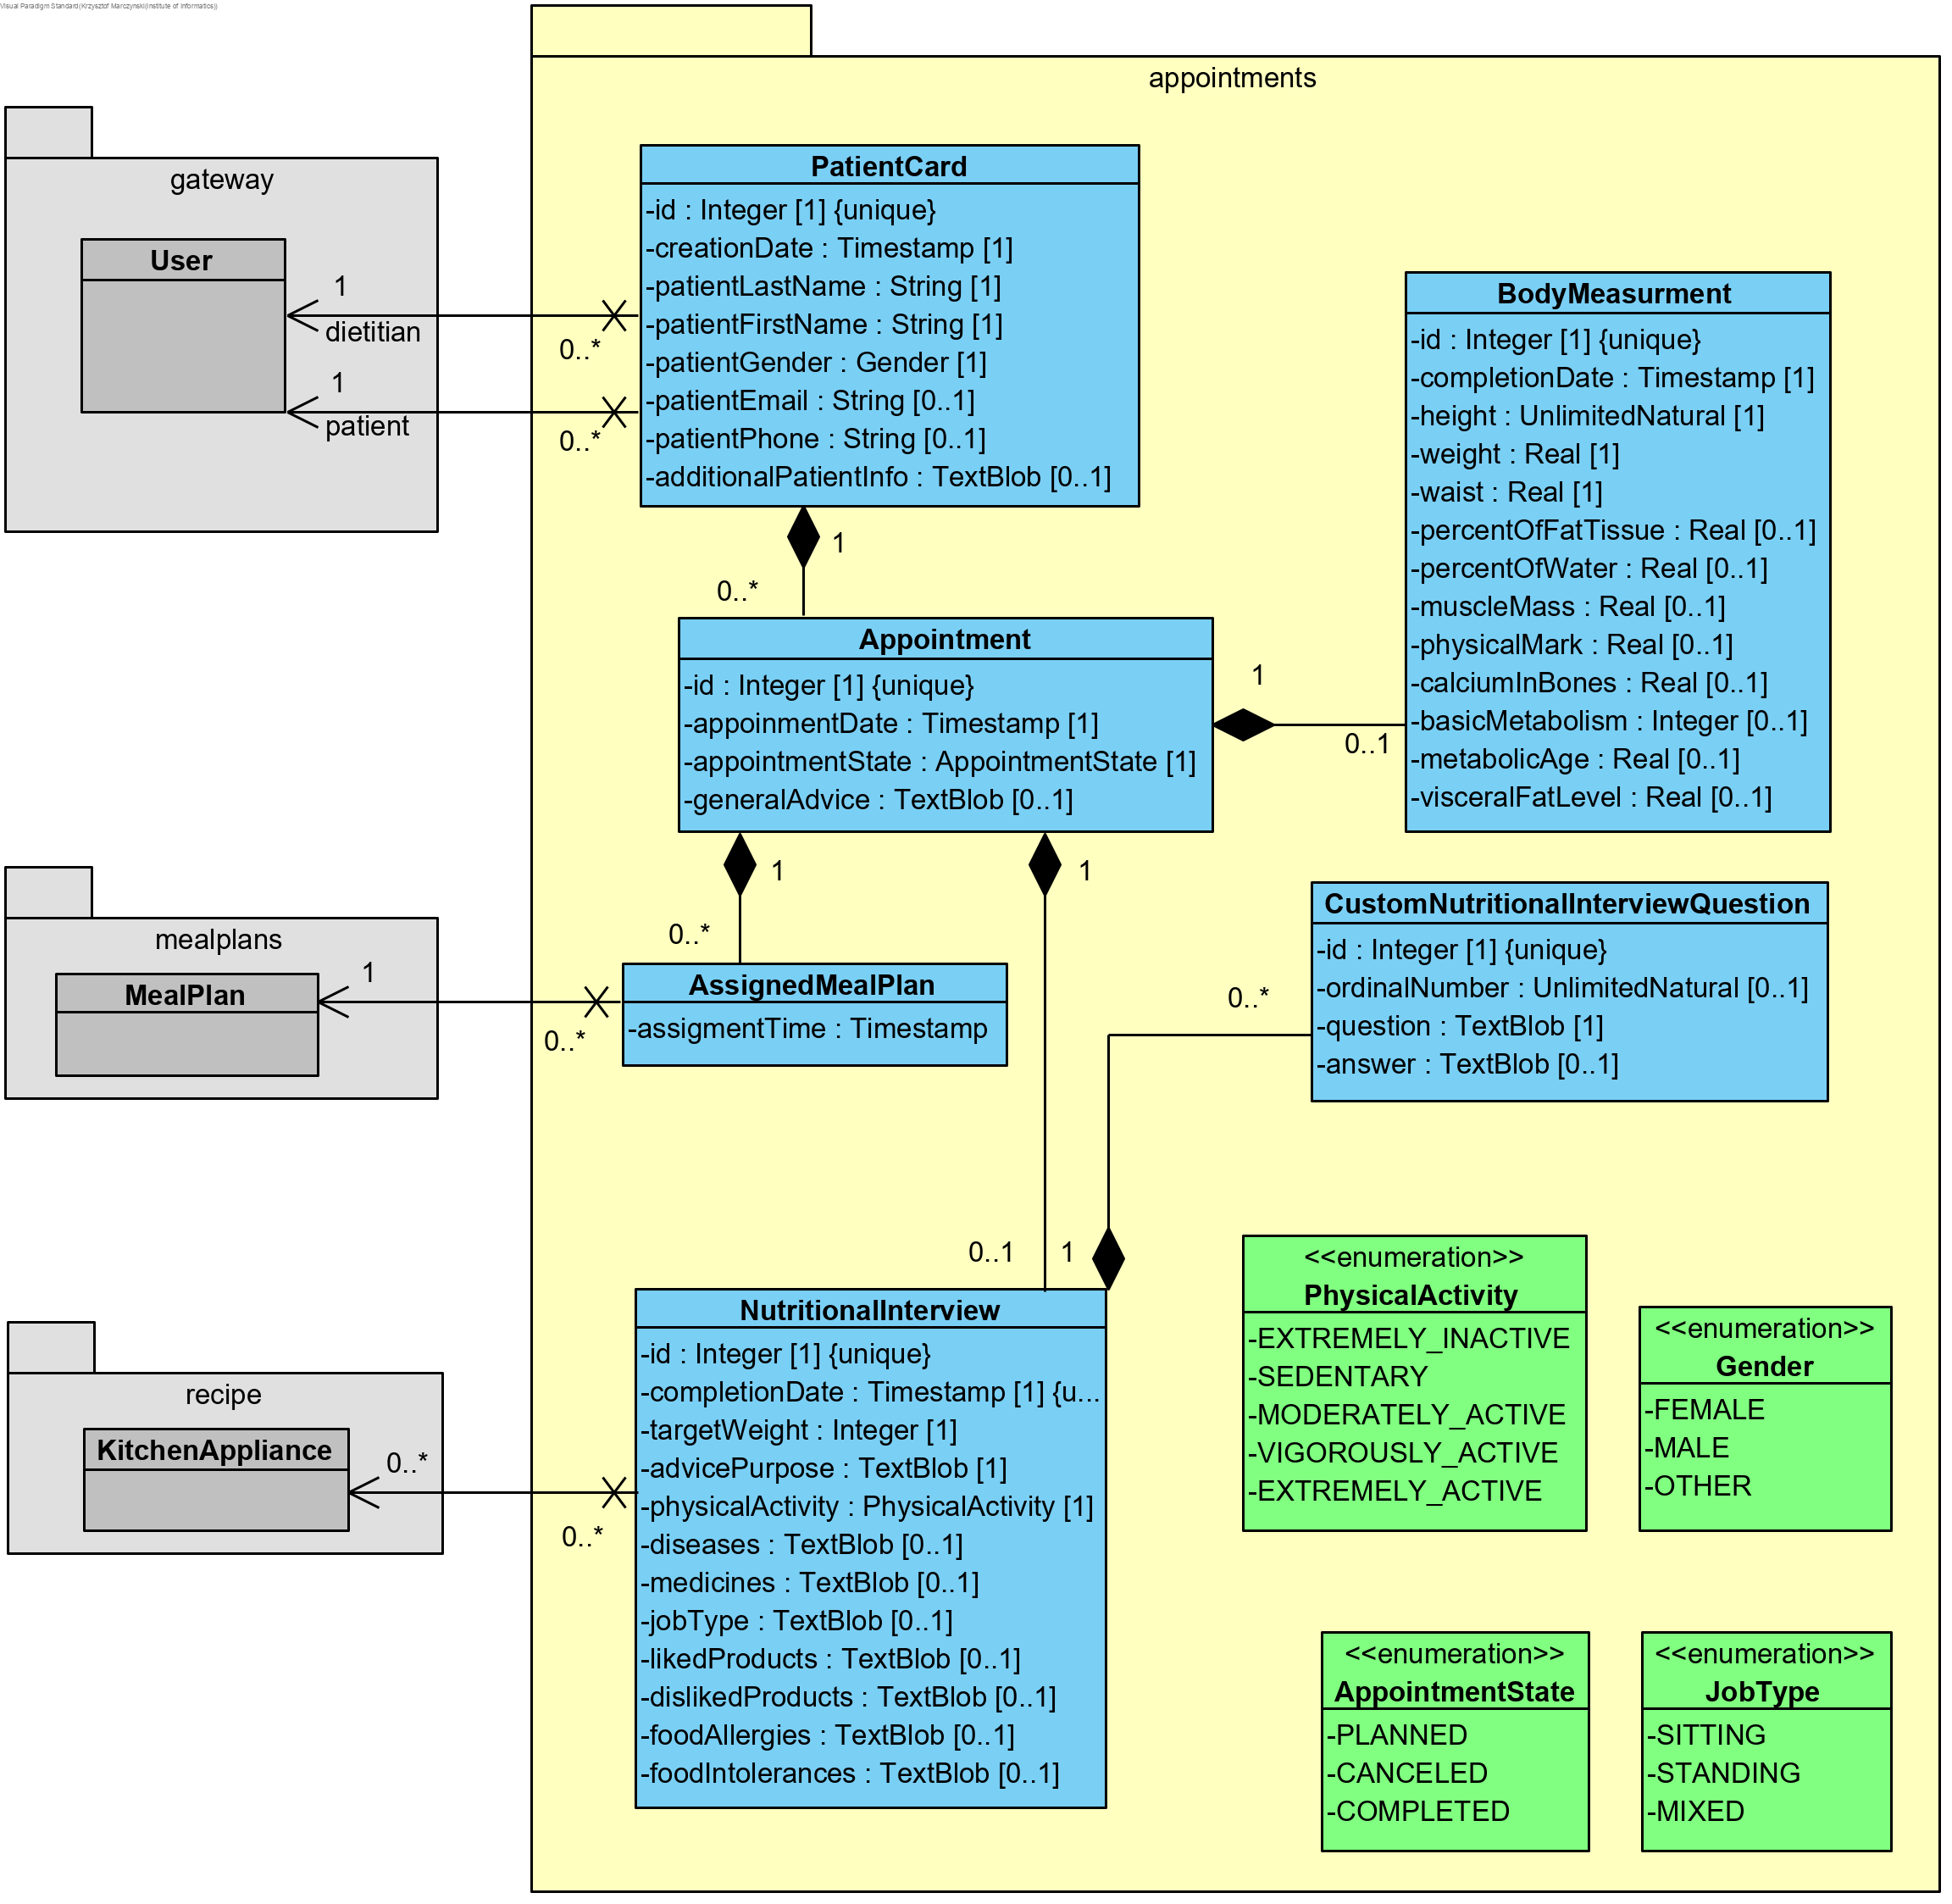
\includegraphics[scale=0.7]{../uml/class_diagrams/appointments.png}
        \caption{Wizyty - diagram klas (opr.wł).}\label{rysunek:class-diagram-appointments}
    \end{figure}
\end{minipage}



\thispagestyle{normal}

\section{Opis podstawowej architektury systemu}
\todo{Opisać, że to aplikacja webowa w architekturze mikroserwisów
Wyszczególnienie modułów;
Diagram rozmieszczenia, wzorce projektowe}

%https://martinfowler.com/eaaDev/TemporalObject.html
\thispagestyle{normal}
